\documentclass[12pt,a4paper]{article}

\usepackage[T1]{fontenc}
\usepackage{lmodern}
\usepackage[serbian]{babel}
\usepackage{authblk}
\usepackage[hidelinks]{hyperref}
\usepackage{xurl}
\usepackage{amsmath, amssymb}
\usepackage{float}
\usepackage{enumitem}
\usepackage{graphicx}
\usepackage{pdfpages}
\usepackage{booktabs}
\usepackage{multirow}
\usepackage{xcolor}
\usepackage{minted}
\usepackage{tikz}
\usetikzlibrary{positioning, fit, calc, backgrounds, shapes.geometric, babel}

\usepackage[a4paper, left=3cm, right=2.5cm, top=2.5cm, bottom=2.5cm]{geometry}

\usepackage{caption}
\captionsetup[figure]{skip=6pt}

\setminted{
	fontsize=\small,
	breaklines=true,
	autogobble=true,
	frame=single,
	bgcolor=gray!5,
	vspace=3pt,
	style=default,
}


\title{Superrezolucija video-zapisa u realnom vremenu primenom konvolucionih neuronskih mreža}
\author{Igor Jovanović, prof. dr Branimir Todorović}
\affil{\footnotesize Prirodno-matematički fakultet u Nišu, Departman za Računarske nauke}
\date{2026.}

\setlength{\emergencystretch}{3em}

\begin{document}

\begin{titlepage}
	\sffamily
	\vspace*{0.3cm}
	\noindent
	\begin{minipage}[c]{0.2\textwidth}
		\includegraphics[height=3cm]{front/logo1.png}
	\end{minipage}%
	\begin{minipage}[c]{0.6\textwidth}
		\centering\large
		\vspace{1.2cm}
		Univerzitet u Nišu\\
		Prirodno-matematički fakultet\\
		Departman za računarske nauke
	\end{minipage}%
	\begin{minipage}[c]{0.2\textwidth}
		\raggedleft
		\includegraphics[height=3cm]{front/pmf_logo2.jpg}
	\end{minipage}

	\vspace{3cm}
	\begin{center}
		{\Large\itshape Superrezolucija video-zapisa u realnom vremenu\\[2pt]
		primenom konvolucionih neuronskih mreža\par}
		\vspace{1cm}
		{\large - Master rad -\par}
	\end{center}

	\vspace{4.6cm}
	\noindent
	{\large
	\begin{minipage}[t]{0.7\textwidth}
		Mentor\\
		Prof. dr Branimir Todorović
	\end{minipage}%
	\begin{minipage}[t]{0.3\textwidth}
		Student\\
		Igor Jovanović
	\end{minipage}
	}

	\vspace{2.2cm}
	\begin{center}
		{\large Niš, 2026. godina\par}
	\end{center}
\end{titlepage}
%\setcounter{page}{2} % naslovna se broji kao strana 1, ali bez ispisanog broja

%\includepdf[pages=-]{front/kd-dipl-01.pdf}
%\includepdf[pages=-]{front/kd-dipl-02.pdf}

\newpage
\tableofcontents
\newpage


% -------------------------------------------------
\section{Uvod}
\label{sec:uvod}

U kompjuterskoj grafici, skaliranje slike (engl.\ \textit{image scaling}) označava promenu njenih prostornih dimenzija, odnosno povećanje ili smanjenje broja piksela. Kada se slika ili video-zapis prikazuje na ekranu čija je rezolucija veća od rezolucije sadržaja, sadržaj je potrebno uvećati (engl.\ \textit{upscaling}). Kvalitet tog prikaza u velikoj meri zavisi od primenjene metode uvećanja. Ovaj problem je danas sve izraženiji, ekrani visokih rezolucija postali su standard, dok je velik deo postojećeg video-sadržaja dostupan u nižoj rezoluciji (stari snimci, striming pri ograničenom protoku).

Problem povećanja rezolucije pojedinačne slike (engl.\ \textit{Single Image Super-Resolution}, SISR) može se formalno definisati na sledeći način: data je slika niske rezolucije $I^{LR} \in \mathbb{R}^{H \times W \times C}$ (engl.\ \textit{Low Resolution}), a cilj je rekonstruisati odgovarajuću sliku visoke rezolucije $I^{HR} \in \mathbb{R}^{sH \times sW \times C}$ (engl.\ \textit{High Resolution}), gde je $s$ faktor uvećanja, a $C$ broj kanala boje. Klasične interpolacijske metode procenjuju vrednosti novih piksela isključivo na osnovu susednih piksela. Brze su i jednostavne, ali ne mogu da rekonstruišu detalje kojih nema u ulaznoj slici, pa je rezultat uglavnom blago zamućen. Metode zasnovane na dubokom učenju, nasuprot tome, uče mapiranje između $I^{LR}$ i $I^{HR}$ na velikom skupu primera, pa na osnovu naučenih obrazaca mogu bolje rekonstruisati ivice i fine teksture. Savremene efikasne arhitekture pri tome postižu visok kvalitet uz relativno mali broj parametara, što otvara pitanje njihove primene i van uvećanja pojedinačnih slika.

Centralna tema ovog rada je proširenje ovog problema na uvećanje video-zapisa u realnom vremenu. Pristup je jednostavan, uvećanje pojedinačne slike primenjuje se nezavisno nad svakim frejmom. Za razliku od uvećanja pojedinačne slike, gde vreme obrade obično nije kritično, kod video-zapisa postoji strogo vremensko ograničenje: celokupna obrada jednog frejma (dekodiranje, uvećanje i priprema za prikaz) mora se završiti pre nego što treba prikazati sledeći. Za video-zapis sa $30$ frejmova u sekundi raspoloživo vreme iznosi oko $33{,}3$~ms po frejmu, a za $60$ frejmova u sekundi svega oko $16{,}7$~ms. Ako obrada traje duže, plejer mora da odbacuje frejmove, što se vidi kao trzanje (engl.\ \textit{stuttering}) i gubitak fluidnosti prikaza.

Ovo ograničenje menja kriterijum izbora modela u odnosu na klasičan SISR: nije dovoljno da model daje dobar kvalitet, već mora biti i dovoljno brz. Težište rada se zato pomera sa apsolutnog kvaliteta rekonstrukcije na odnos kvaliteta i brzine. Rad nastoji da odgovori na sledeća pitanja:
\begin{itemize}[itemsep=0pt]
	\item Kako se kvalitet i brzina standardnih arhitektura menjaju sa njihovom veličinom?
	\item Koje osobine arhitekture određuju brzinu pri zadatom kvalitetu, i da li se arhitekture efikasne po broju parametara ponašaju efikasno i po vremenu izvršavanja?
	\item Koliki se kvalitet može postići unutar vremenskog budžeta prikaza, i koliki deo tog budžeta odlazi na korake van same inferencije?
	\item U kojoj meri izvršno okruženje (PyTorch, ONNX Runtime, TensorRT, NCNN) i numerička preciznost utiču na brzinu inferencije?
\end{itemize}

Rad je organizovan na sledeći način. U poglavlju~\ref{sec:interpolacija} opisane su klasične interpolacijske metode, a u poglavlju~\ref{sec:arhitekture} arhitekture konvolucionih mreža za SISR (SRCNN, VDSR, EDSR, IMDN, RFDN i ABPN), kao i FastEDSR, sopstvena modifikacija EDSR-a prilagođena brzoj inferenciji. Poglavlja~\ref{sec:treniranje}-\ref{sec:brzina} opisuju postupak treniranja, metrike kvaliteta, način merenja brzine i izbor numeričke preciznosti. U poglavlju~\ref{sec:std_quality} data je uporedna analiza kvaliteta, veličine i brzine svih razmatranih arhitektura, a zatim se analiziraju višeskalne varijante (poglavlje~\ref{sec:viseskalni}) i modeli trenirani za JPEG-kompresovan sadržaj (poglavlje~\ref{sec:jpeg}). Poglavlje~\ref{sec:izvrsna_okruzenja} opisuje izvoz modela u format ONNX, izvršna okruženja za inferenciju i njihovo poređenje. Poglavlja~\ref{sec:plejer} i~\ref{sec:gl_sejderi} opisuju primenu modela u dva sistema za uvećanje video-zapisa u realnom vremenu. Prvi je demonstracioni video-plejer u Python-u, u osnovnoj varijanti sa dekodiranjem i prikazom na procesoru (odeljak~\ref{sec:osnovna_varijanta}) i u zero-copy varijanti sa hardverskim dekodiranjem i prikazom na grafičkoj kartici (odeljak~\ref{sec:zero_copy}). Drugi je implementacija modela u vidu GLSL šejdera za postojeći plejer \texttt{mpv}, bez zavisnosti od izvršnog okruženja za neuronske mreže. Poglavlje~\ref{sec:zakljucak} iznosi zaključke rada. Kompletan izvorni kod projekta, uključujući skripte za treniranje i evaluaciju modela, implementacije video-plejera i generator šejdera, dostupan je u repozitorijumu na adresi \url{https://github.com/ig0r2/super-resolution-cnn}.
% ----------------------------------------------

%-----------------------------------------------------
\section{Interpolacijske metode}
\label{sec:interpolacija}

Klasične metode povećanja rezolucije zasnivaju se na interpolaciji postojećih vrednosti piksela. Razmatrane metode mogu se implementirati korišćenjem različitih interpolacionih jezgara (engl.\ \textit{kernels}), tako da se dvodimenzionalna interpolacija može zapisati u obliku \cite{meijering2002}:
\begin{equation}
	\hat{I}(x,y) = \sum_{i}\sum_{j} I(x_i, y_j)\, h(x - x_i)\, h(y - y_j),
\end{equation}
gde je $(x,y)$ položaj izlaznog piksela preslikan u koordinatni sistem ulazne slike, $(x_i,y_j)$ položaji piksela ulazne slike, a $h$ jednodimenzionalno interpolaciono jezgro. Jezgro se primenjuje posebno po svakoj osi. Metode se razlikuju po obliku i veličini jezgra, što utiče na računsku složenost i kvalitet rekonstruisane slike.

\subsection{Interpolacija najbližeg suseda}

Kod interpolacije najbližeg suseda (engl.\ \textit{Nearest Neighbor}) svaki novi piksel dobija vrednost prostorno najbližeg piksela ulazne slike. Ova operacija odgovara pravougaonom jezgru:
\begin{equation}
	h(x) =
	\begin{cases}
		1, & |x| < 0{,}5, \\
		0, & \text{inače.}
	\end{cases}
\end{equation}

Ova metoda ima najmanju računsku složenost, ali pri uvećanju slike dovodi do izraženih blokova iste boje, jer se jedna vrednost ulaznog piksela preslikava na više izlaznih piksela.

\subsection{Bilinearna interpolacija}

Kod bilinearne (engl.\ \textit{Bilinear}) interpolacije vrednost novog piksela određuje se težinskom kombinacijom četiri najbliža piksela. Odgovarajuće jednodimenzionalno jezgro je trougaonog oblika:

\begin{equation}
	h(x) =
	\begin{cases}
		1 - |x|, & |x| < 1, \\
		0, & \text{inače.}
	\end{cases}
\end{equation}

Rezultat je vizuelno glađi nego kod interpolacije najbližeg suseda, ali interpolacija istovremeno prigušuje deo visokofrekventnih komponenti slike, što se primećuje kao zamućenje.

\subsection{Bikubna interpolacija}

Bikubna (engl.\ \textit{Bicubic}) interpolacija koristi $4 \times 4$ okolinu, odnosno 16 susednih piksela. Kubno interpolaciono jezgro ima oblik \cite{keys1981}:

\begin{equation}
	h(x) =
	\begin{cases}
		1{,}5|x|^3 - 2{,}5|x|^2 + 1, & |x| < 1, \\
		-0{,}5|x|^3 + 2{,}5|x|^2 - 4|x| + 2, & 1 \le |x| < 2, \\
		0, & \text{inače.}
	\end{cases}
\end{equation}

Bikubna interpolacija predstavlja jednu od najčešće korišćenih metoda skaliranja slike. U literaturi o superrezoluciji naročito je česta upotreba bikubnog smanjivanja rezolucije za generisanje sintetičkih LR slika iz odgovarajućih HR slika, kao i referentna metoda pri evaluaciji modela.

\subsection{Lanczosova interpolacija}

Lanczosova interpolacija koristi prozorsko sinc jezgro \cite{duchon1979}:

\begin{equation}
	h(x) =
	\begin{cases}
		1, & x = 0, \\[4pt]
		\dfrac{a \sin(\pi x)\sin(\frac{\pi x}{a})}
		{\pi^2x^2}, & 0 < |x| < a, \\[6pt]
		0, & |x| \ge a,
	\end{cases}
\end{equation}

gde parametar $a$, najčešće $a=2$ ili $a=3$, određuje veličinu jezgra. Lanczosova interpolacija može bolje očuvati oštre prelaze i visokofrekventne komponente od prethodno navedenih interpolacionih metoda, ali može doći do pojave artefakata prstenovanja (engl.\ \textit{ringing}).

Zajedničko ograničenje interpolacionih metoda jeste to što izlaz određuju isključivo na osnovu lokalnih vrednosti postojećih piksela. One ne koriste prethodno naučeno znanje o strukturi prirodnih slika i zato ne mogu pouzdano rekonstruisati nedostajuće fine teksture.

%-----------------------------------------------------
\section{Arhitekture konvolucionih mreža za SISR}
\label{sec:arhitekture}

Pristupi zasnovani na dubokom učenju najčešće formulišu problem SISR kao regresioni zadatak. Cilj je naučiti parametre mreže tako da njen izlaz bude što sličniji odgovarajućoj referentnoj HR slici. Ako sa $I^{LR}$ označimo ulaz mreže, parametri mreže $\theta$ mogu se odrediti minimizacijom funkcije gubitka:
\begin{equation}
	\hat{\theta}
	=
	\arg\min_{\theta}
	L\bigl(F_{\theta}(I^{LR}), I^{HR}\bigr),
\end{equation}
gde $F_{\theta}$ predstavlja preslikavanje koje realizuje neuronska mreža, dok $L$ označava funkciju gubitka.

Različite arhitekture razlikuju se po organizaciji slojeva, dubini i širini mreže, mestu na kome se vrši uvećanje prostorne rezolucije, upotrebi rezidualnih veza i mehanizama pažnje, kao i po strategiji treniranja. Takođe, u zavisnosti od arhitekture, ulaz mreže može biti originalna LR slika ili LR slika koja je prethodno interpolirana na ciljnu rezoluciju.

%---------------------------SRCNN BEGIN
\subsection{SRCNN}

SRCNN \cite{SRCNN} predstavlja jednu od prvih uspešnih primena konvolucionih neuronskih mreža za direktno učenje mapiranja između slika niske i visoke rezolucije. Značajan doprinos rada predstavlja dokaz da se postupci zasnovani na retkom kodiranju (engl.\ \textit{sparse coding}) \cite{yang2010} mogu interpretirati kroz niz konvolucionih operacija.

Kod SRCNN-a ulaz u mrežu nije originalna LR slika. Ona se najpre bikubnom interpolacijom uvećava na željene prostorne dimenzije, obeležićemo je sa $I^{LR}_{bic}$. Mreža stoga sama ne povećava broj piksela, već transformiše prethodno interpoliranu sliku:
\begin{equation}
	I^{SR} = F_{\theta}(I^{LR}_{bic}).
\end{equation}

Osnovna SRCNN arhitektura sastoji se od tri konvoluciona sloja, od kojih svaki ima konceptualno posebnu ulogu.

\textbf{1. Ekstrakcija i reprezentacija isečaka}
(engl.\ \textit{patch extraction and representation}):
prvi konvolucioni sloj primenjuje $n_1$ filtera sa konvolucionim jezgrom (engl. \textit{kernel}) veličine $f_1 \times f_1$ nad ulaznim kanalima, nakon čega se primenjuje ReLU aktivaciona funkcija:
\begin{equation}
	F_1(Y) = \max(0,\,W_1 * Y + B_1).
\end{equation}

Ovaj korak konceptualno odgovara izdvajanju isečaka i njihovom predstavljanju pomoću rečnika u pristupima zasnovanim na retkom kodiranju.

\textbf{2. Nelinearno mapiranje}
(engl.\ \textit{non-linear mapping}):
drugi konvolucioni sloj koristi $n_2$ filtera nad $n_1$ ulaznih mapa obeležja (engl. \textit{feature maps}) sa konvolucionim jezgrom veličine $f_2 \times f_2$, čime se transformiše reprezentacija dobijena prethodnim slojem:
\begin{equation}
	F_2(Y) = \max(0,\,W_2 * F_1(Y) + B_2).
\end{equation}

U osnovnoj konfiguraciji koristi se konvoluciono jezgro veličine $1 \times 1$. Takva konvolucija kombinuje informacije između kanala na istoj prostornoj poziciji, bez korišćenja piksela na susednim pozicijama.

\textbf{3. Rekonstrukcija}:
poslednji konvolucioni sloj kombinuje dobijena obeležja iz susednih pozicija i formira izlaznu sliku, bez korišćenja aktivacione funkcije:
\begin{equation}
	F(Y) = W_3 * F_2(Y) + B_3.
\end{equation}

\begin{figure}[H]
	\centering
	\begin{tikzpicture}[
	font=\sffamily\small,
	node distance=5mm,
	>=stealth,
	blk/.style={draw, rounded corners=3pt, align=center, minimum height=11mm, inner sep=1mm},
	io/.style={blk, fill=gray!15, draw=gray!60, minimum width=9mm},
	interp/.style={blk, fill=yellow!45!orange!35, draw=orange!50, minimum width=24mm},
	conv/.style={blk, fill=cyan!20, draw=cyan!50, minimum width=14mm},
	relu/.style={blk, fill=violet!12, draw=violet!40, minimum width=12mm},
	lbl/.style={align=center, below=1.5mm}
	]
	\node[io] (lr) {LR};
	\node[interp, right=of lr] (bic) {Bikubna\\interpolacija};
	\node[conv, right=of bic] (c1) {Conv\\9\,\texttimes\,9};
	\node[relu, right=0mm of c1] (r1) {ReLU};
	\node[conv, right=of r1] (c2) {Conv\\1\,\texttimes\,1};
	\node[relu, right=0mm of c2] (r2) {ReLU};
	\node[conv, right=of r2] (c3) {Conv\\5\,\texttimes\,5};
	\node[io, right=of c3] (sr) {SR};

	\draw[->] (lr) -- (bic);
	\draw[->] (bic) -- (c1);
	\draw[->] (r1) -- (c2);
	\draw[->] (r2) -- (c3);
	\draw[->] (c3) -- (sr);

	\node[lbl] at ($(c1.south west)!0.5!(r1.south east)$) {Ekstrakcija\\delova};
	\node[lbl] at ($(c2.south west)!0.5!(r2.south east)$) {Nelinearno\\mapiranje};
	\node[lbl] at (c3.south) {Rekonstrukcija};
\end{tikzpicture}

	\caption{Arhitektura SRCNN mreže.}
	\label{fig:srcnn}
\end{figure}

U standardnom modelu koji obrađuje samo luminansni (Y) kanal ulaz i izlaz imaju samo jedan kanal, dok proširena verzija koja istovremeno obrađuje tri kanala ima tri ulazna i tri izlazna kanala.
Standardna konfiguracija koristi $f_1=9$, $f_2=1$, $f_3=5$, $n_1=64$ i $n_2=32$. Promenom broja filtera i veličine njihovih konvolucionih jezgara moguće je menjati odnos između kvaliteta rekonstrukcije i računske složenosti.

\subsubsection{Treniranje}

Osnovni SRCNN eksperimenti koriste trening skup \textit{T91} \cite{yang2010}, koji sadrži 91 sliku. Iz njih se izdvajaju približno 24\,800 preklapajućih isečaka veličine $33 \times 33$ piksela, sa korakom (engl.\ \textit{stride}) od 14 piksela. U osnovnim eksperimentima sa ovim skupom ne koristi se geometrijsko proširivanje skupa podataka (engl.\ \textit{data augmentation}), poput rotiranja i refleksije slika. Većina eksperimenata sprovodi se nad kanalom luminanse, slike se konvertuju u YCbCr prostor boja, a model obrađuje samo Y kanal. U proširenoj verziji rada autori eksperimentišu i sa mrežom koja istovremeno obrađuje sva tri kanala, uključujući direktno treniranje u RGB prostoru. Kao funkcija gubitka koristi se srednja kvadratna greška (engl.\ \textit{Mean Squared Error}, MSE), odnosno $\ell_2$ gubitak:
\begin{equation}
	L(\theta)
	=
	\frac{1}{n}
	\sum_{i=1}^{n}
	\left\|
	I^{SR}_i-I^{HR}_i
	\right\|_2^2.
\end{equation}

Optimizacija se sprovodi stohastičkim gradijentnim spustom (engl.\ \textit{Stochastic Gradient Descent}, SGD). U osnovnoj konfiguraciji autori koriste stopu učenja $10^{-4}$ za prva dva sloja i manju stopu $10^{-5}$ za poslednji sloj. Model se trenira kroz $8\times10^8$ propagacija greške unazad.

%---------------------------SRCNN END

\subsection{VDSR - Very Deep Convolutional Networks}

VDSR \cite{VDSR} značajno povećava dubinu konvolucionih modela za SISR i zasnovan je na principima VGG mreže \cite{VGG}. Za razliku od troslojnog SRCNN-a, VDSR koristi 20 konvolucionih slojeva. Ključne ideje koje omogućavaju uspešno treniranje ovako duboke mreže jesu rezidualno učenje, visoka početna stopa učenja i adaptivno odsecanje gradijenata.

Prvi konvolucioni sloj generiše 64 mape obeležja pomoću konvolucionih jezgara veličine $3\times3$. Nakon njega sledi 18 konvolucionih slojeva sa po 64 izlazna kanala i jezgrima veličine $3\times3$, dok poslednji, dvadeseti sloj generiše rezidualnu sliku. ReLU aktivaciona funkcija primenjuje se nakon prvih 19 konvolucionih slojeva, dok poslednji sloj nema aktivacionu funkciju. Zbog sukcesivne primene 20 konvolucija sa jezgrima veličine $3\times3$, receptivno polje izlaznog piksela iznosi $41\times41$ piksela. Na taj način mreža može da koristi znatno širi prostorni kontekst nego SRCNN bez potrebe za korišćenjem velikih konvolucionih jezgara.

\begin{figure}[H]
	\centering
	\begin{tikzpicture}[
	font=\sffamily\small,
	node distance=5mm,
	>=stealth,
	blk/.style={draw, rounded corners=3pt, align=center, minimum height=11mm, inner sep=1mm},
	io/.style={blk, fill=gray!15, draw=gray!60, minimum width=9mm},
	interp/.style={blk, fill=yellow!45!orange!35, draw=orange!70, minimum width=24mm},
	conv/.style={blk, fill=cyan!20, draw=cyan!50!black, minimum width=14mm},
	relu/.style={blk, fill=violet!12, draw=violet!40, minimum width=12mm},
	op/.style={circle, draw=gray!50, fill=gray!20, minimum size=8mm, inner sep=0pt}
	]
	\node[io] (lr) {LR};
	\node[interp, right=of lr] (bic) {Bikubna\\interpolacija};
	\node[conv, right=7mm of bic] (c1) {Conv\\3\,\texttimes\,3};
	\node[relu, right=0mm of c1] (r1) {ReLU};
	\node[right=of r1] (dots) {$\cdots$};
	\node[conv, right=of dots] (c2) {Conv\\3\,\texttimes\,3};
	\node[op, right=of c2] (add) {$+$};
	\node[io, right=of add] (sr) {SR};

	\draw[->] (lr) -- (bic);
	\draw[->] (bic) -- (c1);
	\draw[->] (r1) -- (dots);
	\draw[->] (dots) -- (c2);
	\draw[->] (c2) -- (add);
	\draw[->] (add) -- (sr);
	\coordinate (split) at ($(bic.east)!0.5!(c1.west)$);
	\draw[->] (split) -- ++(0,-9mm) -| (add.south);
\end{tikzpicture}

	\caption{Arhitektura VDSR mreže.}
	\label{fig:vdsr}
\end{figure}

Kao i SRCNN, VDSR na ulazu prima LR sliku koja je prethodno uvećana bikubnom interpolacijom na ciljnu rezoluciju. Međutim, umesto direktnog predviđanja HR slike, mreža uči rezidual:
\begin{equation}
	r = I^{HR} - I^{LR}_{bic}
\end{equation}

\begin{equation}
	\hat{\theta}
	=
	\arg\min_{\theta}
	L\bigl(F_{\theta}(I^{LR}_{bic}), r\bigr).
\end{equation}
Izlazna SR slika dobija se sabiranjem predviđenog reziduala i interpolirane ulazne slike:
\begin{equation}
	\label{eq:VDSR}
	I^{SR}
	=
	I^{LR}_{bic}
	+
	F_{\theta}(I^{LR}_{bic}).
\end{equation}

Intuicija ovog pristupa jeste da bikubno interpolirana slika već sadrži veliki deo niskofrekventne strukture originalne slike. Mreža zato ne mora da uči modelovanje cele slike, već samo kako da poboljša već interpoliranu sliku. Autori pokazuju da ovakvo rezidualno učenje znatno ubrzava konvergenciju.

\subsubsection{Treniranje}

VDSR takođe koristi srednju kvadratnu grešku kao funkciju gubitka. Optimizacija se sprovodi stohastičkim gradijentnim spustom sa momentom $0{,}9$ i regularizacijom težina (engl.\ \textit{weight decay}) od $10^{-4}$. Posebno važan deo postupka treniranja predstavlja veoma visoka početna stopa učenja. Ona je postavljena na $0{,}1$, a smanjuje se deset puta svakih 20 epoha, tokom ukupno 80 epoha treniranja. Visoka stopa učenja ubrzava konvergenciju, ali istovremeno povećava rizik od pojave veoma velikih gradijenata, zbog čega VDSR uvodi adaptivno odsecanje gradijenata (engl.\ \textit{adjustable gradient clipping}). Gradijenti se ograničavaju na interval $
\left[
-\frac{\delta}{\gamma},
\frac{\delta}{\gamma}
\right] ,$
gde je $\gamma$ trenutna stopa učenja, dok je $\delta$ parametar odsecanja. Na ovaj način se efektivni prag odsecanja prilagođava promeni stope učenja. Kombinacija ove tehnike i rezidualnog učenja omogućava stabilno korišćenje visoke početne stope učenja.

Važan doprinos VDSR-a predstavlja i višeskalno treniranje (engl.\ \textit{multi-scale training}). Umesto zasebnog modela za svaki faktor uvećanja ($\times2$, $\times3$ i $\times4$), isti model može se trenirati primerima iz više skala. Pošto je ulaz mreže u svim slučajevima već interpoliran na ciljnu rezoluciju, arhitekturu nije potrebno menjati u zavisnosti od faktora uvećanja. Autori pokazuju da ovakav višeskalni model postiže rezultate uporedive sa odgovarajućim modelima treniranim za pojedinačne faktore uvećanja.

%---------------------------------------------------------------
\subsection{EDSR - Enhanced Deep Super-Resolution Network}

EDSR \cite{EDSR} je razvijen polazeći od SRResNet \cite{SRGAN2017} arhitekture, pri čemu autori pojednostavljuju rezidualne blokove i zatim značajno povećavaju širinu i dubinu mreže.

Važna razlika u odnosu na SRCNN i VDSR jeste mesto na kome se vrši uvećanje rezolucije. EDSR ne prima unapred bikubno uvećanu sliku, već direktno obrađuje LR sliku u njenoj originalnoj prostornoj rezoluciji. Veći deo izračunavanja zato se obavlja u LR prostoru, a uvećanje se vrši tek pri kraju mreže.

Mreža počinje konvolucionim slojem koji izdvaja početna obeležja iz LR slike. Sledi telo mreže, koje se sastoji od niza rezidualnih blokova \cite{ResNet} i dodatne konvolucije. Izlaz tela se sabira sa početnim obeležjima preko duge rezidualne veze. Prostorna rezolucija se uvećava tek nakon toga, pomoću sub-pikselne konvolucije (engl.\ \textit{sub-pixel convolution}) \cite{ESPCN}. Na kraju završni konvolucioni sloj od uvećanih obeležja formira SR sliku.

\begin{figure}[H]
	\centering
	\resizebox{\textwidth}{!}{\begin{tikzpicture}[
	font=\sffamily\small,
	node distance=5mm,
	>=stealth,
	blk/.style={draw, rounded corners=3pt, align=center, minimum height=11mm, inner sep=1mm},
	io/.style={blk, fill=gray!15, draw=gray!60, minimum width=9mm},
	conv/.style={blk, fill=cyan!40, draw=cyan!70, minimum width=14mm},
	relu/.style={blk, fill=violet!12, draw=violet!40, minimum width=12mm},
	res/.style={blk, fill=green!50!black!15, draw=green!50!black!60, minimum width=20mm},
	ps/.style={blk, fill=yellow!45!orange!35, draw=orange!50, minimum width=24mm},
	op/.style={circle, draw=gray!50, fill=gray!20, minimum size=8mm, inner sep=0pt}
	]
	% --- glavni tok ---
	\node[io] (lr) {LR};
	\node[conv, right=of lr] (m1) {Conv\\3\,\texttimes\,3};
	\node[res, right=7mm of m1] (rb1) {ResBlock};
	\node[right=3mm of rb1] (dots) {$\cdots$};
	\node[res, right=3mm of dots] (rb2) {ResBlock};
	\node[conv, right=of rb2] (m2) {Conv\\3\,\texttimes\,3};
	\node[op, right=of m2] (add) {$+$};
	\node[ps, right=of add] (ps) {Sub-pixel\\Conv};
	\node[conv, right=of ps] (m3) {Conv\\3\,\texttimes\,3};
	\node[io, right=of m3] (sr) {SR};

	\draw[->] (lr) -- (m1);
	\draw[->] (m1) -- (rb1);
	\draw[->] (rb1) -- (dots);
	\draw[->] (dots) -- (rb2);
	\draw[->] (rb2) -- (m2);
	\draw[->] (m2) -- (add);
	\draw[->] (add) -- (ps);
	\draw[->] (ps) -- (m3);
	\draw[->] (m3) -- (sr);
	\coordinate (split) at ($(m1.east)!0.5!(rb1.west)$);
	\draw[->] (split) -- ++(0,-9mm) -| (add.south);

	% --- detalj rezidualnog bloka ---
	\coordinate (bin) at ($(lr.west)+(0,29mm)$);
	\node[conv, right=7mm of bin] (bc1) {Conv\\3\,\texttimes\,3};
	\node[relu, right=0mm of bc1] (br) {ReLU};
	\node[conv, right=0mm of br] (bc2) {Conv\\3\,\texttimes\,3};
	\node[op, right=8mm of bc2] (mul) {$*$};
	\node[op, above=4mm of mul] (alpha) {$\alpha$};
	\node[op, right=6mm of mul] (badd) {$+$};
	\coordinate[right=7mm of badd] (bout);

	\draw[->] (bin) -- (bc1);
	\draw[->] (bc2) -- (mul);
	\draw[->] (alpha) -- (mul);
	\draw[->] (mul) -- (badd);
	\draw[->] (badd) -- (bout);
	\coordinate (bsplit) at ($(bin)!0.5!(bc1.west)$);
	\coordinate (bbot) at ($(bsplit)+(0,-9mm)$);
	\draw[->] (bsplit) -- (bbot) -| (badd.south);

	\node[anchor=south west] (title) at ($(bin)+(1mm,11mm)$) {ResBlock};
	\begin{scope}[on background layer]
		\node[draw=green!50!black!40, fill=green!50!black!4, rounded corners=6pt, inner sep=3mm,
			fit=(bin)(title)(alpha)(bout)(bbot)] {};
	\end{scope}
\end{tikzpicture}
}
	\caption{Arhitektura EDSR mreže.}
	\label{fig:edsr}
\end{figure}

Sub-pikselna konvolucija sastoji se od konvolucije praćene operacijom preraspoređivanja piksela (engl.\ \textit{Pixel Shuffle}). Operacija PixelShuffle nema parametre i ne vrši nikakvo izračunavanje, već samo preraspoređuje elemente tenzora. Za faktor uvećanja $s$, prethodna konvolucija daje tenzor sa $C s^2$ kanala dimenzija $H\times W$, a PixelShuffle ga preslikava u tenzor sa $C$ kanala dimenzija $sH\times sW$:
\begin{equation}
	\mathbf{Y}_{c,\, y,\, x}
	=
	\mathbf{X}_{c s^2 + s\,(y \bmod s) + (x \bmod s),\; \lfloor y/s \rfloor,\; \lfloor x/s \rfloor}.
\end{equation}
Drugim rečima, $s^2$ kanala jednog LR piksela raspoređuju se u blok $s\times s$ susednih piksela izlazne slike. Konvolucija ispred PixelShuffle tako uči da za svaki LR piksel predvidi $s^2$ odgovarajućih HR piksela, a celo uvećanje se izračunava u LR prostoru. Primer za $s=2$ i $C=3$ prikazan je na slici~\ref{fig:pixelshuffle}.

\begin{figure}[H]
	\centering
	\resizebox{0.75\textwidth}{!}{\begin{tikzpicture}[font=\sffamily\small, >=stealth]
	\def\cs{0.6}   % velicina celije
	\def\gap{0.35} % razmak izmedju ulaznih mapa
	\def\row{2.9}  % vertikalni razmak izmedju boja
	\pgfmathsetmacro{\step}{2*\cs+\gap}
	\pgfmathsetmacro{\arx}{4*\step}
	\pgfmathsetmacro{\outx}{\arx+2.6}

	\foreach \c/\col/\name in {0/red/R, 1/green!65!black/G, 2/blue/B} {
		% ulaz: 4 mape 2x2 za kanal boje \c (kanali 4c..4c+3)
		\foreach \i in {0,...,3} {
			\pgfmathtruncatemacro{\k}{4*\c+\i}
			\pgfmathtruncatemacro{\sh}{6+10*\i}
			\begin{scope}[shift={({\i*\step}, {-\c*\row-\cs})}]
				\foreach \x in {0,1} \foreach \y in {0,1}
					\draw[draw=gray!70, fill=\col!\sh] ({\x*\cs}, {-\y*\cs}) rectangle ++(\cs, -\cs);
				\foreach \x in {0,1} \foreach \y in {0,1}
					\node at ({\x*\cs+\cs/2}, {-\y*\cs-\cs/2}) {\k};
			\end{scope}
		}
		\node[anchor=east] at (-0.2, {-\c*\row-2*\cs}) {\name};

		% izlaz: mapa 4x4 za boju \c
		\begin{scope}[shift={(\outx, {-\c*\row})}]
			\foreach \x in {0,...,3} \foreach \y in {0,...,3} {
				\pgfmathtruncatemacro{\idx}{mod(\x,2)+2*mod(\y,2)}
				\pgfmathtruncatemacro{\k}{4*\c+\idx}
				\pgfmathtruncatemacro{\sh}{6+10*\idx}
				\draw[draw=gray!70, fill=\col!\sh] ({\x*\cs}, {-\y*\cs}) rectangle ++(\cs, -\cs);
				\node at ({\x*\cs+\cs/2}, {-\y*\cs-\cs/2}) {\k};
			}
		\end{scope}

		\draw[->, thick] ({\arx+0.1}, {-\c*\row-2*\cs}) -- ++(2.1, 0);
	}

	\node[above] at ({2*\step-\gap/2}, 0.1) {Ulaz: $C s^2 = 12$ kanala, $2\times2$};
	\node[above] at ({\outx+2*\cs}, 0.1) {Izlaz: $C = 3$ kanala, $4\times4$};
	\node[above] at ({\arx+1.15}, {-\row-2*\cs}) {PixelShuffle};
	\node[below] at ({\arx+1.15}, {-\row-2*\cs}) {$s=2$};
\end{tikzpicture}
}
	\caption{PixelShuffle za $s=2$ i $C=3$. Brojevi označavaju indeks ulaznog kanala iz kog potiče vrednost, a svaki blok $2\times2$ na izlazu potiče od istog LR piksela.}
	\label{fig:pixelshuffle}
\end{figure}

Jedna od najvažnijih izmena u odnosu na SRResNet jeste potpuno uklanjanje slojeva za batch normalizaciju (engl.\ \textit{batch normalization}) \cite{BatchNorm} iz rezidualnih blokova. Autori navode da normalizacija ograničava opseg vrednosti mapa obeležja, što nije poželjno kod zadataka rekonstrukcije slike. Eksperimentalno je pokazano da uklanjanje batch normalizacije poboljšava kvalitet rekonstrukcije. Dodatna prednost je značajno smanjenje memorijske potrošnje tokom treniranja.

Osnovna EDSR varijanta koristi 16 rezidualnih blokova i 64 kanala. U punom EDSR modelu broj blokova povećan je na $ B=32, $ dok svaki konvolucioni sloj koristi $ n_f=256 $ kanala. Ovakav model ima približno 43 miliona parametara. Pri ovako velikom broju mapa obeležja autori uočavaju numeričku nestabilnost tokom treniranja. Zbog toga uvode konstantno skaliranje izlaza rezidualne grane faktorom $\alpha$ pre sabiranja sa ulazom bloka:
\begin{equation}
	\mathbf{x}_{l+1}
	=
	\mathbf{x}_l
	+
	\alpha
	\mathcal{F}(\mathbf{x}_l),
\end{equation}
gde $\mathcal{F}(\mathbf{x}_l)$ označava transformaciju koju realizuje rezidualna grana. Ovakvo skaliranje značajno stabilizuje treniranje veoma širokog modela. U osnovnoj EDSR varijanti sa 64 kanala skaliranje reziduala nije neophodno, dok se u punom modelu koristi faktor $\alpha=0{,}1$.

\subsubsection{Treniranje}

EDSR se trenira na DIV2K \cite{DIV2K} skupu podataka. Kao funkcija gubitka koristi se $\ell_1$ norma:
\begin{equation}
	L(\theta)
	=
	\frac{1}{n}
	\sum_{i=1}^{n}
	\left\|
	I^{SR}_i-I^{HR}_i
	\right\|_1.
\label{eq:l1}
\end{equation}
Autori navode da je u njihovim eksperimentima $\ell_1$ gubitak omogućio bolju konvergenciju i nešto bolje rezultate od $\ell_2$ gubitka. Optimizacija se sprovodi Adam algoritmom. Za treniranje se koriste LR isečci veličine $48\times48$, a početna stopa učenja postavljena je na $10^{-4}$ i prepolovljava se nakon svakih $2\times10^5$ ažuriranja parametara.

Karakterističan detalj jeste inicijalizacija modela za veće faktore uvećanja. Pri treniranju $\times3$ i $\times4$ modela koriste se parametri prethodno istreniranog $\times2$ modela tamo gde su arhitekture kompatibilne. Autori pokazuju da ovakva inicijalizacija prethodno naučenim parametrima ubrzava konvergenciju i poboljšava konačne rezultate u odnosu na treniranje modela za veće faktore potpuno od početka.

\subsubsection{Višeskalna varijanta: MDSR}
\label{sec:mdsr}

Osnovni EDSR predstavlja model za pojedinačni faktor uvećanja, odnosno zaseban model se trenira za svaki faktor. Autori zato predlažu i višeskalnu varijantu MDSR, koja omogućava rekonstrukciju za faktore $\times2$, $\times3$ i $\times4$ pomoću jedne mreže.

Veći deo mreže je zajednički za sve faktore uvećanja. Na početku se koriste posebni pretprocesni moduli za svaki faktor. Svaki od njih sadrži dva rezidualna bloka sa konvolucionim jezgrima veličine $5\times5$, čime se u ranoj fazi mreže dobija veće receptivno polje uz relativno plitak deo mreže specifičan za dati faktor uvećanja. Nakon zajedničkog tela mreže koriste se posebni moduli za uvećanje za svaki faktor. Na taj način najveći deo parametara deli se između različitih faktora uvećanja, što je efikasnije od održavanja više potpuno nezavisnih modela.

%---------------------------------------------------------------

\subsection{IMDN - Information Multi-Distillation Network}

IMDN \cite{IMDN} pripada grupi efikasnijih SISR arhitektura, čiji je cilj smanjenje računske složenosti i broja parametara uz što manji gubitak kvaliteta rekonstruisane slike.

Ključna ideja IMDN-a je destilacija obeležja (engl.\ \textit{feature distillation}), pri kojoj se deo kanala postepeno izdvaja tokom obrade, dok se preostali kanali prosleđuju narednim slojevima. Mreža je sastavljena od blokova za višestruku destilaciju informacija (engl.\ \textit{Information Multi-Distillation Block}, IMDB). Osnovu IMDB-a čini postepeno izdvajanje dela kanala tokom obrade. Posle svake konvolucije izlaz se deli na dve grupe: destilovana obeležja, koja se čuvaju za kasnije objedinjavanje, i preostala obeležja, koja se prosleđuju sledećoj konvoluciji. Na kraju bloka se ta destilovana obeležja spajaju.  Nakon toga sledi mehanizam pažnje po kanalima zasnovan na kontrastu (engl.\ \textit{Contrast-Aware Channel Attention}, CCA), varijanta pažnje po kanalima uvedene u radu \cite{SENet}. Za svaki kanal CCA koristi njegovu srednju vrednost i standardnu devijaciju, čime se u
procenu značaja kanala uključuje i informacija o prostornom kontrastu. Posle CCA se primenjuje konvolucija sa jezgrom veličine $1\times1$, kojom se broj kanala svodi na dimenziju ulaza bloka i taj izlaz se sabira sa ulazom bloka preko lokalne rezidualne veze.

Za razliku od prethodno opisanih arhitektura, koje koriste ReLU aktivacionu funkciju, IMDN posle konvolucija primenjuje \textit{Leaky ReLU}, $\mathrm{LReLU}(x) = \max(x,\, \alpha x)$, koja za negativne ulaze ne vraća nulu, već vrednost umanjenu faktorom $\alpha$. Podrazumevana vrednost je $\alpha = 0{,}05$.

Prostorna rezolucija se, kao i kod EDSR modela, uvećava sub-pikselnom konvolucijom na kraju mreže. Za razliku od EDSR-a, posle nje ne sledi završni konvolucioni sloj, pa sub-pikselna konvolucija direktno daje SR sliku.

\begin{figure}[H]
	\centering
	\resizebox{0.65\textwidth}{!}{\begin{tikzpicture}[
	font=\sffamily\small,
	>=stealth,
	blk/.style={draw, rounded corners=3pt, align=center, minimum height=7mm, inner sep=0.5mm},
	io/.style={blk, fill=gray!15, draw=gray!60, minimum width=10mm},
	conv/.style={blk,fill=cyan!20, draw=cyan!50, minimum width=30mm},
	res/.style={blk, fill=green!50!black!15, draw=green!50!black!60, minimum width=30mm},
	cat/.style={blk, fill=magenta!12, draw=magenta!40, minimum width=30mm},
	act/.style={blk, fill=violet!22, draw=violet!50, minimum width=30mm},
	lrelu/.style={act, fill=violet!12, draw=violet!40},
	ps/.style={blk, fill=yellow!45!orange!35, draw=orange!50, minimum width=30mm},
	op/.style={circle, draw=gray!50, fill=gray!20, minimum size=7mm, inner sep=0pt}
	]
	% --- glavni tok ---
	\begin{scope}[xshift=-45mm]
		\node[io] (lr) at (0,10mm) {LR};
		\node[conv] (m1) at (0,0) {Conv 3\,\texttimes\,3};
		\node[res] (b1) at (0,-13mm) {IMDB};
		\node[res] (b2) at (0,-24mm) {IMDB};
		\node[res] (b3) at (0,-35mm) {IMDB};
		\node[res] (b4) at (0,-46mm) {IMDB};
		\node[cat] (mcat) at (0,-59mm) {Channel Concat};
		\node[conv] (m2) at (0,-66mm) {Conv 3\,\texttimes\,3};
		\node[lrelu] (mact) at (0,-73mm) {LReLU};
		\node[conv] (m3) at (0,-80mm) {Conv 3\,\texttimes\,3};
		\node[op] (madd) at (0,-91mm) {$+$};
		\node[ps] (mps) at (0,-101mm) {Sub-pixel Conv};
		\node[io] (sr) at (0,-111mm) {SR};
	\end{scope}

	\draw[->] (lr) -- (m1);
	\draw[->] (m1) -- (b1);
	\draw[->] (b1) -- (b2);
	\draw[->] (b2) -- (b3);
	\draw[->] (b3) -- (b4);
	\draw[->] (b4) -- (mcat);
	\draw[->] (m3) -- (madd);
	\draw[->] (madd) -- (mps);
	\draw[->] (mps) -- (sr);

	% izlazi blokova ka Channel Concat
	\coordinate (bus) at ($(b1.east)+(4mm,0)$);
	\coordinate (t1) at ($(b1.south)!0.5!(b2.north)$);
	\coordinate (t2) at ($(b2.south)!0.5!(b3.north)$);
	\coordinate (t3) at ($(b3.south)!0.5!(b4.north)$);
	\coordinate (t4) at ($(b4.south)!0.5!(mcat.north)$);
	\draw[->] (t1) -- (t1 -| bus);
	\draw[->] (t2) -- (t2 -| bus);
	\draw[->] (t3) -- (t3 -| bus);
	\draw (t1 -| bus) -- (t4 -| bus);
	\draw[->] (t4 -| bus) -- (t4);

	% duga rezidualna veza
	\coordinate (sk) at ($(m1.south)!0.5!(b1.north)$);
	\draw[->] (sk) -- ++(-19mm,0) |- (madd.west);

	% --- detalj IMDB bloka ---
	\begin{scope}[xshift=20mm]
		\coordinate (pin) at (0,10mm);
		\coordinate (psk) at (0,5mm);
		\node[conv] (a1) at (0,0) {Conv 3\,\texttimes\,3};
		\node[lrelu] (l1) at (0,-7mm) {LReLU};
		\node[cat] (s1) at (0,-14mm) {Channel Split};
		\node[conv] (a2) at (6mm,-24mm) {Conv 3\,\texttimes\,3};
		\node[lrelu] (l2) at (6mm,-31mm) {LReLU};
		\node[cat] (s2) at (6mm,-38mm) {Channel Split};
		\node[conv] (a3) at (12mm,-48mm) {Conv 3\,\texttimes\,3};
		\node[lrelu] (l3) at (12mm,-55mm) {LReLU};
		\node[cat] (s3) at (12mm,-62mm) {Channel Split};
		\node[conv] (a4) at (16mm,-72mm) {Conv 3\,\texttimes\,3};
		\node[lrelu] (l4) at (16mm,-79mm) {LReLU};
		\node[cat] (pcat) at (0,-91mm) {Channel Concat};
		\node[act] (cca) at (0,-98mm) {CCA};
		\node[conv] (c11) at (0,-105mm) {Conv 1\,\texttimes\,1};
		\node[op] (padd) at (0,-116mm) {$+$};
		\coordinate (pout) at (0,-124mm);
		\node[anchor=north west] (ptitle) at (-23mm,10mm) {IMDB};
	\end{scope}

	\draw[->] (pin) -- (a1.north);
	\draw[->] (s1.south -| a2.north) -- (a2.north);
	\draw[->] (s2.south -| a3.north) -- (a3.north);
	\draw[->] (s3.south -| a4.north) -- (a4.north);
	\draw[->] ([xshift=-10mm]s1.south) to[out=-90, in=100] (pcat.north);
	\draw[->] ([xshift=-10mm]s2.south) to[out=-90, in=95] (pcat.north);
	\draw[->] ([xshift=-10mm]s3.south) to[out=-90, in=90] (pcat.north);
	\draw[->] (l4.south) -- (pcat.north);
	\draw[->] (c11) -- (padd);
	\draw[->] (padd) -- (pout);
	\draw[->] (psk) -- ++(-20mm,0) |- (padd.west);

	\begin{scope}[on background layer]
		\node[draw=green!50!black!40, fill=green!50!black!4, rounded corners=6pt, inner sep=2.5mm,
			fit=(ptitle)(pin)(a4)(l4)(pout)] {};
	\end{scope}
\end{tikzpicture}
}
	\caption{Arhitektura IMDN mreže.}
	\label{fig:imdn}
\end{figure}



%---------------------------------------------------------------

\subsection{RFDN - Residual Feature Distillation Network}

RFDN \cite{RFDN} zadržava princip postepene destilacije obeležja, ali menja način na koji se destilovani kanali izdvajaju. Mreža je sastavljena od blokova za rezidualnu destilaciju obeležja (engl.\ \textit{Residual Feature Distillation Block}, RFDB). Umesto deljenja izlaza konvolucije po kanalima, RFDB koristi vezu za destilaciju obeležja (engl.\ \textit{Feature Distillation Connection}, FDC), u kojoj isti ulaz obrađuju dve odvojene grane. Destilaciona grana koristi $1\times1$ konvoluciju za direktno izdvajanje manjeg broja kanala, dok druga grana nastavlja obradu pomoću plitkog rezidualnog bloka (engl.\ \textit{Shallow Residual Block}, SRB), odnosno $3\times3$ konvolucije sa rezidualnom vezom.

Na kraju bloka se, kao i kod IMDN-a, spajaju destilovana obeležja, a zatim se nad spojenim obeležjima primenjuje $1\times1$ konvolucija koja objedinjuje informacije iz tih obeležja i ponovo formira potreban broj kanala. 

Nakon nje RFDB koristi modul prostorne pažnje \textit{Enhanced Spatial Attention} (ESA) \cite{RFANet}. Za razliku od CCA modula u IMDN-u, koji određuje značaj pojedinačnih kanala, ESA formira prostorno zavisne težine. Njima se različitim prostornim pozicijama unutar mapa obeležja dodeljuje različit značaj pri daljoj obradi.

Kompletna RFDN mreža sastoji se od početne konvolucije, četiri RFDB bloka i dela za objedinjavanje njihovih izlaza. Standardna konfiguracija koristi 50 početnih kanala. Nakon globalnog objedinjavanja obeležja, završni deo mreže sub-pikselnom konvolucijom povećava prostornu rezoluciju slike.


\begin{figure}[H]
	\centering
	\resizebox{\textwidth}{!}{\begin{tikzpicture}[
	font=\sffamily\small,
	>=stealth,
	blk/.style={draw, rounded corners=3pt, align=center, minimum height=7mm, inner sep=0.5mm},
	io/.style={blk, fill=gray!15, draw=gray!60, minimum width=10mm},
	conv/.style={blk, fill=cyan!20, draw=cyan!50, minimum width=30mm},
	pconv/.style={blk, fill=cyan!20, draw=cyan!50, minimum width=22mm},
	srb/.style={blk, fill=green!50!black!15, draw=green!50!black!60, minimum width=22mm},
	res/.style={blk, fill=green!50!black!15, draw=green!50!black!60, minimum width=30mm},
	cat/.style={blk, fill=magenta!12, draw=magenta!40, minimum width=30mm},
	act/.style={blk, fill=violet!22, draw=violet!50, minimum width=30mm},
	lrelu/.style={act, fill=violet!12, draw=violet!40},
	ps/.style={blk, fill=yellow!45!orange!35, draw=orange!50, minimum width=30mm},
	op/.style={circle, draw=gray!50, fill=gray!20, minimum size=7mm, inner sep=0pt}
	]
	% --- glavni tok ---
	\begin{scope}[xshift=-30mm]
		\node[io] (lr) at (0,10mm) {LR};
		\node[conv] (m1) at (0,0) {Conv 3\,\texttimes\,3};
		\node[res] (b1) at (0,-13mm) {RFDB};
		\node[res] (b2) at (0,-24mm) {RFDB};
		\node[res] (b3) at (0,-35mm) {RFDB};
		\node[res] (b4) at (0,-46mm) {RFDB};
		\node[cat] (mcat) at (0,-59mm) {Channel Concat};
		\node[conv] (m2) at (0,-66mm) {Conv 3\,\texttimes\,3};
		\node[lrelu] (mact) at (0,-73mm) {LReLU};
		\node[conv] (m3) at (0,-80mm) {Conv 3\,\texttimes\,3};
		\node[op] (madd) at (0,-91mm) {$+$};
		\node[ps] (mps) at (0,-101mm) {Sub-pixel Conv};
		\node[io] (sr) at (0,-111mm) {SR};
	\end{scope}

	\draw[->] (lr) -- (m1);
	\draw[->] (m1) -- (b1);
	\draw[->] (b1) -- (b2);
	\draw[->] (b2) -- (b3);
	\draw[->] (b3) -- (b4);
	\draw[->] (b4) -- (mcat);
	\draw[->] (m3) -- (madd);
	\draw[->] (madd) -- (mps);
	\draw[->] (mps) -- (sr);

	% izlazi blokova ka Channel Concat
	\coordinate (bus) at ($(b1.east)+(4mm,0)$);
	\coordinate (t1) at ($(b1.south)!0.5!(b2.north)$);
	\coordinate (t2) at ($(b2.south)!0.5!(b3.north)$);
	\coordinate (t3) at ($(b3.south)!0.5!(b4.north)$);
	\coordinate (t4) at ($(b4.south)!0.5!(mcat.north)$);
	\draw[->] (t1) -- (t1 -| bus);
	\draw[->] (t2) -- (t2 -| bus);
	\draw[->] (t3) -- (t3 -| bus);
	\draw (t1 -| bus) -- (t4 -| bus);
	\draw[->] (t4 -| bus) -- (t4);

	% duga rezidualna veza
	\coordinate (sk) at ($(m1.south)!0.5!(b1.north)$);
	\draw[->] (sk) -- ++(-19mm,0) |- (madd.west);

	% --- detalj RFDB bloka (SRB kao jedan čvor) ---
	\begin{scope}[xshift=20mm]
		\coordinate (pin) at (0,12mm);
		\coordinate (psk) at (0,7mm);
		\node[pconv] (d1) at (0,-4mm) {Conv 1\,\texttimes\,1};
		\node[srb]   (s1) at (25mm,-4mm) {SRB};
		\node[pconv] (d2) at (13mm,-24mm) {Conv 1\,\texttimes\,1};
		\node[srb]   (s2) at (38mm,-24mm) {SRB};
		\node[pconv] (d3) at (26mm,-44mm) {Conv 1\,\texttimes\,1};
		\node[srb]   (s3) at (51mm,-44mm) {SRB};
		\node[pconv] (r4) at (51mm,-58mm) {Conv 3\,\texttimes\,3};
		\node[cat] (pcat) at (0,-80mm) {Channel Concat};
		\node[conv] (c11) at (0,-87mm) {Conv 1\,\texttimes\,1};
		\node[act] (esa) at (0,-94mm) {ESA};
		\node[op] (padd) at (0,-104mm) {$+$};
		\coordinate (pout) at (0,-112mm);
		\node[anchor=north west] (ptitle) at (-23mm,12mm) {RFDB};
		% razdelne linije faza
		\coordinate (w1) at (0,3mm);    \coordinate (e1) at (25mm,3mm);
		\coordinate (w2) at (13mm,-16mm); \coordinate (e2) at (38mm,-16mm);
		\coordinate (w3) at (26mm,-35mm); \coordinate (e3) at (51mm,-35mm);
	\end{scope}

	% aktivacije posle Conv 1x1 i poslednje Conv 3x3
	\foreach \n in {d1,d2,d3,r4}
		\node[lrelu, minimum width=22mm, below=0mm of \n] (a\n) {LReLU};

	\draw (pin) -- (w1) -- (e1);
	\draw[->] (w1) -- (d1.north);
	\draw[->] (e1) -- (s1.north);
	\draw (s1.south) -- (s1.south |- w2);
	\draw (w2) -- (e2);
	\draw[->] (w2) -- (d2.north);
	\draw[->] (e2) -- (s2.north);
	\draw (s2.south) -- (s2.south |- w3);
	\draw (w3) -- (e3);
	\draw[->] (w3) -- (d3.north);
	\draw[->] (e3) -- (s3.north);
	\draw[->] (s3) -- (r4);
	% destilovana obeležja ka Channel Concat
	\draw[->] (ad1.south) to[out=-90, in=95] (pcat.north);
	\draw[->] (ad2.south) to[out=-90, in=85] (pcat.north);
	\draw[->] (ad3.south) to[out=-90, in=75] (pcat.north);
	\draw[->] (ar4.south) -- (pcat.north);
	% kraj bloka
	\draw[->] (esa) -- (padd);
	\draw[->] (padd) -- (pout);
	\draw[->] (psk) -- ++(-20mm,0) |- (padd.west);

	\begin{scope}[on background layer]
		\node[draw=green!50!black!40, fill=green!50!black!4, rounded corners=6pt, inner sep=2.5mm,
			fit=(ptitle)(pin)(s3)(ar4)(pout)] (rfdbpanel) {};
	\end{scope}

	% --- detalj SRB bloka ---
	\begin{scope}[xshift=106mm]
		\coordinate (sin) at (0,12mm);
		\coordinate (ssk) at (0,7mm);
		\node[pconv] (sc) at (0,-2mm) {Conv 3\,\texttimes\,3};
		\node[op] (sadd) at (0,-14mm) {$+$};
		\node[lrelu, minimum width=22mm] (sact) at (0,-25mm) {LReLU};
		\coordinate (sout) at (0,-35mm);
		\node[anchor=north west] (stitle) at (-18mm,12mm) {SRB};
		\coordinate (sleft) at (-15mm,7mm);
	\end{scope}

	\draw[->] (sin) -- (sc.north);
	\draw[->] (sc) -- (sadd);
	\draw[->] (sadd) -- (sact);
	\draw[->] (sact) -- (sout);
	\draw[->] (ssk) -- (sleft) |- (sadd.west);

	\begin{scope}[on background layer]
		\node[draw=green!50!black!40, fill=green!50!black!4, rounded corners=6pt, inner sep=2.5mm,
			fit=(stitle)(sin)(sc)(sleft)(sout)] (srbpanel) {};
	\end{scope}

\end{tikzpicture}
}
	\caption{Arhitektura RFDN mreže.}
	\label{fig:rfdn}
\end{figure}

\subsection{ABPN - Anchor-Based Plain Net}
\label{sec:abpn}

ABPN \cite{ABPN} je nastao kao mreža za superrezoluciju namenjena mobilnim uređajima. Cilj autora bio je arhitektura koja se brzo izvršava na mobilnim akceleratorima. Idejno, ABPN predstavlja modifikaciju VDSR-a. Kao i kod VDSR, mrežu čini niz $3\times3$ konvolucija, svaka osim poslednje praćena ReLU aktivacijom, bez rezidualnih veza unutar mreže, destilacije obeležja i mehanizama pažnje. Takođe, kao i VDSR, mreža ne predviđa HR sliku direktno, već rezidual u odnosu na interpoliranu ulaznu sliku. Ključna razlika je u prostoru u kome se obavlja izračunavanje. VDSR na ulazu prima već uvećanu sliku, pa sve njegove konvolucije rade na ciljnoj rezoluciji. ABPN, nasuprot tome, obrađuje originalnu LR sliku, pa se cela obrada obavlja nad $s^2$ puta manje piksela. Tek na kraju mreže se predviđeni rezidual uvećava sub-pikselnom konvolucijom, a zatim se sabira sa slikom uvećanom interpolacijom najbližeg suseda:
\begin{equation}
	I^{SR} = F_{\theta}(I^{LR}) + I^{LR}_{nn}.
\end{equation}

\begin{figure}[H]
	\centering
	\resizebox{0.9\textwidth}{!}{\begin{tikzpicture}[
	font=\sffamily\small,
	node distance=5mm,
	>=stealth,
	blk/.style={draw, rounded corners=3pt, align=center, minimum height=11mm, inner sep=1mm},
	io/.style={blk, fill=gray!15, draw=gray!60, minimum width=9mm},
	interp/.style={blk, fill=yellow!45!orange!35, draw=orange!70, minimum width=24mm},
	conv/.style={blk, fill=cyan!20, draw=cyan!50!black, minimum width=14mm},
	relu/.style={blk, fill=violet!12, draw=violet!40, minimum width=12mm},
	op/.style={circle, draw=gray!50, fill=gray!20, minimum size=8mm, inner sep=0pt}
	]
	% --- glavni tok (LR prostor) ---
	\node[io] (lr) {LR};
	\node[conv, right=8mm of lr] (c1) {Conv\\3\,\texttimes\,3};
	\node[relu, right=0mm of c1] (r1) {ReLU};
	\node[right=of r1] (dots) {$\cdots$};
	\node[conv, right=of dots] (c2) {Conv\\3\,\texttimes\,3\\[-1pt]\footnotesize $3s^2$};
	\node[relu, right=0mm of c2] (r2) {ReLU};
	\node[interp, right=of r2] (ps) {Sub-pixel\\Conv};
	\node[op, right=of ps] (add) {$+$};
	\node[io, right=of add] (sr) {SR};

	\draw[->] (lr) -- (c1);
	\draw[->] (r1) -- (dots);
	\draw[->] (dots) -- (c2);
	\draw[->] (r2) -- (ps);
	\draw[->] (ps) -- (add);
	\draw[->] (add) -- (sr);

	% grana interpolacije najblizeg suseda
	\coordinate (split) at ($(lr.east)!0.5!(c1.west)$);
	\coordinate (bl) at ($(split)+(0,-13mm)$);
	\coordinate (br) at (add.south |- bl);
	\node[interp, minimum height=8mm] (nn) at ($(bl)!0.5!(br)$) {Interpolacija najbližeg suseda};
	\draw[->] (split) -- (bl) -- (nn.west);
	\draw[->] (nn.east) -- (br) -- (add.south);
\end{tikzpicture}
}
	\caption{Arhitektura ABPN mreže.}
	\label{fig:abpn}
\end{figure}

\subsection{Modifikovana arhitektura: FastEDSR}
\label{sec:fastedsr}

FastEDSR nije standardna arhitektura iz literature, već model razvijen u okviru ovog rada, sa ciljem da se smanji trošak inferencije, a kvalitet u što većoj meri zadrži. Idejno se zasniva na istom principu kao ABPN: predviđa se rezidual slike, sve konvolucije rade u LR prostoru, na kraju mreže se nalazi sub-pikselna konvolucija, a zatim se rezidual sabira sa interpoliranom ulaznom slikom. Razlika je u arhitekturi blokova: ABPN se može posmatrati kao VDSR premešten u LR prostor, dok je FastEDSR nastao kao olakšana verzija EDSR-a premeštena u LR prostor.

U odnosu na EDSR uklonjena su tri elementa. Najvažnija izmena je uklanjanje završne konvolucije posle sub-pikselne konvolucije. Ona radi u HR prostoru, nad $s^2$ puta više piksela nego ostatak mreže, pa kod malih modela čini veliki deo ukupnog izračunavanja. Bez nje konvolucija ispred operacije PixelShuffle direktno daje $3s^2$ kanala, za sve tri komponente boje, umesto $n_f s^2$ kanala obeležja, pa je i sama jeftinija. Uklonjene su i konvolucija posle tela mreže i duga rezidualna veza. Njihovu ulogu preuzima rezidual na nivou slike, jer mreža ionako predviđa samo razliku u odnosu na interpoliranu sliku.

Mreža se tako sastoji od početne konvolucije, niza rezidualnih blokova i sub-pikselne konvolucije, čime po strukturi postaje veoma slična ABPN-u. Kao i kod ABPN-a, poslednja konvolucija direktno daje rezidual, koji PixelShuffle uvećava, a sva obrada pre toga odvija se u LR prostoru. Razlikuju se samo blokovi tela mreže. ABPN koristi niz običnih konvolucija, dok FastEDSR koristi rezidualne blokove preuzete iz EDSR-a: dve $3\times3$ konvolucije sa ReLU aktivacijom između njih i lokalnom rezidualnom vezom, bez batch normalizacije i bez skaliranja reziduala. Lokalne rezidualne veze olakšavaju treniranje dubljih varijanti. Na ciljnoj rezoluciji obavljaju se samo interpolacija, PixelShuffle i sabiranje, pa nijedna konvolucija ne radi nad HR slikom.

Osnova na koju se dodaje rezidual dobija se bilinearnom interpolacijom, a ne interpolacijom najbližeg suseda kao kod ABPN-a:
\begin{equation}
	I^{SR} = F_{\theta}(I^{LR}) + I^{LR}_{bil}.
\end{equation}
Bilinearna osnova je glatka i nema blokovske artefakte, pa mreža treba da nauči manju korekciju prema HR slici. Izbor je motivisan i izvršavanjem modela pomoću OpenGL šejdera (poglavlje~\ref{sec:gl_sejderi}). Bilinearnu interpolaciju GPU obavlja hardverski pri čitanju teksture, pa se osnova u završnom šejderu dobija jednim čitanjem ulazne slike, bez dodatnog računanja (odeljak~\ref{sec:gl_pixelshuffle}). Bilinearna interpolacija je tako najkvalitetnija osnova koja je na GPU-u dostupna bez dodatnog troška.

\begin{figure}[H]
	\centering
	\resizebox{0.9\textwidth}{!}{\begin{tikzpicture}[
	font=\sffamily\small,
	node distance=5mm,
	>=stealth,
	blk/.style={draw, rounded corners=3pt, align=center, minimum height=11mm, inner sep=1mm},
	io/.style={blk, fill=gray!15, draw=gray!60, minimum width=9mm},
	conv/.style={blk, fill=cyan!20, draw=cyan!50, minimum width=14mm},
	relu/.style={blk, fill=violet!12, draw=violet!40, minimum width=12mm},
	res/.style={blk, fill=green!50!black!15, draw=green!50!black!60, minimum width=20mm},
	interp/.style={blk, fill=yellow!45!orange!35, draw=orange!70, minimum width=24mm},
	op/.style={circle, draw=gray!50, fill=gray!20, minimum size=8mm, inner sep=0pt}
	]
	% --- glavni tok ---
	\node[io] (lr) {LR};
	\node[conv, right=8mm of lr] (m1) {Conv\\3\,\texttimes\,3};
	\node[res, right=of m1] (rb1) {ResBlock};
	\node[right=3mm of rb1] (dots) {$\cdots$};
	\node[res, right=3mm of dots] (rb2) {ResBlock};
	\node[interp, right=of rb2] (ps) {Sub-pixel\\Conv};
	\node[op, right=of ps] (add) {$+$};
	\node[io, right=of add] (sr) {SR};

	\draw[->] (lr) -- (m1);
	\draw[->] (m1) -- (rb1);
	\draw[->] (rb1) -- (dots);
	\draw[->] (dots) -- (rb2);
	\draw[->] (rb2) -- (ps);
	\draw[->] (ps) -- (add);
	\draw[->] (add) -- (sr);

	% bilinearna grana
	\coordinate (split) at ($(lr.east)!0.5!(m1.west)$);
	\coordinate (bl) at ($(split)+(0,-13mm)$);
	\coordinate (br) at (add.south |- bl);
	\node[interp, minimum height=8mm] (bil) at ($(bl)!0.5!(br)$) {Bilinearna interpolacija};
	\draw[->] (split) -- (bl) -- (bil.west);
	\draw[->] (bil.east) -- (br) -- (add.south);

	% --- detalj rezidualnog bloka ---
	\coordinate (bin) at ($(lr.west)+(0,25mm)$);
	\node[conv, right=7mm of bin] (bc1) {Conv\\3\,\texttimes\,3};
	\node[relu, right=0mm of bc1] (br1) {ReLU};
	\node[conv, right=0mm of br1] (bc2) {Conv\\3\,\texttimes\,3};
	\node[op, right=8mm of bc2] (badd) {$+$};
	\coordinate[right=7mm of badd] (bout);

	\draw[->] (bin) -- (bc1);
	\draw[->] (bc2) -- (badd);
	\draw[->] (badd) -- (bout);
	\coordinate (bsplit) at ($(bin)!0.5!(bc1.west)$);
	\coordinate (bbot) at ($(bsplit)+(0,-9mm)$);
	\draw[->] (bsplit) -- (bbot) -| (badd.south);

	\node[anchor=south west] (title) at ($(bin)+(1mm,7mm)$) {ResBlock};
	\begin{scope}[on background layer]
		\node[draw=green!50!black!40, fill=green!50!black!4, rounded corners=6pt, inner sep=3mm,
			fit=(bin)(title)(bout)(bbot)] {};
	\end{scope}
\end{tikzpicture}
}
	\caption{Arhitektura FastEDSR mreže.}
	\label{fig:fastedsr}
\end{figure}

%---------------------------------------------------------------
\section{Postupak treniranja modela}
\label{sec:treniranje}

\subsection{Skup podataka}

Za treniranje modela korišćen je skup podataka DIV2K \cite{DIV2K}, koji sadrži 800 slika za treniranje i 100 slika za validaciju, rezolucije približno 2K (duža stranica slike iznosi 2040 piksela). Kvalitet modela ocenjuje se na validacionom delu skupa DIV2K.

Treniranje se sprovodi nad parovima isečaka niske (LR) i visoke (HR) rezolucije. Iz HR slike izdvaja se isečak dimenzija $96\times96$ piksela, a odgovarajući LR isečak dobija se bikubnim smanjivanjem, pa su LR isečci dimenzija $48\times48$, $32\times32$ i $24\times24$ za faktore $s=2$, $3$ i $4$. Radi povećanja raznovrsnosti podataka primenjuju se nasumično isecanje, horizontalna refleksija i rotacije za $90^\circ$. Transformacije se primenjuju na HR isečak pre formiranja LR ulaza, pa su isečci u paru uvek prostorno usklađeni. Modeli obrađuju sva tri RGB kanala, a vrednosti piksela normalizuju se na opseg $[0,1]$.

\subsection{Parametri treniranja}

Za treniranje se koristi $\ell_1$ funkcija gubitka, odnosno srednja apsolutna greška (jednačina~\eqref{eq:l1}), koja se, kao i kod EDSR-a, pokazala boljom od $\ell_2$ gubitka. Optimizacija se sprovodi Adam algoritmom, sa mini-batch-om od 16 isečaka i početnom stopom učenja $10^{-4}$, koja se prepolovljava nakon $300$ i $600$ epoha. Tokom jedne epohe iz svake trening slike izdvaja se po jedan nasumičan isečak, pa epoha odgovara $50$ ažuriranja parametara, a ukupno trening traje $800$ epoha, odnosno $4\times10^4$ ažuriranja. SRCNN, koji sporije konvergira, trenira se dvostruko duže. Model se na svakih $50$ epoha ocenjuje na validacionom skupu, a kao konačan čuva se model sa najvećom vrednošću SSIM-a.

%---------------------------------------------------------------
\section{Metrike kvaliteta}
\label{sec:metrike}

Kvalitet rekonstruisane slike ocenjuje se metrikama koje porede generisanu SR sliku sa referentnom HR slikom. Koriste se tri metrike koje se dopunjuju: PSNR meri grešku po pikselu, SSIM sličnost lokalne strukture, a LPIPS perceptualnu sličnost.

\subsection{PSNR - Peak Signal-to-Noise Ratio}
\label{sec:psnr}

PSNR je najčešće korišćena metrika u oblasti superrezolucije \cite{SRSurvey}. Definisana je na osnovu srednje kvadratne greške (MSE) između rekonstruisane slike $I^{SR}$ i referentne slike $I^{HR}$:
\begin{equation}
    \text{MSE} = \frac{1}{CHW} \sum_{c=1}^{C}\sum_{i=1}^{H} \sum_{j=1}^{W} \left( I^{SR}_{cij} - I^{HR}_{cij} \right)^2,
\end{equation}
\begin{equation}
    \text{PSNR} = 10 \cdot \log_{10} \left( \frac{\mathrm{MAX}_I^2}{\text{MSE}} \right),
\end{equation}
gde je $\mathrm{MAX}_I = 255$ maksimalna vrednost intenziteta piksela za 8-bitne slike. Vrednosti PSNR izražene su u decibelima (dB), a više vrednosti označavaju bolji kvalitet. Mana PSNR metrike je što ne meri uvek dobro subjektivnu percepciju kvaliteta, slika može imati visok PSNR, ali izgledati zamućeno ili neprirodno.

\subsection{SSIM - Structural Similarity Index}

SSIM \cite{SSIM2004} je metrika dizajnirana da bolje modeluje ljudsku percepciju kvaliteta slike. Zasniva se na poređenju tri komponente između prozora $\mathbf{x}$ rekonstruisane slike $I^{SR}$ i odgovarajućeg prozora $\mathbf{y}$ referentne slike $I^{HR}$: luminansa, kontrast i struktura. Prozor je mali kvadratni isečak slike (npr.\ $11\times11$ piksela) koji se pomera piksel po piksel preko cele slike, tako da se poređenje vrši lokalno, nad svakim delom slike posebno:
\begin{equation}
    \text{SSIM}(\mathbf{x}, \mathbf{y}) = \frac{(2\mu_x \mu_y + c_1)(2\sigma_{xy} + c_2)}{(\mu_x^2 + \mu_y^2 + c_1)(\sigma_x^2 + \sigma_y^2 + c_2)},
\end{equation}
gde su $\mu_x$, $\mu_y$ lokalni srednji intenziteti, $\sigma_x^2$, $\sigma_y^2$ lokalne varijanse, $\sigma_{xy}$ lokalna kovarijansa, a $c_1$ i $c_2$ male konstante za stabilizaciju. U praksi se ove statistike računaju konvolucijom sa Gausovim jezgrom, a vrednost za celu sliku dobija se usrednjavanjem po svim $M$ prozorima:
\begin{equation}
    \text{SSIM}(I^{SR}, I^{HR}) = \frac{1}{M} \sum_{k=1}^{M} \text{SSIM}(\mathbf{x}_k, \mathbf{y}_k).
\end{equation}
SSIM se tako može posmatrati kao konvolucioni sloj sa fiksnim Gausovim jezgrom, praćen nelinearnom operacijom po pikselu i usrednjavanjem po celoj mapi. SSIM uzima vrednosti u intervalu $[-1, 1]$, pri čemu vrednost 1 označava savršenu sličnost, a negativne vrednosti se javljaju samo kod negativne korelacije između slika. Kod rekonstruisanih slika vrednosti su u praksi pozitivne i obično bliske jedinici.

\subsection{LPIPS - Learned Perceptual Image Patch Similarity}
\label{sec:lpips}

LPIPS \cite{LPIPS} je metrika koja meri perceptualnu sličnost u prostoru obeležja duboke konvolucione mreže pretrenirane za klasifikaciju slika (npr.\ AlexNet \cite{AlexNet} ili VGG \cite{VGG}). Obe slike se propuštaju kroz mrežu, aktivacije se po kanalima normalizuju, a rastojanje se računa kao težinska $\ell_2$ razlika aktivacija, usrednjena po prostornim pozicijama i sabrana po slojevima:
\begin{equation}
    \text{LPIPS}(I^{SR}, I^{HR}) = \sum_{l} \frac{1}{H_l W_l} \sum_{h,w}
    \big\| w_l \odot \big( \hat{\phi}^l_{hw}(I^{SR}) - \hat{\phi}^l_{hw}(I^{HR}) \big) \big\|_2^2,
\end{equation}
gde $\hat{\phi}^l(\cdot)$ označava (po kanalima normalizovane) mape obeležja $l$-tog sloja, $w_l$ naučene težine po kanalu, a $\odot$ množenje po elementima. Niže vrednosti LPIPS označavaju veću perceptualnu sličnost. Empirijski, LPIPS znatno bolje korelira sa ljudskom ocenom kvaliteta od PSNR i SSIM, pa se koristi kao dopuna pikselskim metrikama.

\subsection{Način računanja metrika}

Izlaz modela se pre ocene odseca na opseg $[0,1]$ i kvantizuje na 8 bita, kao što bi bio i pri prikazu. PSNR i SSIM računaju se nad sva tri RGB kanala, bez odsecanja ivica slike, a SSIM koristi Gausov prozor veličine $11\times11$ sa $\sigma=1{,}5$, pa se lokalne statistike $\mu$, $\sigma^2$ i $\sigma_{xy}$ računaju konvolucijom slike sa Gausovim jezgrom. Za LPIPS se koristi varijanta zasnovana na mreži AlexNet. Sve metrike računaju se za svaku sliku posebno, a zatim se usrednjavaju po skupu.

U literaturi o superrezoluciji PSNR i SSIM se najčešće računaju samo nad Y kanalom prostora boja YCbCr, uz odsecanje $s$ piksela sa svake ivice slike \cite{SRSurvey}. Pošto modeli u ovom radu obrađuju i prikazuju sve kanale, ocena se vrši u RGB prostoru. Zbog toga apsolutne vrednosti nisu direktno uporedive sa vrednostima objavljenim u izvornim radovima, ali su međusobno uporedive za sve modele u ovom radu.


\section{Merenje brzine i uslovi za rad u realnom vremenu}
\label{sec:brzina}

Pored kvaliteta rekonstrukcije, za primenu superrezolucije nad video-zapisima važna je i brzina obrade. Ona se može izraziti vremenom potrebnim za obradu jednog frejma, u milisekundama, ili propusnošću, odnosno brojem obrađenih frejmova u sekundi (FPS, engl.\ \textit{Frames Per Second}). Ako se frejmovi obrađuju jedan za drugim, a prosečno vreme obrade jednog frejma iznosi $t$ milisekundi, odgovarajuća propusnost je
\begin{equation}
    \mathrm{FPS}=\frac{1000}{t}.
\end{equation}

Niže vreme obrade, odnosno viši FPS, označava veću brzinu za zadate uslove izvršavanja. Pri sekvencijalnoj obradi, rad u realnom vremenu zahteva da se obrada svakog frejma završi pre nego što treba prikazati sledeći, odnosno da FPS obrade bude najmanje jednak broju frejmova u sekundi video-zapisa. FPS je zato praktična mera za procenu da li je model dovoljno brz za određeni video-sadržaj. Među uobičajenim vrednostima su $24$ FPS, naročito kod filmova, i $30$ FPS kod različitih vrsta video-zapisa, dok se za sportske prenose i sadržaje sa brzim pokretima koriste i $50$ ili $60$ FPS radi fluidnijeg prikaza. Za $24$ FPS raspoloživo je približno $41{,}7$ ms po frejmu, za $30$ FPS oko $33{,}3$ ms, za $50$ FPS $20$ ms, a za $60$ FPS oko $16{,}7$ ms.

Više vrednosti FPS-a značajne su kod video-igara, gde se frejmovi generišu u realnom vremenu. Monitori sa frekvencijom osvežavanja od $60$ Hz omogućavaju prikaz do $60$ različitih frejmova u sekundi, dok monitori sa višim frekvencijama, poput $120$, $180$ ili $200$ Hz, omogućavaju fluidniji prikaz pokreta kada sistem generiše odgovarajući broj frejmova. Ako se superrezolucija primenjuje pri takvom prikazu, raspoloživo vreme za obradu dodatno se skraćuje: pri $120$ FPS ono iznosi približno $8{,}3$ ms po frejmu.

\subsection{Postupak merenja brzine}

Brzina modela meri se na grafičkoj kartici NVIDIA GeForce RTX 5070. Model se pre merenja prevodi pomoću biblioteke Torch-TensorRT \cite{TorchTensorRT} i izvršava u FP16 preciznosti, nad ulazom veličine jednog frejma ($1\times3\times H\times W$) koji se već nalazi u memoriji grafičke kartice. Pošto vrednosti piksela ne utiču na broj operacija konvolucione mreže, kao ulaz se koristi nasumičan tenzor. Najpre se izvršava $10$ zagrevajućih prolaza, a zatim se meri ukupno vreme $100$ uzastopnih prolaza. Vreme $t$ je srednje vreme jednog prolaza, a FPS se računa prema prethodnoj jednačini.

Ovako izmeren FPS obuhvata samo inferenciju modela. Dekodiranje video-zapisa, prenos podataka između centralnog procesora i grafičke kartice i priprema frejma za prikaz nisu uključeni, pa on predstavlja gornju granicu brzine koju model može postići u stvarnom plejeru. Uticaj ovih koraka na ukupno vreme obrade razmatra se u odeljku~\ref{sec:doprinos_koraka}.

\subsection{Izbor preciznosti}
\label{sec:preciznost}

Težine i aktivacije mreže predstavljaju se brojevima u pokretnom zarezu (engl. \textit{floating point}). U punoj preciznosti (FP32) svaka vrednost zauzima 32 bita, a u polupreciznosti (FP16) 16 bita. Prelazak na FP16 smanjuje tačnost zapisa, pa se može očekivati i blago pogoršanje izlaza modela, ali FP16 zapis zauzima upola manje memorije i omogućava brže izvršavanje na grafičkoj kartici. Zato je ispitano koliko se kvalitet i brzina menjaju pri prelasku sa FP32 na FP16.

Merenje je sprovedeno nad $91$ konfiguracijom modela za uvećanje $\times2$. Najveće apsolutno odstupanje između FP32 i FP16 iznosi $0{,}002$ dB za PSNR, $0{,}0001$ za SSIM i $0{,}0001$ za LPIPS, što je zanemarljivo. Brzina se, s druge strane, znatno povećava: FP16 je u proseku $2{,}13$ puta brži od FP32. Ubrzanje raste sa brojem parametara (slika~\ref{fig:fp16_vs_fp32_speed_diff}) i za puni EDSR iznosi $3{,}4$ puta. Od $91$ testirane konfiguracije modela, samo je jedna bila sporija sa FP16. To je jedna od najmanjih konfiguracija, pa je razlika verovatno posledica šuma pri merenju.
\begin{figure}[H]
	\centering
	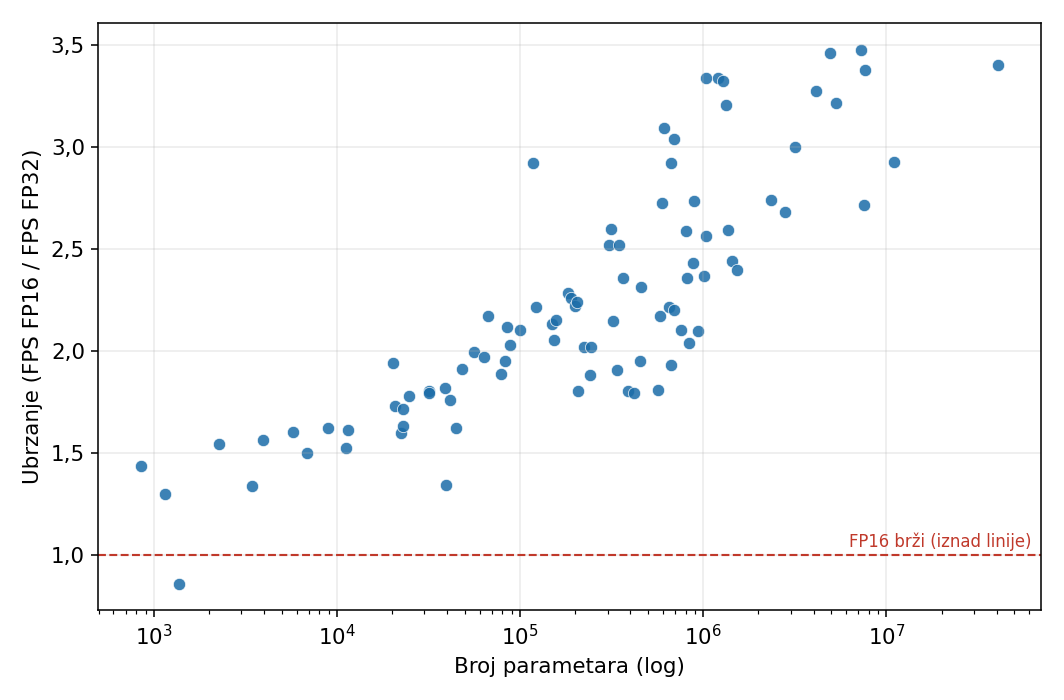
\includegraphics[width=0.6\textwidth]{images/fp16_vs_fp32_speed_diff_480p.png}
	\caption{Ubrzanje FP16 u odnosu na FP32 (odnos broja frejmova u sekundi) u zavisnosti od broja parametara modela, za video rezolucije 480p i uvećanje $\times2$. Tačke iznad isprekidane linije označavaju modele kod kojih je FP16 brži.}
	\label{fig:fp16_vs_fp32_speed_diff}
\end{figure}
Pošto FP16 praktično ne menja kvalitet rekonstrukcije, a znatno ubrzava inferenciju, izabrana je kao podrazumevana preciznost u svim daljim merenjima.

%---------------------------------------------------------------

\section{Poređenje arhitektura}
\label{sec:std_quality}

Izvorni radovi uglavnom prikazuju jednu ili dve konfiguracije svake arhitekture, a efikasnost ocenjuju brojem parametara ili brojem operacija. Međutim, za primenu u realnom vremenu presudno je vreme izvršavanja, a model se ne bira prema najboljem kvalitetu koji arhitektura može da postigne, već prema kvalitetu koji postiže unutar raspoloživog vremenskog budžeta. Zato je svaka arhitektura trenirana u većem broju konfiguracija različite dubine i širine, označenih sa $B/n_f$, gde je $B$ broj blokova, a $n_f$ broj kanala konvolucionih slojeva. Cilj poređenja je da se utvrdi kako se kvalitet i brzina arhitektura menjaju sa njihovom veličinom, koje osobine arhitekture određuju brzinu i koliki se kvalitet može postići uz zadatu minimalnu brzinu.

Sva poređenja u ovom poglavlju odnose se na modele trenirane za uvećanje $\times2$. Kvalitet je ocenjen na validacionom delu skupa DIV2K, a brzina je izmerena postupkom opisanim u poglavlju~\ref{sec:brzina}, za LR ulaz rezolucije $854\times480$ piksela (u daljem tekstu FPS 480p). Poređenje obuhvata arhitekture opisane u poglavlju~\ref{sec:arhitekture}.

\subsection{Kvalitet u odnosu na interpolaciju}

Pre međusobnog poređenja arhitektura potrebno je utvrditi koliko neuronski modeli poboljšavaju rezultat u odnosu na klasične interpolacijske metode, koje plejeri uobičajeno koriste za uvećanje slike. Tabela~\ref{tab:results_best_models} prikazuje interpolacijske metode i, za svaku arhitekturu, najveću treniranu konfiguraciju. Te vrednosti ne predstavljaju najbolji kvalitet koji arhitektura može da postigne, već gornju granicu u ispitanih konfiguracija. Zato služe za procenu raspona poboljšanja u odnosu na interpolaciju, a ne za rangiranje arhitektura, koje se međusobno porede u narednim odeljcima, u zavisnosti od veličine i brzine.

\begin{table}[H]
	\centering
	\begingroup
	\small
	\setlength{\tabcolsep}{3.5pt}
	\renewcommand{\arraystretch}{1.15}
	\newcommand*{\dlt}[1]{\textcolor{gray}{#1}}
	\begin{tabular}{@{}lrrrrrr@{}}
		\toprule
		Model & \shortstack{PSNR $\uparrow$} & \dlt{\shortstack{$\Delta$PSNR}} & \qquad SSIM $\uparrow$ & \dlt{$\Delta$SSIM} & \qquad LPIPS $\downarrow$ & \dlt{$\Delta$LPIPS} \\
		\midrule
		Nearest & 29,25 & \dlt{$-$1,79} & 0,8727 & \dlt{$-$0,0204} & 0,1558 & \dlt{$-$0,0305} \\
		Bilinear & 29,94 & \dlt{$-$1,10} & 0,8687 & \dlt{$-$0,0244} & 0,2290 & \dlt{$+$0,0427} \\
		Bicubic & 31,04 & \dlt{0,00} & 0,8931 & \dlt{0,0000} & 0,1863 & \dlt{0,0000} \\
		Lanczos & 31,51 & \dlt{$+$0,46} & 0,9009 & \dlt{$+$0,0078} & 0,2053 & \dlt{$+$0,0190} \\
		\midrule
		SRCNN & 32,40 & \dlt{$+$1,35} & 0,9159 & \dlt{$+$0,0228} & 0,1360 & \dlt{$-$0,0503} \\
		VDSR & 34,04 & \dlt{$+$3,00} & 0,9329 & \dlt{$+$0,0398} & 0,0930 & \dlt{$-$0,0933} \\
		EDSR & 34,40 & \dlt{$+$3,35} & 0,9357 & \dlt{$+$0,0426} & 0,0884 & \dlt{$-$0,0979} \\
		IMDN & 34,27 & \dlt{$+$3,22} & 0,9345 & \dlt{$+$0,0414} & 0,0916 & \dlt{$-$0,0947} \\
		RFDN & 34,48 & \dlt{$+$3,44} & 0,9362 & \dlt{$+$0,0431} & 0,0907 & \dlt{$-$0,0956} \\
		ABPN & 34,03 & \dlt{$+$2,98} & 0,9323 & \dlt{$+$0,0392} & 0,0930 & \dlt{$-$0,0933} \\
		FastEDSR & 34,19 & \dlt{$+$3,15} & 0,9339 & \dlt{$+$0,0408} & 0,0916 & \dlt{$-$0,0947} \\
		\bottomrule
	\end{tabular}
	\endgroup
	\caption{Kvalitet interpolacijskih metoda i najvećih treniranih konfiguracija arhitektura. Kolone $\Delta$ prikazuju razliku u odnosu na bikubnu interpolaciju.}
	\label{tab:results_best_models}
\end{table}

Svi neuronski modeli nadmašuju interpolacijske metode prema sve tri metrike. Već SRCNN, sa približno $20$ hiljada parametara, povećava PSNR za $0{,}89$ dB u odnosu na Lanczos, interpolacijsku metodu sa najvišim PSNR-om, a LPIPS smanjuje za $0{,}05$ u odnosu na bikubnu interpolaciju. Najveće konfiguracije ostalih arhitektura povećavaju PSNR za $2{,}9$ do $3{,}4$ dB u odnosu na bikubnu interpolaciju, a LPIPS smanjuju približno dvostruko, na $0{,}088$ do $0{,}093$. Međusobne razlike tih konfiguracija, najviše $0{,}46$ dB, znatno su manje od njihove prednosti nad interpolacijom.

Poredak metoda zavisi i od izabrane metrike. Lanczos postiže viši PSNR i SSIM od bikubne interpolacije, ali ima lošiji LPIPS, a interpolacija najbližim susedom ima čak niži LPIPS od bikubne i bilinearne interpolacije, iako je vizuelno najgrublja. LPIPS, dakle, strože kažnjava zamućenje nego blokovske artefakte. Nijedna metrika zato sama ne opisuje kvalitet rekonstrukcije, pa se ocena zasniva na zajedničkom razmatranju metrika i vizuelnih primera.

Slika~\ref{fig:compare_standard_best_models} prikazuje rekonstrukciju detalja sa slike 0879 iz validacionog dela skupa DIV2K. Bilinearna, bikubna i Lanczos interpolacija zamućuju konture lukova i okvira prozora, a interpolacija najbližim susedom daje stepenaste ivice. Neuronski modeli rekonstruišu oštrije i kontinualnije ivice. Izuzetak je delimično SRCNN, kod koga su konture oštrije nego kod interpolacije, ali sa vidljivim artefaktima. Razlike između ostalih neuronskih modela na ovom primeru su teško uočljive.

\begin{figure}[H]
	\centering
	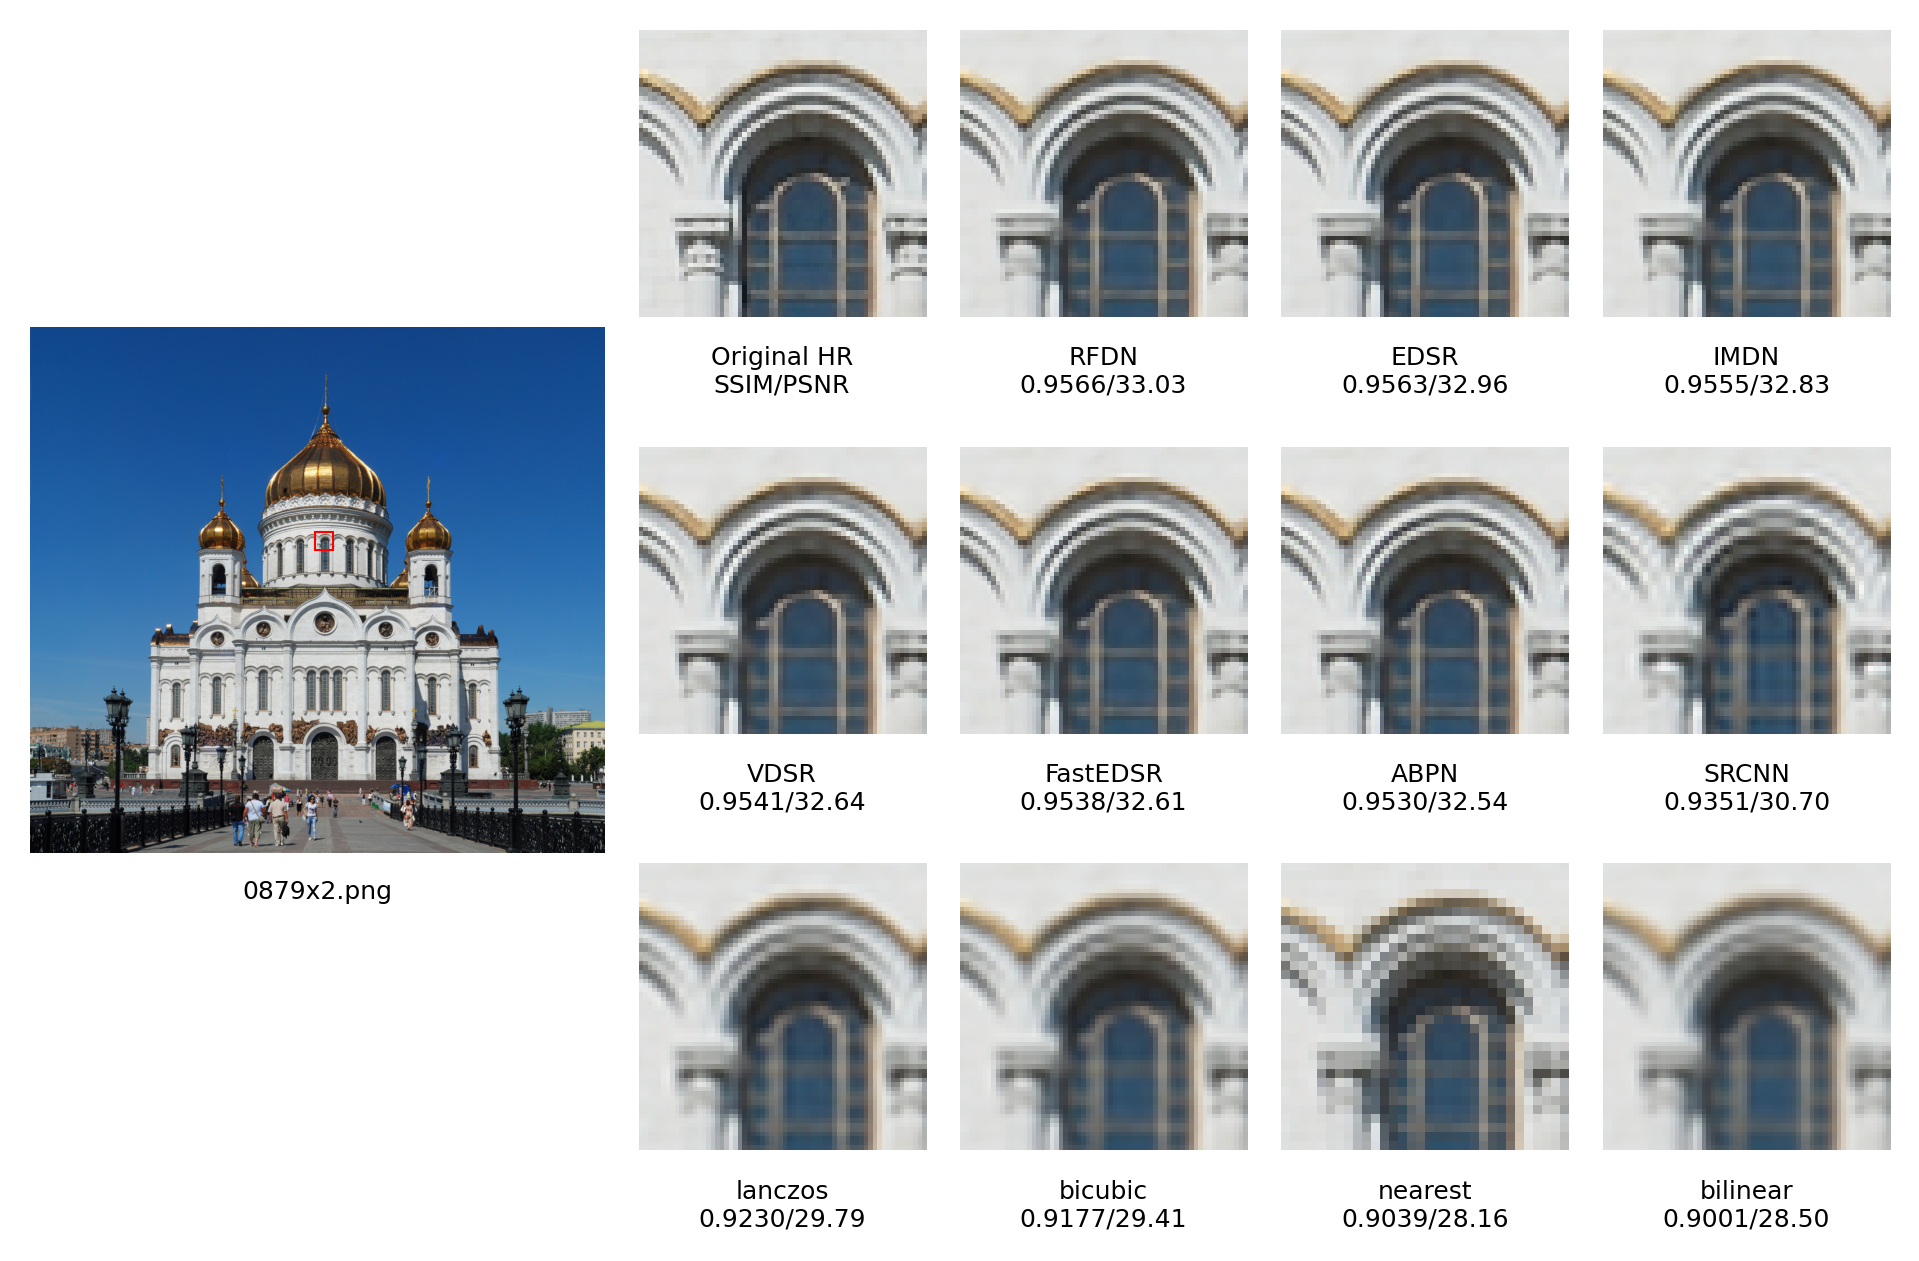
\includegraphics[width=\textwidth]{images/comparison_best_models_0879x2.png}
	\caption{Vizuelno poređenje interpolacijskih metoda i najvećih treniranih konfiguracija arhitektura pri uvećanju $\times2$ na slici 0879 iz skupa DIV2K.}
	\label{fig:compare_standard_best_models}
\end{figure}

\subsection{Odnos kvaliteta i veličine modela}

Tabela~\ref{tab:param_bins} izdvaja najbolje konfiguracije arhitektura po metrici, unutar svakog opsega broja parametara. Oznake K i M predstavljaju hiljade i milione parametara.

\begin{table}[H]
	\centering
	\small
	\setlength{\tabcolsep}{5pt}
	\begin{tabular}{@{}llll@{}}
		\toprule
		Opseg parametara & Najbolji PSNR $\uparrow$ & Najbolji SSIM $\uparrow$ & Najbolji LPIPS $\downarrow$ \\
		\midrule
		$<$10\,K & $\text{FastEDSR}_{\text{4/8}}$ (32,74) & $\text{FastEDSR}_{\text{4/8}}$ (0,920) & $\text{ABPN}_{\text{2/16}}$ (0,127) \\
		10\,K-50\,K & $\text{VDSR}_{\text{5/32}}$ (33,35) & $\text{VDSR}_{\text{5/32}}$ (0,926) & $\text{VDSR}_{\text{5/32}}$ (0,105) \\
		50\,K-200\,K & $\text{VDSR}_{\text{5/64}}$ (33,64) & $\text{VDSR}_{\text{5/64}}$ (0,929) & $\text{ABPN}_{\text{8/48}}$ (0,102) \\
		200\,K-500\,K & $\text{VDSR}_{\text{10/64}}$ (33,84) & $\text{VDSR}_{\text{10/64}}$ (0,931) & $\text{FastEDSR}_{\text{4/64}}$ (0,096) \\
		500\,K-1\,M & $\text{RFDN}_{\text{2/96}}$ (33,90) & $\text{RFDN}_{\text{2/96}}$ (0,931) & $\text{ABPN}_{\text{4/128}}$ (0,095) \\
		1\,M-3\,M & $\text{RFDN}_{\text{4/128}}$ (34,25) & $\text{RFDN}_{\text{4/128}}$ (0,934) & $\text{ABPN}_{\text{4/256}}$ (0,093) \\
		$>$3\,M & $\text{RFDN}_{\text{4/256}}$ (34,48) & $\text{RFDN}_{\text{4/256}}$ (0,936) & $\text{EDSR}_{\text{32/256}}$ (0,088) \\
		\bottomrule
	\end{tabular}
	\caption{Najbolje konfiguracije arhitektura po metrici i opsegu broja parametara}
	\label{tab:param_bins}
\end{table}

U opsezima od $10$ do $500$ hiljada parametara VDSR daje najbolji PSNR i SSIM. Iznad tog opsega za PSNR i SSIM prednjači RFDN, dok za LPIPS uglavnom najbolji odnos ima ABPN.

Slika~\ref{fig:quality_vs_params} grafički prikazuje odnos LPIPS metrike i broja parametara. Za svaku arhitekturu prikazan je samo njen Pareto front, odnosno konfiguracije za koje ne postoji manja konfiguracija iste arhitekture sa barem jednako dobrim kvalitetom. Da bi grafici bili pregledniji, arhitekture su raspoređene u tri panela, prema tome u kom prostoru rade konvolucije i šta mreža koristi pored njih. VDSR radi nad bikubno uvećanom slikom. IMDN i RFDN rade u LR prostoru, a njihovi blokovi pored konvolucija razdvajaju i spajaju kanale i koriste mehanizme pažnje. ABPN i FastEDSR takođe rade u LR prostoru, ali ih čine samo konvolucije, aktivacije i sabiranja, a izlaz je rezidual koji se dodaje na ulaz uvećan jednostavnom interpolacijom. EDSR je prikazan u svakom panelu kao zajednička referenca. On radi u LR prostoru sa istim jednostavnim operacijama kao ABPN i FastEDSR, ali ne predviđa rezidual nad uvećanim ulazom, pa se uz VDSR vidi šta donosi rad u LR prostoru, uz IMDN i RFDN koliko koštaju destilacija i pažnja, a uz ABPN i FastEDSR šta donosi rezidual nad uvećanim ulazom. Ista podela koristi se i na graficima u narednim odeljcima.

\begin{figure}[H]
	\centering
	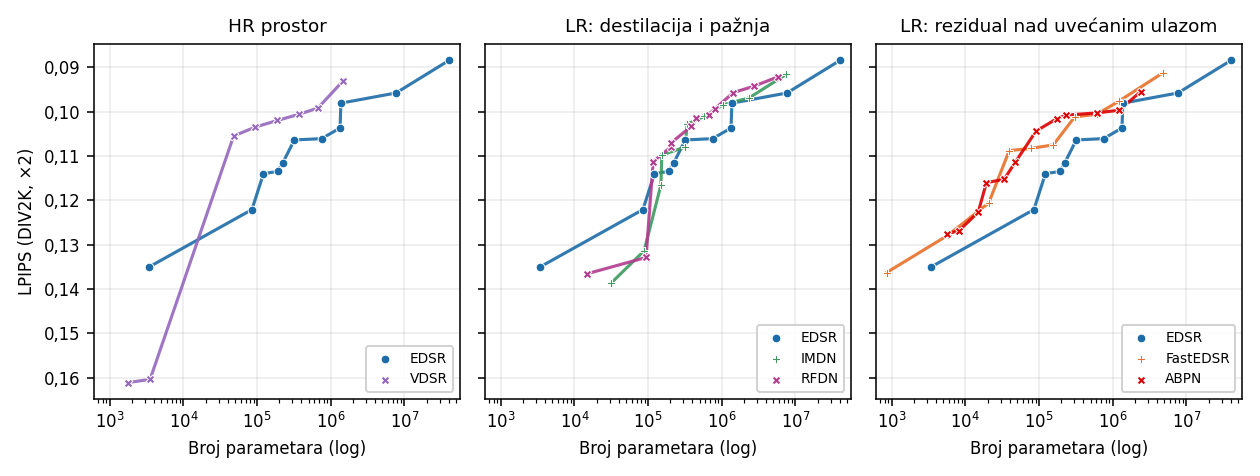
\includegraphics[width=\textwidth]{images/LPIPS_vs_params_panels.png}
	\caption{LPIPS kvalitet rekonstrukcije u funkciji broja parametara. LPIPS vertikalna osa je invertovana, tako da bolji kvalitet odgovara višem položaju. Horizontalna osa je logaritamska.}
	\label{fig:quality_vs_params}
\end{figure}

VDSR ima dosta dobar odnos kvaliteta i broja parametara, ali tek nakon približno $50$ hiljada parametara. Rad nad uvećanom slikom ne povećava broj parametara, već samo broj izračunavanja, pa je VDSR efikasan po parametrima. U grupi sa destilacijom i pažnjom IMDN i RFDN su međusobno približni, dok su tek od $100$ hiljada parametara uporedivi sa EDSR-om. U grupi sa rezidualom nad uvećanim ulazom FastEDSR i ABPN su bolji od EDSR-a.

\subsection{Odnos veličine i brzine modela}

Broj parametara, međutim, ne određuje brzinu inferencije. Slika~\ref{fig:fps_vs_params} prikazuje odnos brzine i broja parametara, uz Pareto front po arhitekturi, odnosno najbrže konfiguracije za datu veličinu: za konfiguraciju na frontu ne postoji konfiguracija iste arhitekture sa barem jednako mnogo parametara koja je barem jednako brza.

\begin{figure}[H]
	\centering
	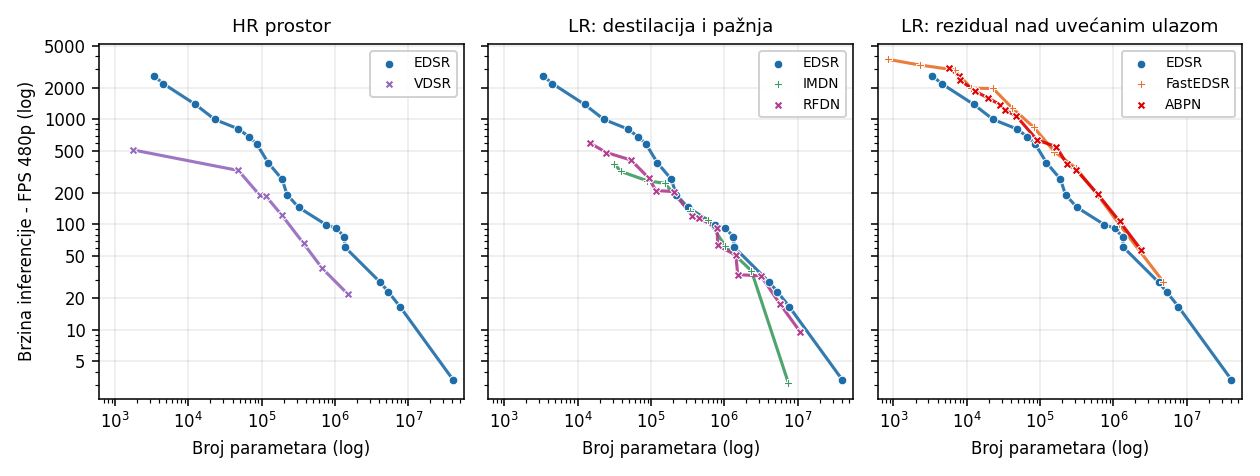
\includegraphics[width=\textwidth]{images/FPS_vs_params_panels.png}
	\caption{Brzina inferencije u odnosu na broj parametara. Obe ose su logaritamske}
	\label{fig:fps_vs_params}
\end{figure}

VDSR, koji ima najbolji odnos kvaliteta i broja parametara, ovde je najsporiji, jer sve konfiguracije izvršava nad bikubno uvećanom slikom, odnosno nad $s^2=4$ puta više piksela od arhitektura koje rade u LR prostoru. VDSR, IMDN i RFDN pokazuju pad brzine po parametrima nad konfiguracijama ispod $100$ hiljada parametara. U grupi sa rezidualom nad uvećanim ulazom linije FastEDSR-a i ABPN-a nalaze se iznad linije EDSR-a u celom opsegu i međusobno se gotovo poklapaju. Iznad približno milion parametara razlike između arhitektura se smanjuju, jer vreme izvršavanja tada sve više određuju same konvolucije. Dobar odnos kvaliteta i broja parametara zato ne mora značiti i veliku brzinu izvršavanja, što je za rad u realnom vremenu presudno.

\subsection{Odnos kvaliteta i brzine modela}

Za izbor modela za video-plejer najkorisnije je pitanje koliki se kvalitet može postići uz zadatu minimalnu brzinu. Za svaki prag FPS-a zato se posmatraju svi modeli koji ga dostižu i među njima se bira najbolji. Slika~\ref{fig:fps_thr_LPIPS} prikazuje odnos kvaliteta i brzine grafički. Tabele~\ref{tab:fps_thr_SSIM} i~\ref{tab:fps_thr_LPIPS} ga prikazuju brojčano, kroz najbolji rezultat svake arhitekture za svaki prag.

\begin{figure}[H]
	\centering
	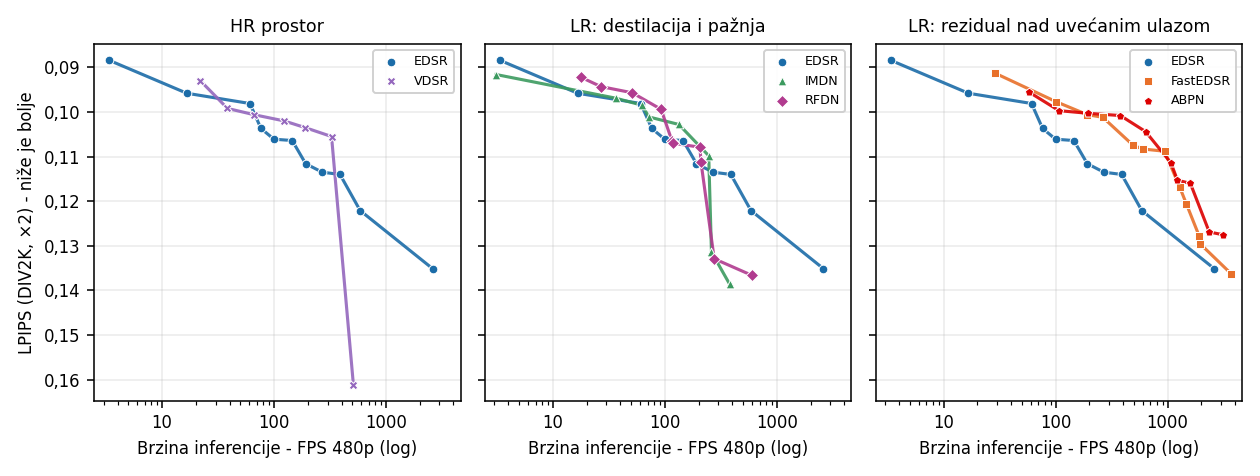
\includegraphics[width=\textwidth]{images/fps_thresholds_LPIPS_panels_single.png}
	\caption{Pareto front po arhitekturi: LPIPS u funkciji brzine inferencije. Vertikalna osa je invertovana, tako da bolji kvalitet odgovara višem položaju.}
	\label{fig:fps_thr_LPIPS}
\end{figure}

\begin{table}[H]
	\centering
	\small
	\setlength{\tabcolsep}{5pt}
	\begin{tabular}{@{}lrrrrrrr@{}}
		\toprule
		FPS & $\geq$20 & $\geq$30 & $\geq$60 & $\geq$80 & $\geq$120 & $\geq$250 & $\geq$500 \\
		\midrule
		VDSR & 0,9329 & 0,9307 & 0,9307 & 0,9290 & 0,9290 & 0,9265 & 0,9090 \\
		EDSR & 0,9326 & 0,9326 & \textbf{0,9326} & 0,9278 & 0,9274 & 0,9244 & 0,9213 \\
		IMDN & 0,9320 & 0,9320 & 0,9307 & 0,9293 & 0,9277 & 0,9190 & --- \\
		RFDN & \textbf{0,9340} & \textbf{0,9327} & 0,9311 & 0,9304 & 0,9259 & 0,9183 & 0,9114 \\
		FastEDSR & 0,9333 & 0,9320 & 0,9320 & \textbf{0,9320} & 0,9296 & \textbf{0,9296} & 0,9259 \\
		ABPN & 0,9319 & 0,9319 & 0,9301 & 0,9301 & \textbf{0,9301} & 0,9278 & \textbf{0,9262} \\
		\bottomrule
	\end{tabular}
	\caption{Najbolji SSIM $\uparrow$ koji svaka arhitektura postiže uz zadatu minimalnu brzinu. Najbolja vrednost u koloni je podebljana.}
	\label{tab:fps_thr_SSIM}
\end{table}

\begin{table}[H]
	\centering
	\small
	\setlength{\tabcolsep}{8pt}
	\begin{tabular}{@{}lrrrrrrr@{}}
		\toprule
		FPS & $\geq$20 & $\geq$30 & $\geq$60 & $\geq$80 & $\geq$120 & $\geq$250 & $\geq$500 \\
		\midrule
		VDSR & 0,093 & 0,099 & 0,101 & 0,102 & 0,102 & 0,105 & 0,161 \\
		EDSR & 0,098 & 0,098 & 0,098 & 0,106 & 0,106 & 0,114 & 0,122 \\
		IMDN & 0,097 & 0,097 & 0,099 & 0,103 & 0,103 & 0,131 & --- \\
		RFDN & 0,094 & 0,096 & 0,099 & 0,099 & 0,108 & 0,133 & 0,137 \\
		FastEDSR & \textbf{0,091} & 0,098 & \textbf{0,098} & \textbf{0,098} & 0,101 & 0,101 & 0,108 \\
		ABPN & 0,096 & \textbf{0,096} & 0,100 & 0,100 & \textbf{0,100} & \textbf{0,101} & \textbf{0,104} \\
		\bottomrule
	\end{tabular}
	\caption{Najbolji LPIPS $\downarrow$ koji svaka arhitektura postiže uz zadatu minimalnu brzinu. Najbolja vrednost u koloni je podebljana.}
	\label{tab:fps_thr_LPIPS}
\end{table}

Iz slike i tabela izdvajaju se tri zapažanja. Prvo, kvalitet se sporo menja sa zahtevom za brzinom. Uz najmanje $30$ FPS najbolji model postiže SSIM $0{,}9327$, a uz najmanje $250$ FPS SSIM $0{,}9296$. Približno osam puta veća brzina smanjuje tako SSIM za $0{,}0031$, što je manje od desetine poboljšanja koje modeli donose u odnosu na bikubnu interpolaciju (tabela~\ref{tab:results_best_models}). Najbolji LPIPS pri tome raste sa $0{,}096$ na $0{,}101$.

Drugo, uz najmanje $30$ FPS SSIM najboljih konfiguracija svih arhitektura razlikuje se za najviše $0{,}002$, ali arhitekture iz prve dve grupe ne zadržavaju kvalitet pri većim brzinama. Linije IMDN-a i RFDN-a prate EDSR do približno $200$ FPS, a zatim naglo padaju, što odgovara gornjoj granici njihove brzine. Uz najmanje $250$ FPS njihov najbolji SSIM iznosi oko $0{,}919$, naspram $0{,}9296$ kod FastEDSR-a, a LPIPS oko $0{,}13$, naspram $0{,}101$, dok granicu od $500$ FPS IMDN uopšte ne dostiže. VDSR je između približno $80$ i $300$ FPS bolji od EDSR-a, ali iznad toga naglo gubi kvalitet, jer brže konfiguracije moraju biti veoma plitke. Uz najmanje $250$ FPS VDSR i EDSR zaostaju za FastEDSR-om po SSIM-u za $0{,}003$, odnosno $0{,}005$.

Treće, linije ABPN-a i FastEDSR-a nalaze se iznad skoro cele linije EDSR-a i međusobno su praktično izjednačene, a uz najmanje $80$ FPS najbolji rezultat prema svim metrikama postižu isključivo ove dve arhitekture.

Poređenje arhitektura pokazuje da za rad u realnom vremenu najbolji odnos kvaliteta i brzine imaju jednostavne arhitekture koje rade u LR prostoru i predviđaju samo rezidual nad interpoliranim ulazom. Rad u LR prostoru smanjuje broj piksela nad kojima se izvršavaju konvolucije $s^2$ puta, zbog čega je VDSR, iako najefikasniji po broju parametara, najsporiji. Destilacija i pažnja kod IMDN-a i RFDN-a smanjuju broj parametara, ali dodatne operacije razdvajanja i spajanja kanala i mehanizmi pažnje produžavaju izvršavanje, pa ove arhitekture pri većim brzinama gube kvalitet. FastEDSR i ABPN objedinjuju dva svojstva: čine ih samo konvolucije, aktivacije i sabiranja, i predviđaju samo rezidual nad interpoliranim ulazom. Prvo svojstvo daje najbrže izvršavanje za dati broj parametara, a drugo omogućava da i male konfiguracije zadrže dobar kvalitet. Zato su ovakve arhitekture najpogodnije za superrezoluciju u video-plejeru.

\section{Višeskalni modeli}
\label{sec:viseskalni}

Pored modela treniranih za pojedinačne faktore uvećanja, implementirane su i višeskalne varijante, koje u okviru jedne mreže podržavaju faktore $\times2$, $\times3$ i $\times4$. Od skale zavisi samo mali deo mreže, dok je ostatak zajednički za sve faktore. Inspiracija za ovakav pristup bila je arhitektura MDSR, opisana u odeljku~\ref{sec:mdsr}.

Kod arhitektura SRCNN i VDSR za to nije potrebna promena strukture, jer se ulazna slika unapred interpolira na ciljnu rezoluciju, pa mreža uvek radi u HR prostoru. EDSR, IMDN, RFDN, ABPN i FastEDSR, sa druge strane, uvećavaju sliku unutar same mreže sub-pikselnom konvolucijom, čiji broj izlaznih kanala i PixelShuffle zavise od faktora uvećanja. Njihove višeskalne varijante zato imaju zasebnu sub-pikselnu konvoluciju za svaki faktor, dok je ostatak mreže zajednički. Primer za višeskalni FastEDSR model dat je na slici~\ref{fig:diagram_FastEDSR_Multiscale}.

\begin{figure}[H]
	\centering
	\resizebox{0.9\textwidth}{!}{\begin{tikzpicture}[
	font=\sffamily\small,
	node distance=5mm,
	>=stealth,
	blk/.style={draw, rounded corners=3pt, align=center, minimum height=10mm, inner sep=0.5mm},
	io/.style={blk, fill=gray!15, draw=gray!60, minimum width=10mm},
	conv/.style={blk, fill=cyan!20, draw=cyan!50, minimum width=20mm},
	res/.style={blk, fill=green!50!black!15, draw=green!50!black!60, minimum width=22mm},
	ub/.style={blk, fill=yellow!45!orange!35, draw=orange!50, minimum width=30mm},
	interp/.style={blk, fill=yellow!45!orange!35, draw=orange!50, minimum height=8mm},
	dec/.style={diamond, aspect=1, draw, rounded corners=2pt, align=center, font=\sffamily\scriptsize, inner sep=0.5mm, minimum size=15mm},
	op/.style={circle, draw=gray!50, fill=gray!20, minimum size=7mm, inner sep=0pt}
	]
	% --- trup ---
	\node[io] (lr) {LR};
	\node[conv, right=8mm of lr] (m1) {Conv 3\,\texttimes\,3};
	\node[right=3mm of m1] (dots) {$\cdots$};
	\node[res, right=3mm of dots] (rb2) {ResBlock};

	\draw[->] (lr) -- (m1);
	\draw[->] (m1) -- (dots);
	\draw[->] (dots) -- (rb2);

	% --- izbor skale (kolona rombova) ---
	\node[dec, right=8mm of rb2] (d2) {skala\\\texttimes2};
	\node[dec] (d3) at ($(d2)+(0,-20mm)$) {skala\\\texttimes3};
	\node[dec] (d4) at ($(d2)+(0,-40mm)$) {skala\\\texttimes4};
	\draw[->] (rb2) -- (d2);
	\draw[->] (d2) -- (d3);
	\draw[->] (d3) -- (d4);

	% --- blokovi za uvećanje kao pojedinačni čvorovi ---
	\foreach \s in {2,3,4} {
		\node[ub, right=8mm of d\s] (u\s) {Sub-pixel Conv(\s)};
		\draw[->] (d\s) -- (u\s);
	}

	% --- spajanje grana ---
	\coordinate (merge) at ($(u2.east)+(6mm,0)$);
	\node[op, right=8mm of merge] (add) {$+$};
	\node[io, right=of add] (sr) {SR};
	\draw[->] (u2.east) -- (add.west);
	\draw[->] (u4.east) -| (merge);
	\draw (u3.east) -- (merge |- u3);
	\draw[->] (add) -- (sr);

	% --- bilinearna osnova (iznad trupa) ---
	\coordinate (split) at ($(lr.east)!0.5!(m1.west)$);
	\coordinate (btop) at ($(split)+(0,16mm)$);
	\node[interp, minimum width=40mm] (bil) at ($(btop)!0.5!(add.north |- btop)$) {Bilinearna interpolacija};
	\draw[->] (split) |- (bil.west);
	\draw[->] (bil.east) -| (add.north);
\end{tikzpicture}
}
	\caption{Arhitektura višeskalnog FastEDSR modela.}
	\label{fig:diagram_FastEDSR_Multiscale}
\end{figure}

Faktor uvećanja prosleđuje se modelu kao dodatni argument i određuje koja se sub-pikselna konvolucija izvršava, pa se pri jednoj inferenciji koristi samo grana izabrane skale. Pri treniranju se za svaki mini-batch nasumično bira jedan od tri faktora, a zatim se koriste parovi LR i HR isečaka za taj faktor. Zajednički deo mreže tako uči na primerima svih skala, dok se sub-pikselna konvolucija pojedinačne skale ažurira samo kada je ta skala izabrana.

Da bi se proverilo da li zajednički deo mreže umanjuje kvalitet, svaki višeskalni model upoređen je sa modelima iste arhitekture i konfiguracije $B/n_f$ koji su trenirani samo za jedan faktor uvećanja, u daljem tekstu namenskim modelima. Tabela~\ref{tab:multiscale_DIV2K} prikazuje rezultate obe grupe, usrednjene po svim konfiguracijama za svaki faktor uvećanja.

\begin{table}[H]
	\centering
	\begingroup
	\small
	\setlength{\tabcolsep}{8pt}
	\renewcommand{\arraystretch}{1.15}
	\begin{tabular}{@{}lcccccc@{}}
		\toprule
		Faktor & \multicolumn{2}{c}{PSNR $\uparrow$} & \multicolumn{2}{c}{SSIM $\uparrow$} & \multicolumn{2}{c}{LPIPS $\downarrow$} \\
		\cmidrule(lr){2-3}\cmidrule(lr){4-5}\cmidrule(lr){6-7}
		& namenski & multi & namenski & multi & namenski & multi \\
		\midrule
		$\times2$ & 33,26 & \textbf{33,27} & 0,9250 & \textbf{0,9252} & 0,1108 & \textbf{0,1085} \\
		$\times3$ & 29,59 & \textbf{29,67} & 0,8481 & \textbf{0,8497} & \textbf{0,2496} & 0,2501 \\
		$\times4$ & 27,73 & \textbf{27,86} & 0,7859 & \textbf{0,7893} & 0,3384 & \textbf{0,3364} \\
		\bottomrule
	\end{tabular}
	\endgroup
	\caption{Prosečan kvalitet namenskih i višeskalnih modela iste konfiguracije na skupu DIV2K, po faktoru uvećanja.}
	\label{tab:multiscale_DIV2K}
\end{table}

Višeskalni modeli za sva tri faktora postižu u proseku približno jednak ili nešto bolji rezultat po svim metrikama. Više faktora uvećanja može se, dakle, objediniti u jednom modelu bez gubitka kvaliteta, umesto da se za svaki faktor trenira i održava zasebna mreža. To je posebno korisno u video-plejeru, gde potreban faktor zavisi od rezolucije video-zapisa i ekrana.

\section{Superrezolucija JPEG-kompresovanih slika}
\label{sec:jpeg}

U prethodnim eksperimentima slike niske rezolucije formirane su bikubnim smanjivanjem odgovarajućih HR slika, bez uvođenja dodatne JPEG kompresije. Referentne slike čuvane su u PNG formatu, čime se prilikom njihovog čuvanja ne uvode dodatni gubici. Međutim, u praktičnim uslovima ulazni sadržaj je često čuvan uz kompresiju sa gubicima. U tom slučaju, pored gubitka prostornih detalja usled smanjenja rezolucije, u slici su prisutni i kompresioni artefakti. Zbog toga je dodatno ispitano ponašanje modela kada su LR ulazi kompresovani JPEG algoritmom \cite{JPEG}. Ovakav scenario je značajan i sa stanovišta primene superrezolucije nad kompresovanim video sadržajem.

Deo modela treniran je tako što je nakon formiranja LR slike primenjena dodatna JPEG kompresija, sa uniformno nasumičnim kvalitetom u opsegu od 20 do 95, dok je odgovarajuća HR slika zadržana kao referentni izlaz. Na ovaj način model istovremeno uči povećanje prostorne rezolucije i ublažavanje artefakata nastalih kompresijom. Sličan pristup, sa JPEG kompresijom kao delom modela degradacije pri formiranju trening parova, koriste i radovi \cite{BSRGAN, RealESRGAN}. Arhitektura modela pri tome nije menjana, jedina razlika u odnosu na bazne modele nalazi se u postupku pripreme podataka za treniranje.

Za evaluaciju je korišćen modifikovani test skup DIV2K, gde su LR slike dodatno JPEG-kompresovane, pri čemu je vrednost JPEG kvaliteta birana iz opsega od 20 do 100 prema ravnomernoj raspodeli. Na taj način test skup obuhvata različite stepene kompresije. Tabela~\ref{tab:jpeg_DIV2K_jpeg} prikazuje rezultate baznih modela i odgovarajućih modela treniranih sa JPEG degradacijom za faktor uvećanja $\times2$.

\begin{table}[H]
	\centering
	\small
	\setlength{\tabcolsep}{8pt}
	 \begin{tabular}{lcccccc}
		\toprule
		Model & \multicolumn{2}{c}{PSNR $\uparrow$} & \multicolumn{2}{c}{SSIM $\uparrow$} & \multicolumn{2}{c}{LPIPS $\downarrow$} \\
		\cmidrule(lr){2-3}\cmidrule(lr){4-5}\cmidrule(lr){6-7}
		& bazni & jpeg & bazni & jpeg & bazni & jpeg \\
		\midrule
		FastEDSR 4/32 & 28,382 & \textbf{29,108} & 0,804 & \textbf{0,826} & \textbf{0,268} & 0,280 \\
		FastEDSR 4/64 & 28,375 & \textbf{29,332} & 0,804 & \textbf{0,832} & \textbf{0,262} & 0,273 \\
		FastEDSR 4/128 & 28,388 & \textbf{29,543} & 0,804 & \textbf{0,837} & \textbf{0,265} & 0,267 \\
		FastEDSR 4/256 & 28,405 & \textbf{29,635} & 0,805 & \textbf{0,839} & 0,270 & \textbf{0,263} \\
		RFDN 2/128 & 28,366 & \textbf{29,408} & 0,804 & \textbf{0,842} & 0,265 & \textbf{0,255} \\
		\bottomrule
	\end{tabular}
	\caption{Poređenje JPEG modela}
	\label{tab:jpeg_DIV2K_jpeg}
\end{table}

Rezultati pokazuju jasno poboljšanje PSNR i SSIM metrika kod modela treniranih sa JPEG degradacijom. Prosečno povećanje PSNR-a iznosi $1{,}022$ dB, dok se SSIM u proseku povećava za oko $0{,}031$. Ovakav rezultat pokazuje da uključivanje JPEG degradacije tokom treniranja omogućava modelu da se bolje prilagodi kompresovanim ulazima i efikasnije ublaži prisutne kompresione artefakte. Vizuelni primer se može videti na slici~\ref{fig:primer_jpg}.


\begin{figure}[H]
	\centering
	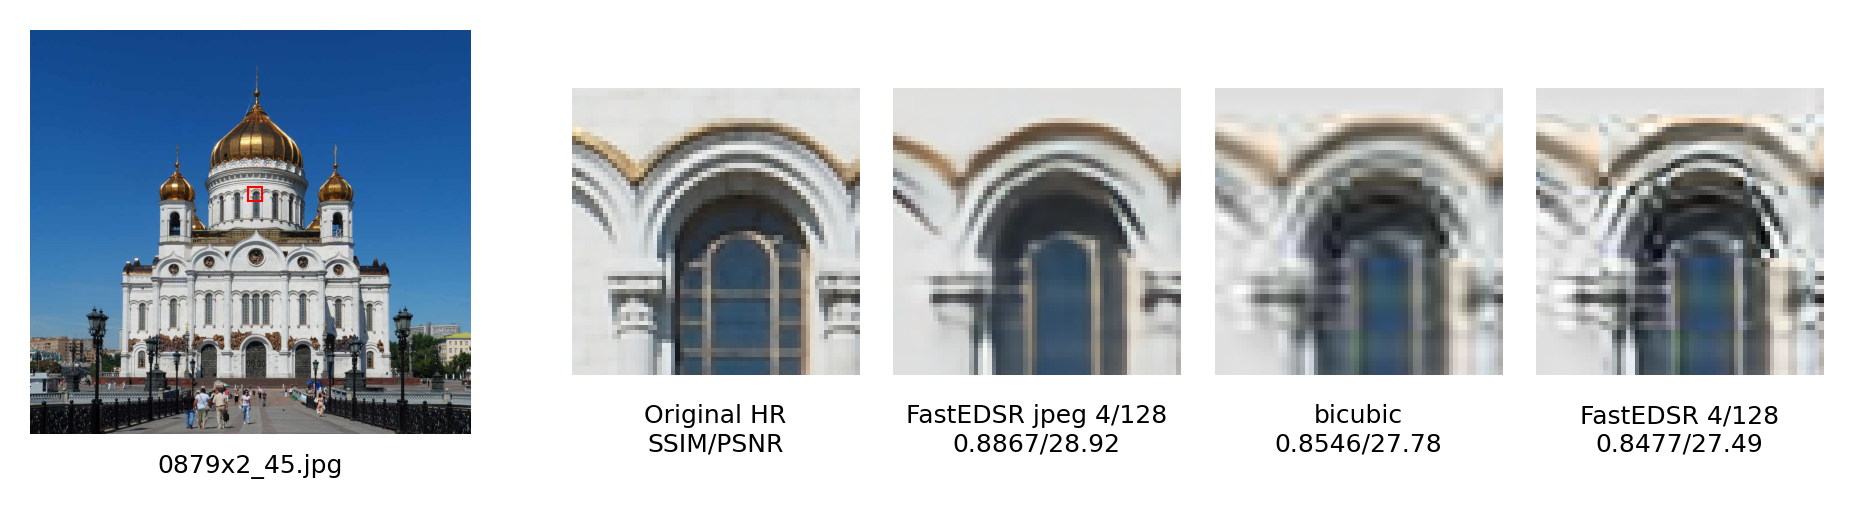
\includegraphics[width=\textwidth]{images/comparison_jpeg_0879x4_45.png}
	\caption{Vizuelno poređenje rekonstrukcije JPEG-kompresovane slike pri faktoru uvećanja $\times2$ za bazni model, model treniran sa JPEG degradacijom i bikubnu interpolaciju.}
	\label{fig:primer_jpg}
\end{figure}

Sa druge strane, poboljšanje PSNR-a i SSIM-a nije praćeno jednakim poboljšanjem perceptualne metrike. Prosečna vrednost LPIPS-a povećava se za približno $0{,}0016$, što predstavlja blago pogoršanje prema ovoj metrici. Vizuelnom analizom uočeno je da su rekonstruisane slike modela treniranih sa JPEG degradacijom vidljivo zamućene. Model prilikom uklanjanja kompresionih artefakata može istovremeno potisnuti deo visokofrekventnih detalja, što dovodi do blagog zamućenja i može uticati na LPIPS.

Zbog toga je ispitan i postupak u kome se tokom treniranja dodatno izoštrava referentna HR slika. LR ulaz formira se pre ovog koraka, tako da izoštravanje ne menja ulaz modela, već isključivo ciljnu sliku koju mreža treba da rekonstruiše. Na taj način model se tokom treniranja podstiče da generiše izraženije ivice i fine detalje, bez potrebe za uvođenjem zasebnog koraka izoštravanja tokom inferencije. Izoštravanje referentnih slika tokom treniranja koristi i Real-ESRGAN \cite{RealESRGAN}.

Pri vizuelnom poređenju izlazi ovako treniranih modela delovali su oštrije od izlaza odgovarajućih modela treniranih bez izoštravanja referentnih slika. Uticaj ovog postupka dodatno je analiziran pomoću SSIM i LPIPS metrika na JPEG-kompresovanom validacionom skupu DIV2K za faktor uvećanja $\times2$. Rezultati su prikazani u tabeli~\ref{tab:jpeg_DIV2K_jpeg_vs_s_2}, gde oznaka \textit{jpeg} predstavlja model treniran sa JPEG degradacijom, dok \textit{jpeg\_s} označava varijantu kod koje je dodatno izoštravana referentna HR slika.

\begin{table}[H]
	\centering
	\small
	\setlength{\tabcolsep}{8pt}
	\begin{tabular}{lcccccc}
		\toprule
		Model & \multicolumn{3}{c}{SSIM $\uparrow$} & \multicolumn{3}{c}{LPIPS $\downarrow$} \\
		\cmidrule(lr){2-4}\cmidrule(lr){5-7}
		& bazni & jpeg & jpeg\_s & bazni & jpeg & jpeg\_s \\
		\midrule
		FastEDSR 4/32 & 0,804 & 0,826 & \textbf{0,829} & \textbf{0,268} & 0,280 & 0,270 \\
		FastEDSR 4/64 & 0,804 & 0,832 & \textbf{0,835} & \textbf{0,262} & 0,273 & 0,263 \\
		FastEDSR 4/128 & 0,804 & 0,837 & \textbf{0,839} & 0,265 & 0,267 & \textbf{0,259} \\
		RFDN 2/128 & 0,804 & 0,842 & \textbf{0,842} & 0,265 & 0,255 & \textbf{0,255} \\
		\bottomrule
	\end{tabular}
	\caption{Poređenje JPEG modela}
	\label{tab:jpeg_DIV2K_jpeg_vs_s_2}
\end{table}

U odnosu na modele trenirane samo sa JPEG degradacijom, korišćenje izoštrenih referentnih slika smanjuje LPIPS u proseku za približno $0{,}007$, dok se SSIM dodatno povećava za približno $0{,}002$. U poređenju sa baznim modelima, JPEG-S varijante zadržavaju znatno viši SSIM, sa prosečnim povećanjem od oko $0{,}032$, i manjim smanjenjem LPIPS vrednosti, u proseku od $0{,}003$, što je praktično jednako vrednosti baznih modela. Na taj način izoštravanje referentnih slika ublažava perceptualni nedostatak uočen kod modela treniranih samo sa JPEG degradacijom, bez potrebe za promenom same arhitekture mreže. Vizuelni primer na slici~\ref{fig:primer_jpg_sharp} ilustruje razliku između posmatranih pristupa.

\begin{figure}[H]
	\centering
	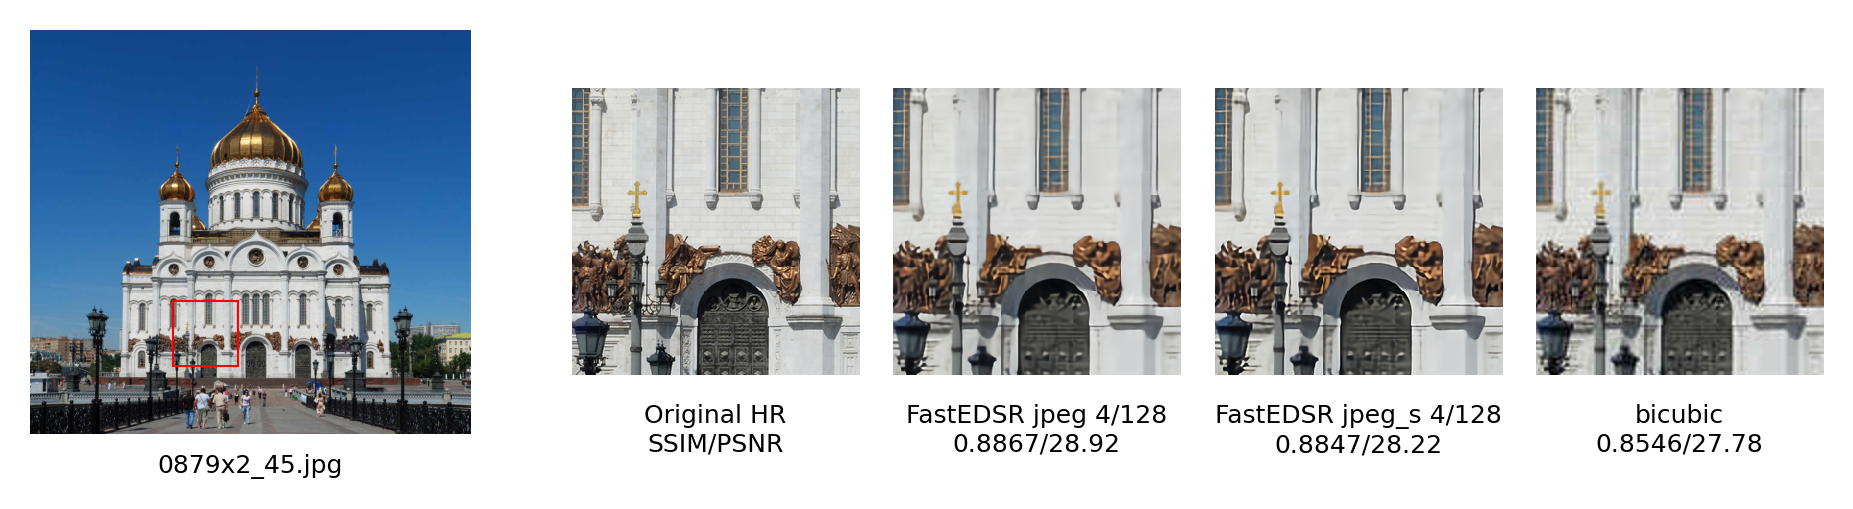
\includegraphics[width=\textwidth]{images/comparison_jpeg_sharp_0879x2_45.png}
	\caption{Vizuelno poređenje rekonstrukcije JPEG-kompresovane slike pri faktoru uvećanja $\times2$ za model treniran sa JPEG degradacijom i varijantu sa dodatno izoštrenom referentnom HR slikom.}
	\label{fig:primer_jpg_sharp}
\end{figure}

%---------------------------------------------------------------

\section{Izvršna okruženja za inferenciju}
\label{sec:izvrsna_okruzenja}

Modeli su trenirani u okruženju PyTorch \cite{PyTorch}, ali u aplikaciji koja obrađuje video-zapis model se izvršava pomoću izvršnog okruženja (engl.\ \textit{runtime}). To je biblioteka koja učitava opis mreže i njene težine i izvršava operacije računskog grafa na izabranom hardveru. Izvršna okruženja razlikuju se po podržanom hardveru i operativnim sistemima, po optimizacijama koje primenjuju i po načinu pokretanja. U ovom radu korišćena su tri: ONNX Runtime, TensorRT i NCNN. Zajednička polazna tačka za sva tri je zapis modela u formatu ONNX, iz kog svako okruženje dalje priprema model na svoj način (slika~\ref{fig:izvrsna_okruzenja}): ONNX Runtime ga učitava neposredno, TensorRT na osnovu njega gradi optimizovani engine za konkretnu grafičku karticu, a za NCNN se model konvertuje u sopstveni format.

\begin{figure}[H]
	\centering
	\resizebox{0.75\textwidth}{!}{\begin{tikzpicture}[
	font=\sffamily\small,
	>=stealth,
	blk/.style={draw, rounded corners=3pt, align=center, minimum height=9mm, inner sep=1.5mm},
	src/.style={blk, fill=gray!15, draw=gray!60, minimum width=20mm},
	fmt/.style={blk, fill=cyan!20, draw=cyan!60, minimum width=18mm},
	rt/.style={blk, fill=yellow!45!orange!35, draw=orange!50, minimum width=36mm},
	lbl/.style={font=\sffamily\scriptsize, midway, above, sloped}
	]
	\node[src] (pt) at (0,0) {PyTorch\\model};
	\node[fmt] (onnx) at (34mm,0) {ONNX};
	\node[rt] (ort) at (90mm,15mm) {ONNX Runtime\\{\scriptsize sesija + izvršni provajder}};
	\node[rt] (trt) at (90mm,0) {TensorRT engine\\{\scriptsize za konkretnu GPU}};
	\node[rt] (ncnn) at (90mm,-15mm) {NCNN\\{\scriptsize \texttt{.param} + \texttt{.bin}, Vulkan}};

	\draw[->] (pt) -- node[lbl] {izvoz} (onnx);
	\draw[->] (onnx.east) -- node[lbl] {učitavanje} (ort.west);
	\draw[->] (onnx.east) -- node[lbl] {izgradnja} (trt.west);
	\draw[->] (onnx.east) -- node[lbl] {konverzija (PNNX)} (ncnn.west);
\end{tikzpicture}
}
	\caption{Od treniranog modela do izvršnog okruženja.}
	\label{fig:izvrsna_okruzenja}
\end{figure}

ONNX (engl.\ \textit{Open Neural Network Exchange}) \cite{ONNX} je otvoreni standard koji model opisuje računskim grafom, u kome čvorovi predstavljaju operacije, poput konvolucija i aktivacionih funkcija, a veze između njih tok tenzora, uz naučene težine potrebne za inferenciju. Time se treniranje odvaja od izvršavanja modela u krajnjoj aplikaciji, ONNX definiše zapis modela, a izvršava ga izvršno okruženje.

\subsection{ONNX Runtime}

ONNX Runtime \cite{ONNXRuntime} je izvršno okruženje koje učitava ONNX model, optimizuje njegov računski graf i izvršava inferenciju nad prosleđenim podacima. Prilikom inicijalizacije formira se izvršna sesija koja se koristi za inferenciju. Osim formiranja sesije, ne zahteva posebnu pripremu modela.

Podrška za različite hardverske platforme ostvaruje se preko izvršnih provajdera (engl.\ \textit{Execution Providers}) \cite{ORT_EP}. Izvršni provajder je sloj unutar ONNX Runtime-a koji povezuje izvršnu sesiju sa određenim hardverskim bekendom. Pri učitavanju modela provajder određuje koje operacije ili delove računskog grafa podržava, a njihovo stvarno izvršavanje prepušta spoljnoj biblioteci, kao što su CUDA i cuDNN, TensorRT, OpenVINO ili DirectML. Te biblioteke nisu deo ONNX Runtime-a: razvijaju ih proizvođači hardvera i mogu se koristiti i samostalno, nezavisno od ONNX Runtime-a. Izuzetak je podrazumevani CPU provajder, koji sadrži sopstvene implementacije operacija. Neki od provajdera dostupnih na personalnim računarima su:

\begin{itemize}
	\item \textbf{CPUExecutionProvider} izvršava operacije na centralnom procesoru, bez potrebe za grafičkim akceleratorom. Predstavlja osnovnu opciju za izvršavanje modela i može služiti kao rezervni provajder za operacije koje izabrani hardverski provajder ne podržava. Ovakvo izvršavanje je veoma sporo, pa se ne može koristiti za obradu video-zapisa u realnom vremenu.

	\item \textbf{DmlExecutionProvider} koristi Microsoft DirectML \cite{DirectML}, biblioteku za ubrzavanje mašinskog učenja zasnovanu na DirectX~12. Omogućava izvršavanje na kompatibilnim grafičkim karticama različitih proizvođača, uključujući AMD, Intel i NVIDIA, ali samo u okviru Windows operativnog sistema.
	
	\item \textbf{TensorrtExecutionProvider} omogućava korišćenje NVIDIA TensorRT optimizacija kroz ONNX Runtime. Podržani delovi računskog grafa izdvajaju se i kompajliraju u TensorRT engine-e, dok se preostale operacije mogu izvršavati preko drugih konfigurisanih provajdera. Time se TensorRT ubrzanje koristi uz isti interfejs izvršne sesije kao kod ostalih provajdera. TensorRT je detaljnije opisan u narednom odeljku.

	\item \textbf{CUDAExecutionProvider} omogućava izvršavanje na NVIDIA grafičkim karticama pomoću CUDA platforme \cite{CUDA} i pratećih biblioteka, među kojima je cuDNN \cite{cuDNN} za operacije neuronskih mreža. Ovaj provajder omogućava korišćenje NVIDIA hardvera bez zasebne izgradnje TensorRT engine-a, ali zahteva kompatibilne verzije CUDA i cuDNN biblioteka.

	\item \textbf{OpenVINOExecutionProvider} koristi Intel OpenVINO \cite{OpenVINO} za optimizaciju i izvršavanje modela na podržanim Intel procesorima, grafičkim procesorima (integrisanim i diskretnim) i neuronskim akceleratorima (NPU).

	\item \textbf{MIGraphXExecutionProvider} omogućava izvršavanje na AMD grafičkim karticama korišćenjem biblioteke MIGraphX \cite{MIGraphX}, koja je deo AMD ROCm platforme. Podrška je prvenstveno namenjena Linux operativnom sistemu.
\end{itemize}

\subsection{TensorRT}

Za izvršavanje na podržanim NVIDIA grafičkim karticama može se koristiti i TensorRT \cite{TensorRT}, alat za optimizaciju i izvršavanje neuronskih mreža sa visokim performansama. TensorRT na osnovu ONNX modela gradi optimizovani izvršni oblik mreže, \textit{engine}, koji je prilagođen konkretnoj grafičkoj kartici na kojoj se izvršava. Glavne optimizacije koje TensorRT primenjuje su:
\begin{itemize}[itemsep=0pt]
	\item Fuzija slojeva (engl. \textit{layer fusion}) - spaja se više uzastopnih operacija (npr.\ konvolucija, dodavanje \textit{bias}-a i ReLU) u jedan kernel (funkcija koja se izvršava na grafičkoj kartici), čime se izbegava upisivanje međurezultata u globalnu memoriju grafičke kartice i smanjuje broj pristupa memoriji i pokretanja kernela. Ovo se naziva \textit{vertikalna fuzija}. Postoji i \textit{horizontalna fuzija}, koja spaja slojeve koji primaju isti ulaz i izvršavaju istu operaciju sa sličnim parametrima (npr.\ više paralelnih konvolucija). Pored toga, neki slojevi mogu se u potpunosti eliminisati, na primer, kod konkatenacije prethodni slojevi mogu svoje izlaze upisati direktno na odgovarajuće pozicije u izlaznom baferu, pa zasebno kopiranje nije potrebno.

	\item Automatski odabir kernela - za svaki sloj postoji više mogućih implementacija (različiti algoritmi za konvoluciju, različiti CUDA kerneli). TensorRT tokom izgradnje meri dostupne implementacije na konkretnoj grafičkoj kartici i bira najbržu. Izbor zavisi i od ograničenja radne memorije i odabranog nivoa optimizacije.

	\item Optimizacija memorije - pošto je poznat ceo graf, TensorRT može iste memorijske bafere ponovo koristiti za tenzore čiji se periodi korišćenja ne preklapaju, čime se smanjuje ukupna potrošnja memorije.
\end{itemize}

Tokom izgradnje engine-a unapred se određuje optimizovani plan izvršavanja mreže, čime se smanjuje deo troškova upravljanja operacijama tokom inferencije. Cilj ovih optimizacija je smanjenje vremena inferencije, što je posebno značajno pri obradi video-zapisa u realnom vremenu. Dobijeni engine čuva se na disku i ponovo učitava pri narednim pokretanjima. Za razliku od prenosivog ONNX zapisa, TensorRT engine vezan je za konkretno izvršno okruženje: po pravilu se može koristiti samo na grafičkoj kartici iste arhitekture i sa istom verzijom TensorRT-a sa kojom je napravljen.

TensorRT se može koristiti posredno, kroz ONNX Runtime, kao što je navedeno u prethodnom odeljku. Tada TensorRT služi kao izvršni provajder (\textit{TensorRT Execution Provider}) koji sam gradi i kešira engine. Druga mogućnost je direktno korišćenje TensorRT-a. U ovom radu je za to napravljena posebna implementacija koja engine pokreće preko TensorRT Python API-ja, dok se PyTorch koristi za alokaciju memorije na grafičkoj kartici i upravljanje CUDA tokovima. Ovakav pristup daje više kontrole nad izvršavanjem i izbegava dodatne slojeve apstrakcije ONNX Runtime-a.

Treći način je biblioteka Torch-TensorRT \cite{TorchTensorRT}, koja engine gradi neposredno iz PyTorch modela, bez prolaska kroz ONNX zapis. Ona je korišćena za merenje brzine modela u poglavlju~\ref{sec:brzina}, jer omogućava da se modeli porede bez izvoza, dok se u video-plejeru koriste ONNX modeli.

\subsection{NCNN i Vulkan}

Pored prethodno opisanih izvršnih okruženja, implementirano je i izvršavanje modela pomoću biblioteke NCNN \cite{ncnn} uz Vulkan ubrzanje. Motivacija za ovu varijantu jeste mogućnost korišćenja grafičkih procesora različitih proizvođača na različitim operativnim sistemima. NCNN je biblioteka otvorenog koda namenjena efikasnoj inferenciji neuronskih mreža, prvobitno razvijena sa posebnim naglaskom na mobilne uređaje. Podržava izvršavanje na centralnom procesoru, kao i GPU ubrzanje preko Vulkan-a. Biblioteka obezbeđuje učitavanje modela, implementacije operacija neuronske mreže i upravljanje podacima tokom inferencije.

Vulkan \cite{Vulkan} je programski interfejs niskog nivoa za grafiku i računanje opšte namene na GPU-u. U ovoj primeni koristi se njegova podrška za računanje, odnosno izvršavanje računskih šejdera (engl.\ \textit{compute shaders}). Oni omogućavaju paralelnu obradu podataka, pa se pomoću njih mogu implementirati konvolucije, aktivacione funkcije i druge operacije neuronskih mreža. NCNN obezbeđuje odgovarajuće implementacije, tako da aplikacija ne mora ručno da piše Vulkan šejdere za svaki sloj. Vulkan je podržan na grafičkim procesorima različitih proizvođača, uključujući AMD, Intel i NVIDIA, i na više operativnih sistema.

NCNN koristi sopstveni format, pa se ONNX zapis pre inferencije konvertuje u dva fajla: \texttt{.param}, sa strukturom mreže i parametrima slojeva, i \texttt{.bin}, sa naučenim težinama. Za razliku od TensorRT engine-a, ovi fajlovi nisu vezani za konkretnu grafičku karticu, a priprema operacija za Vulkan izvršavanje obavlja se pri inicijalizaciji mreže na izabranom uređaju.

\subsection{Poređenje izvršnih okruženja}
\label{sec:poredjenje_okruzenja}

Izvršna okruženja upoređena su u demonstracionom video-plejeru (poglavlje~\ref{sec:plejer}), na grafičkoj kartici NVIDIA GeForce RTX 5070. Meri se trajanje koraka superrezolucije pri uvećanju $\times2$ video-zapisa rezolucije 480p, izraženo kao broj frejmova u sekundi. Slika~\ref{fig:runtimes_ort} prikazuje poređenje brzine inferencije za testiran ONNX Runtime sa provajderima CUDA, DirectML i TensorRT.

\begin{figure}[H]
	\centering
	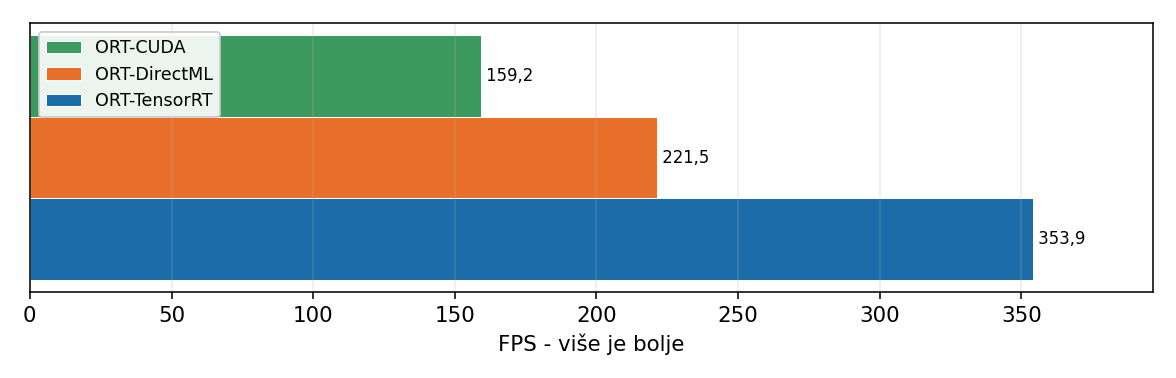
\includegraphics[width=\textwidth]{images/runtimes_ort_sr_fps.png}
	\caption{Brzina inferencije pri izvršavanju kroz ONNX Runtime sa različitim izvršnim provajderima (480p, $\times2$, prosek po modelima).}
	\label{fig:runtimes_ort}
\end{figure}

Među provajderima najbrži je TensorRT provajder, sa prosečno $353{,}9$ FPS, što je $1{,}5$ puta više od DirectML provajdera ($221{,}5$ FPS) i $2{,}2$ puta više od CUDA provajdera ($159{,}2$ FPS). Optimizacije koje TensorRT primenjuje pri izgradnji engine-a donose, dakle, znatno ubrzanje i kada se TensorRT koristi kroz ONNX Runtime. DirectML je pri tome brži od CUDA provajdera.

Slika~\ref{fig:runtimes_trt_by_size} prikazuje poređenje brzine inferencije između korišćenja TensorRT preko ONNX izvršnog okruženja i direktnog pokretanja TensorRT engine-a.

\begin{figure}[H]
	\centering
	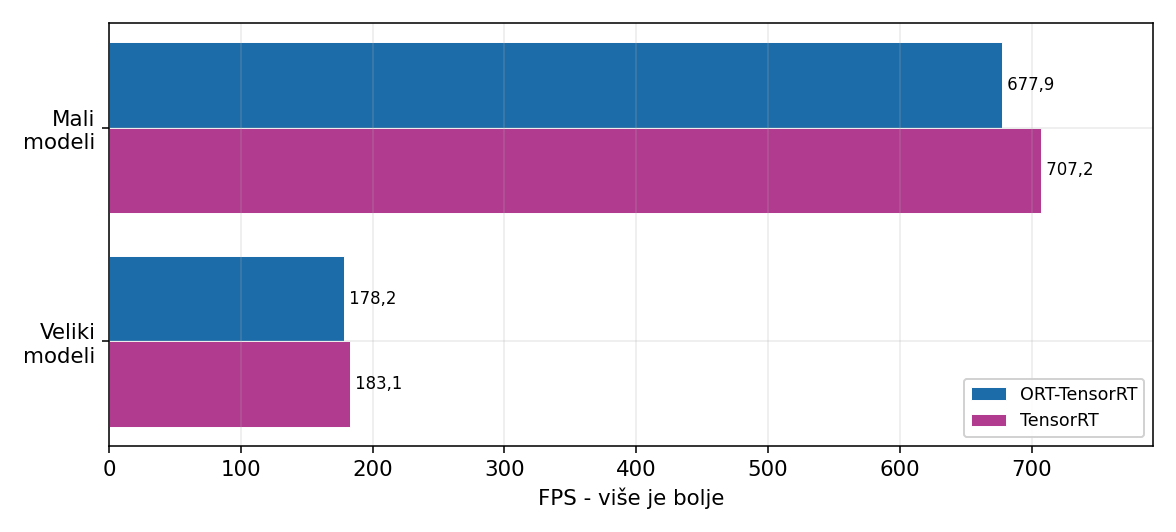
\includegraphics[width=\textwidth]{images/runtimes_ort_vs_trt_by_size_fps.png}
	\caption{Brzina inferencije pri direktnom pokretanju TensorRT engine-a i pri korišćenju TensorRT provajdera ONNX Runtime-a, za male (ispod $100$ hiljada parametara) i velike modele.}
	\label{fig:runtimes_trt_by_size}
\end{figure}

Direktnim pokretanjem TensorRT engine-a postiže se veći broj frejmova u sekundi nego kroz ONNX Runtime, ali najveća razlika je kod malih modela: $707{,}2$ naspram $677{,}9$ FPS, odnosno oko $4{,}3\%$ više. Kod velikih modela razlika je oko $2{,}7\%$. Kod malih modela samo računanje traje kratko, pa fiksni troškovi po pozivu, koje ONNX Runtime dodaje, čine veći deo ukupnog vremena.

Slika~\ref{fig:runtimes_ort_vs_trt_vs_ncnn_fps} prikazuje poređenje ONNX Runtime-a uz DirectML provajder sa izvršavanjem pomoću NCNN-a sa Vulkan ubrzanjem.

\begin{figure}[H]
	\centering
	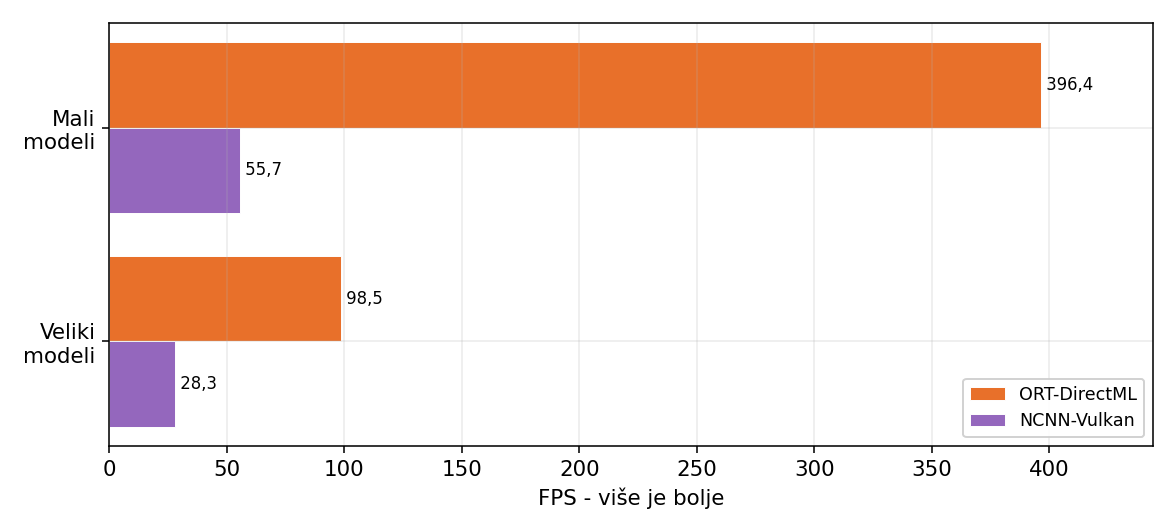
\includegraphics[width=\textwidth]{images/runtimes_ncnn_by_size_fps.png}
	\caption{Brzina inferencije pri izvršavanju pomoću NCNN-a sa Vulkan ubrzanjem i ONNX Runtime-a sa DirectML provajderom, za male i velike modele.}
	\label{fig:runtimes_ort_vs_trt_vs_ncnn_fps}
\end{figure}

NCNN je upoređen sa DirectML provajderom, jer su to jedina dva od izmerenih okruženja koja nisu vezana za grafičke kartice jednog proizvođača. NCNN je znatno sporiji: kod malih modela postiže $55{,}7$ naspram $396{,}4$ FPS, odnosno oko $7{,}8$ puta manje, a kod velikih $28{,}3$ naspram $98{,}5$ FPS, oko $3{,}4$ puta manje. Prednost NCNN-a zato nije brzina, već prenosivost, jer se, za razliku od DirectML-a, može koristiti i van Windows operativnog sistema.

Na NVIDIA grafičkim karticama najbrže je, dakle, direktno izvršavanje TensorRT engine-a, dok ONNX Runtime sa TensorRT provajderom zaostaje primetno samo kod malih modela. Za grafičke kartice drugih proizvođača pod Windows-om na raspolaganju je DirectML, koji je na korišćenoj kartici bio nekoliko puta brži od NCNN-a, a NCNN sa Vulkanom omogućava izvršavanje i na ostalim operativnim sistemima, uz manju brzinu.


\section{Implementacija demonstracionog video-plejera}
\label{sec:plejer}

Reprodukcija video-zapisa odvija se u nekoliko koraka, prikazanih na slici~\ref{fig:koraci_reprodukcije_videa}. Plejer najpre učitava fajl, a zatim ga demultipleksira, odnosno razdvaja na video i audio tok. Svaki tok je kompresovan sopstvenim kodekom, na primer H.264 za sliku i MP3 za zvuk, pa se dekodira nezavisno od drugog. Tako se dobijaju nekompresovani frejmovi i zvučni uzorci. Na kraju plejer na osnovu vremenskih oznaka usklađuje sliku i zvuk: frejmovi se prikazuju na ekranu, a zvuk se reprodukuje preko zvučne kartice.

\begin{figure}[H]
	\centering
	\resizebox{0.9\textwidth}{!}{\begin{tikzpicture}[
	node distance=4mm,
	box/.style={draw, rounded corners=2pt, align=center, font=\footnotesize,
		minimum height=10mm, text width=20mm, inner sep=1mm},
	>=stealth
	]
	% --- zajednički deo ---
	\node[box, text width=19mm] (load) {Učitavanje\\fajla};
	\node[box, text width=19mm, right=of load] (demux) {Demulti-\\pleksiranje};

	% --- video (gore) i zvuk (dole) ---
	\node[box, anchor=west] (vdec) at ($(demux.east)+(7mm,8mm)$) {Dekodiranje\\videa};
	\node[box, anchor=west] (adec) at ($(demux.east)+(7mm,-8mm)$) {Dekodiranje\\zvuka};

	% --- sinhronizacija obuhvata oba reda ---
	\node[box, text width=25mm, minimum height=26mm, anchor=west] (sync) at ($(vdec.east |- demux)+(4mm,0)$) {Sinhronizacija\\slike i zvuka};
	\node[box, text width=22mm, anchor=west] (disp) at ($(sync.east |- vdec)+(4mm,0)$) {Prikaz na\\ekranu};
	\node[box, text width=22mm, anchor=west] (play) at ($(sync.east |- adec)+(4mm,0)$) {Reprodukcija\\zvuka};

	\draw[->] (load) -- (demux);
	\coordinate (split) at ($(demux.east)+(3.5mm,0)$);
	\draw (demux.east) -- (split);
	\draw[->] (split) |- (vdec.west);
	\draw[->] (split) |- (adec.west);
	\draw[->] (vdec) -- (vdec -| sync.west);
	\draw[->] (adec) -- (adec -| sync.west);
	\draw[->] (sync.east |- disp) -- (disp);
	\draw[->] (sync.east |- play) -- (play);
\end{tikzpicture}
}
	\caption{Koraci reprodukcije video-zapisa na računaru.}
	\label{fig:koraci_reprodukcije_videa}
\end{figure}

\subsection{Mesto superrezolucije u procesu reprodukcije}

Superrezolucija se u ovaj proces uključuje kao dodatni korak u video grani, između dekodiranja i prikaza. Model obrađuje vrednosti piksela, pa se ne može primeniti na kompresovani tok, već tek na dekodirani frejm. Sa druge strane, obrada mora biti završena pre prikaza, jer se na ekranu prikazuje uvećani frejm. Mesto ovog koraka u procesu reprodukcije prikazano je na slici~\ref{fig:koraci_reprodukcije_videa_sr}.

\begin{figure}[H]
	\centering
	\resizebox{\textwidth}{!}{\begin{tikzpicture}[
	node distance=5mm,
	box/.style={draw, rounded corners=2pt, align=center, font=\footnotesize,
		minimum height=10mm, text width=20mm, inner sep=1mm},
	>=stealth
	]
	% --- zajednički deo ---
	\node[box] (load) {Učitavanje\\fajla};
	\node[box, right=of load] (demux) {Demultiplek-\\siranje};

	% --- video (gore) i zvuk (dole) ---
	\node[box, anchor=west] (vdec) at ($(demux.east)+(9mm,8mm)$) {Dekodiranje\\videa};
	\node[box, anchor=west] (adec) at ($(demux.east)+(9mm,-8mm)$) {Dekodiranje\\zvuka};
	\node[box, very thick, fill=gray!15, right=of vdec] (sr) {Super-\\rezolucija};

	% --- sinhronizacija obuhvata oba reda ---
	\node[box, text width=25mm, minimum height=26mm, anchor=west] (sync) at ($(sr.east |- demux)+(5mm,0)$) {Sinhronizacija\\slike i zvuka};
	\node[box, text width=22mm, anchor=west] (disp) at ($(sync.east |- vdec)+(5mm,0)$) {Prikaz na\\ekranu};
	\node[box, text width=22mm, anchor=west] (play) at ($(sync.east |- adec)+(5mm,0)$) {Reprodukcija\\zvuka};

	\draw[->] (load) -- (demux);
	\coordinate (split) at ($(demux.east)+(4.5mm,0)$);
	\draw (demux.east) -- (split);
	\draw[->] (split) |- (vdec.west);
	\draw[->] (split) |- (adec.west);
	\draw[->] (vdec) -- (sr);
	\draw[->] (sr) -- (sr -| sync.west);
	\draw[->] (adec) -- (adec -| sync.west);
	\draw[->] (sync.east |- disp) -- (disp);
	\draw[->] (sync.east |- play) -- (play);
\end{tikzpicture}
}
	\caption{Koraci reprodukcije video-zapisa sa dodatim korakom superrezolucije.}
	\label{fig:koraci_reprodukcije_videa_sr}
\end{figure}

I uobičajeni plejeri uvećavaju frejm kada je rezolucija prozora ili ekrana veća od rezolucije video-zapisa. To se najčešće radi bilinearnom ili bikubnom interpolacijom na grafičkoj kartici, neposredno pre prikaza. U implementiranom plejeru uvećanje preuzima model. Pošto model uvećava celobrojnim faktorom, a odnos rezolucije ekrana i video-zapisa uglavnom nije ceo broj, plejer bira najmanji podržani faktor koji nije manji od potrebnog, a interpolacija zatim samo smanjuje izlaz modela na tačne dimenzije ekrana. Na primer, za video $854\times480$ na ekranu $1920\times1080$ potrebno je uvećanje od oko $2{,}25$ puta, pa se bira faktor $3$. Veći faktor se bira namerno, jer se pri smanjivanju rekonstruisani detalji zadržavaju, dok bi uz faktor $2$ deo uvećanja ponovo obavila interpolacija. Pošto potreban faktor zavisi od rezolucije video-zapisa i ekrana, za plejer su posebno pogodni višeskalni modeli (poglavlje~\ref{sec:viseskalni}).

Uvođenje ovog koraka utiče na sinhronizaciju. Plejer prikazuje svaki frejm u trenutku određenom njegovom vremenskom oznakom, pa superrezolucija mora da se završi u okviru datog intervala $T_f$ između dva frejma (poglavlje~\ref{sec:brzina}). Frejm koji nije obrađen na vreme plejer mora da preskoči ili prikaže sa zakašnjenjem, što se primećuje kao trzanje slike. Zbog toga se za plejer bira konfiguracija modela čije vreme obrade ostavlja rezervu u odnosu na $T_f$. Pri tome se sa intervalom $T_f$ ne poredi samo vreme inferencije, već ukupno vreme obrade frejma. Dekodiranje, prenos podataka između procesora i grafičke kartice, završno skaliranje i prikaz takođe se odvijaju u okviru istog intervala. Kod malih modela ovi prateći koraci mogu trajati duže od same inferencije, pa se implementirane varijante plejera razlikuju po tome gde se ti koraci izvršavaju i koliko podataka pri tome prelazi između centralnog procesora i grafičke kartice. Implementirane su dve varijante: osnovna, u kojoj se dekodiranje, završno skaliranje i prikaz obavljaju na centralnom procesoru (odeljak~\ref{sec:osnovna_varijanta}), i zero-copy varijanta, u kojoj se svi koraci obavljaju na grafičkoj kartici, pa frejm ne napušta njenu memoriju (odeljak~\ref{sec:zero_copy}). Osnovna varijanta radi sa sva tri izvršna okruženja, dok zero-copy varijanta koristi TensorRT i hardverski dekoder NVDEC, pa zahteva NVIDIA grafičku karticu.

\subsection{Osnovna varijanta: dekodiranje i prikaz na CPU-u}
\label{sec:osnovna_varijanta}

Osnovna varijanta plejera sastoji se iz četiri dela: niti za učitavanje i dekodiranje frejmova, komponente za reprodukciju zvuka, glavne petlje koja izvršava superrezoluciju i prikaz, i izvršnog okruženja za inferenciju. Za dekodiranje i prikaz koristi se biblioteka OpenCV \cite{OpenCV}. Ovde se koristi softversko dekodiranje frejmova, odnosno dekodiranje na centralnom procesoru (CPU). Frejm koji dekodira centralni procesor zato se mora preneti na grafičku karticu (GPU), na kojoj se izvršava superrezolucija. Uvećani frejm se zatim mora vratiti u sistemsku memoriju, kako bi se na centralnom procesoru skalirao na ciljne dimenzije i prikazao pomoću funkcije \texttt{cv2.imshow}. Tok obrade jednog frejma prikazan je na slici~\ref{fig:plejer_tok}.

\begin{figure}[H]
	\centering
	\begin{tikzpicture}[
	node distance=4mm,
	box/.style={draw, rounded corners=2pt, align=center, font=\footnotesize,
		minimum height=10mm, minimum width=13mm, inner sep=1mm},
	>=stealth
	]
	\node[box] (dec) {Dekoder\\(CPU)};
	\node[box, right=of dec] (h2d) {Prenos\\na GPU};
	\node[box, right=of h2d] (pre) {Pred-\\obrada};
	\node[box, right=of pre] (sr) {SR\\mreža};
	\node[box, right=of sr] (post) {Post-\\obrada};
	\node[draw, dashed, rounded corners=4pt, inner sep=2mm, fit=(pre)(sr)(post),
	label={[font=\footnotesize]above:Izvršno okruženje (GPU)}] {};
	\node[box, right=of post] (d2h) {Prenos\\na CPU};
	\node[box, right=of d2h] (resize) {Bikubno\\skaliranje};
	\node[box, right=of resize] (disp) {Prikaz\\(OpenCV)};
	\draw[->] (dec) -- (h2d);
	\draw[->] (h2d) -- (pre);
	\draw[->] (pre) -- (sr);
	\draw[->] (sr) -- (post);
	\draw[->] (post) -- (d2h);
	\draw[->] (d2h) -- (resize);
	\draw[->] (resize) -- (disp);
\end{tikzpicture}

	\caption{Tok obrade jednog frejma u video grani osnovne varijante plejera.}
	\label{fig:plejer_tok}
\end{figure}

\subsubsection{Učitavanje frejmova}

Nit za učitavanje od dekodera traži frejmove po rednom broju, tempom koji odgovara izvornoj brzini video-zapisa. Posle svakog frejma nit na osnovu sistemskog tajmera čeka do trenutka predviđenog za sledeći. Ako dekodiranje zaostane, nit ne pokušava da nadoknadi propušteno vreme, već nastavlja od trenutnog. U osnovnoj varijanti frejmove dekodira \texttt{cv2.VideoCapture}, koji ih vraća kao NumPy niz oblika $(H,W,3)$ tipa \texttt{uint8}, u BGR rasporedu kanala. Frejmovi se dekodiraju redom, a pri premotavanju se pozicija najpre postavlja na traženi frejm:

\begin{minted}{python}
cap = cv2.VideoCapture(video_path)
fps = cap.get(cv2.CAP_PROP_FPS)

def frame(self, index):
    if index != self._next_index:
        self.cap.set(cv2.CAP_PROP_POS_FRAMES, index)
    ok, frame = self.cap.read()
    ...
\end{minted}

Nit u svakom trenutku čuva samo poslednji dekodirani frejm, zajedno sa brojačem dekodiranih frejmova. Glavna petlja proverava da li se pojavio novi frejm. Ako jeste, prosleđuje ga izvršnom okruženju, a ako nije, zadržava prethodni rezultat. Ako obrada traje duže od intervala $T_f$, nit u međuvremenu prepisuje frejmove koji nisu stigli na obradu, pa se oni preskaču. Na taj način prikaz ne zaostaje za izvornim vremenom video-zapisa, već se smanjuje broj prikazanih frejmova u sekundi ukoliko je model spor.

\subsubsection{Reprodukcija zvuka}

OpenCV ne podržava rad sa zvukom, pa se audio tok pri pokretanju plejera u celosti dekodira pomoću biblioteke PyAV \cite{PyAV} i čuva u memoriji, a reprodukuje pomoću biblioteke \texttt{sounddevice} \cite{sounddevice}. Tokom reprodukcije audio grana samo kopira uzorke. Biblioteka \texttt{sounddevice} poziva povratnu funkciju kad god zvučnoj kartici zatreba novi blok uzoraka:
\\
\\
\begin{minted}{python}
def _callback(self, outdata, frames, time_info, status):
    chunk = self.data[self._pos:self._pos + frames]
    outdata[:len(chunk)] = chunk
    self._pos += frames
\end{minted}

Zato audio grana ne utiče na superrezoluciju, a ista je u svim varijantama plejera. Slika i zvuk usklađuju se pri pokretanju, pauziranju i premotavanju.

\subsubsection{Glavna petlja}

Središnji deo petlje obrađuje samo nove frejmove i prikazuje rezultat:

\begin{minted}{python}
frame, frame_counter, pos = self._reader.get_latest()

if frame_counter != last_frame_counter or last_output is None:
    output = self._produce_display(frame)
    last_output = output
    last_frame_counter = frame_counter
    needs_redraw = True
    
if needs_redraw:
    cv2.imshow(self.window_name, last_output)
    needs_redraw = False
key = cv2.waitKeyEx(1)
\end{minted}

U osnovnoj varijanti metoda \texttt{\_produce\_display} poziva izvršno okruženje, a zatim rezultat bikubnom interpolacijom (\texttt{cv2.resize}) svodi na ciljne dimenzije. Dobijena slika prikazuje se funkcijom \texttt{cv2.imshow}, a sam prozor se osvežava tek u pozivu \texttt{cv2.waitKeyEx}, koji ujedno obrađuje događaje prozora i pritiske tastera. Ako se nije pojavio novi frejm niti je promenjeno stanje reprodukcije, petlja ne iscrtava sliku ponovo, već samo poziva \texttt{cv2.waitKeyEx}.

\subsubsection{Izvršna okruženja osnovne varijante}

Osnovna varijanta podržava sva tri izvršna okruženja opisana u poglavlju~\ref{sec:izvrsna_okruzenja}. Za plejer se sva tri ponašaju isto: primaju dekodirani frejm kao NumPy niz oblika $(H,W,3)$ u BGR formatu tipa \texttt{uint8} i vraćaju uvećani frejm oblika $(sH,sW,3)$ u istom formatu, pa je ostatak plejera nezavisan od izabranog okruženja.

ONNX Runtime prima i vraća NumPy nizove u sistemskoj memoriji, a prenose na grafičku karticu i nazad obavlja sam provajder.
\begin{minted}{python}
self.session = ort.InferenceSession(str(onnx_path), providers=provider)

def __call__(self, frame):
    return self.session.run(None, {"input": frame})[0]
\end{minted}

TensorRT engine radi isključivo sa adresama u memoriji grafičke kartice, pa prenose obavlja sam plejer, pomoću PyTorch tenzora. Frejm se prvo kopira u zaključanu (engl.\ \textit{pinned}) sistemsku memoriju, iz koje se asinhrono prenosi na grafičku karticu, a izlaz se na isti način vraća nazad. Zaključani baferi alociraju se pri prvom frejmu i zatim ponovo koriste.
\begin{minted}{python}
self.context = engine.create_execution_context()

def __call__(self, frame):
  x = self.pinned_in.copy_(torch.from_numpy(frame)).cuda(non_blocking=True)
  out = torch.empty(self.out_shape, dtype=torch.uint8, device="cuda")
  self.context.set_tensor_address("input", x.data_ptr())
  self.context.set_tensor_address("output", out.data_ptr())
  self.context.execute_async_v3(torch.cuda.current_stream().cuda_stream)
  self.pinned_out.copy_(out, non_blocking=True)
  torch.cuda.synchronize()
  return self.pinned_out.numpy()
\end{minted}

NCNN, kao i ONNX Runtime, prima i vraća podatke u sistemskoj memoriji, a prenose na grafičku karticu i nazad obavlja sama biblioteka.
\begin{minted}{python}
def __call__(self, frame):
    ...
    ex = self.net.create_extractor()
    ex.input("in0", mat_in)
    _, out = ex.extract("out0")
    ...
\end{minted}

\subsection{Predobrada i postobrada}
\label{sec:omotac}

Obrada svakog frejma obuhvata prilagođavanje ulaznih podataka formatu koji mreža očekuje, inferenciju i pripremu izlaza za prikaz. Frejmovi koje OpenCV dekoder vraća su u BGR formatu, sa celobrojnim vrednostima piksela u opsegu $[0, 255]$ i rasporedom dimenzija $(H, W, C)$. Modeli očekuju RGB ulaz u opsegu $[0, 1]$ i rasporedu $(N, C, H, W)$. U svrhu lake predobrade i postobrade kreirana je klasa \texttt{VideoWrapper}, koja služi kao omotač koji pre inferencije pretvara frejm u format modela, a nakon inferencije vraća rezultat u format pogodan za prikaz, tj. vrednosti se ograničavaju na $[0,1]$, skaliraju na $[0,255]$ i pretvaraju nazad u raspored i tip koji očekuje prikaz.

Isti omotač koristi se u svim varijantama plejera koje izvršavaju model preko TensorRT-a ili ONNX Runtime-a, a raspored ulaza i izlaza zadaje se objektom \texttt{VideoIO}. Ulaz je tipa \texttt{uint8}, u rasporedu \texttt{bgr} $(H,W,3)$, kako ga vraća dekoder na centralnom procesoru, ili \texttt{rgb} $(3,H,W)$, kako ga vraća NVDEC (poglavlje~\ref{sec:gpu_dekodiranje}). Izlaz može biti u istim rasporedima, za prikaz pomoću OpenCV-a, odnosno OpenGL-a (poglavlje~\ref{sec:gpu_prikaz}), ili \texttt{rgb\_f16}, FP16 tenzor $(1,3,sH,sW)$ sa vrednostima u opsegu $[0,255]$, kada izlaz modela zatim skalira grafička kartica (odeljak~\ref{sec:gpu_skaliranje}). Osnovna varijanta koristi kombinaciju \texttt{bgr}$\to$\texttt{bgr}:

\begin{minted}{python}
class VideoWrapper(torch.nn.Module):
  def __init__(self, model, io: VideoIO):
    super().__init__()
    self.model = model
    self.io = io
    
  def forward(self, x: torch.Tensor) -> torch.Tensor:
    # predobrada
    x = x.float() / 255.0      # uint8 [0,255] -> float [0,1]
    if self.io.input == "bgr":
      x = x[..., [2, 1, 0]].permute(2, 0, 1) # (H,W,3) BGR -> (3,H,W) RGB
    # superrezolucija  
    out = self.model(x.unsqueeze(0))
    out = torch.clamp(out, 0.0, 1.0) * 255.0
    # postobrada
    if self.io.output == "rgb_f16":
      return out.to(dtype=torch.float16)     # (1,3,sH,sW) RGB
    out = out.squeeze(0)          # (3,sH,sW) RGB
    if self.io.output == "bgr":
      out = out.permute(1, 2, 0)[..., [2, 1, 0]] # (sH,sW,3) BGR
    return out.to(dtype=torch.uint8)
\end{minted}

Omotač se izvozi u ONNX zajedno sa modelom, pa predobrada i postobrada postaju deo istog računskog grafa. Ovakva organizacija donosi dve prednosti. Prvo, konverzija tipa, normalizacija i permutacija kanala izvršavaju se nezavisno za svaki piksel, pa ih grafička kartica obavlja paralelno i znatno brže od centralnog procesora. Pošto su deo izvezenog grafa, TensorRT ih pri izgradnji engine-a može i spojiti sa susednim operacijama. Drugo, između procesora i grafičke kartice prenose se podaci tipa \texttt{uint8}, sa jednim bajtom po vrednosti, umesto dva bajta u FP16.

NCNN ne koristi ovaj omotač. Model se izvozi samo sa množenjem sa $255$ i ograničavanjem izlaza na kraju grafa, a ostatak predobrade i postobrade obavlja se na centralnom procesoru. Funkcija \texttt{from\_pixels} u jednom koraku menja raspored kanala iz BGR u RGB i raspored dimenzija iz $(H,W,C)$ u $(C,H,W)$, a vrednosti se zatim dele sa $255$. Izlaz se pomoću OpenCV-a pretvara u \texttt{uint8} i vraća u raspored $(sH,sW,3)$ u BGR formatu:

\begin{minted}{python}
h, w = frame.shape[:2]
mat_in = ncnn.Mat.from_pixels(frame, ncnn.Mat.PixelType.PIXEL_BGR2RGB, w, h)
mat_in.substract_mean_normalize([0, 0, 0], [1 / 255.0] * 3)
...
chw = np.asarray(out)  # (3,sH,sW) RGB, [0,255]
return cv2.merge([cv2.convertScaleAbs(chw[c]) for c in (2, 1, 0)])
\end{minted}


%---------------------------------------------------------------
\subsection{Zero-copy varijanta: dekodiranje i prikaz na GPU-u}
\label{sec:zero_copy}

U osnovnoj varijanti frejm po dva puta prelazi između centralnog procesora i grafičke kartice: dekodirani frejm prenosi se na grafičku karticu radi superrezolucije, a uvećani frejm vraća se u sistemsku memoriju, gde ga centralni procesor bikubno skalira i prikazuje pomoću funkcije \texttt{cv2.imshow}. Pored prenosa, centralni procesor obavlja i dekodiranje, završno skaliranje i kopiranje slike u prozor. Svi ovi troškovi mogu se izbeći ako se na grafičku karticu premeste i prvi i poslednji korak video grane. Dekodiranje tada obavlja namenski hardverski dekoder grafičke kartice, prikaz obavlja grafički API poput OpenGL-a ili Vulkana, direktno iz memorije grafičke kartice, a na grafičkoj kartici se između njih obavlja i završno bikubno skaliranje. Cela video grana ostaje na grafičkoj kartici, kako prikazuje slika~\ref{fig:plejer_tok_gpu}: centralni procesor samo upravlja tokom reprodukcije i reprodukuje zvuk, a podaci o pikselima nijednom ne prolaze kroz sistemsku memoriju (engl.\ \textit{zero-copy}).

\begin{figure}[H]
	\centering
	\begin{tikzpicture}[
	node distance=3mm,
	box/.style={draw, rounded corners=2pt, align=center, font=\footnotesize,
		minimum height=10mm, text width=16mm, inner sep=1mm},
	>=stealth
	]
	\node[box] (dec) {Dekoder\\(NVDEC)};
	\node[box, right=of dec] (pre) {Pred-\\obrada};
	\node[box, right=of pre] (sr) {SR\\mreža};
	\node[box, right=of sr] (post) {Post-\\obrada};
	\node[box, text width=19mm, right=of post] (resize) {Bikubno\\skaliranje};
	\node[box, right=of resize] (disp) {Prikaz\\(OpenGL)};
	\node[draw, dashed, rounded corners=4pt, inner sep=2mm, fit=(dec)(disp),
	label={[font=\footnotesize]above:Grafička kartica}] {};
	\draw[->] (dec) -- (pre);
	\draw[->] (pre) -- (sr);
	\draw[->] (sr) -- (post);
	\draw[->] (post) -- (resize);
	\draw[->] (resize) -- (disp);
\end{tikzpicture}

	\caption{Tok obrade frejma u zero-copy varijanti, u kojoj se dekodiranje i prikaz obavljaju na grafičkoj kartici.}
	\label{fig:plejer_tok_gpu}
\end{figure}

U nastavku se redom opisuju hardversko dekodiranje, izvršavanje modela, završno skaliranje i prikaz pomoću OpenGL-a.

\subsubsection{Hardversko dekodiranje}
\label{sec:gpu_dekodiranje}

U osnovnoj varijanti frejm dekodira centralni procesor, nakon čega se prenosi na grafičku karticu. Međutim, većina savremenih grafičkih kartica, pored jezgara namenjenih opštim izračunavanjima, sadrži i namenske hardverske blokove za dekodiranje videa. Ovi blokovi podržavaju najrasprostranjenije video kodeke, poput H.264 i HEVC, a na novijim generacijama i AV1. Kod NVIDIA grafičkih kartica ovaj blok se naziva NVDEC \cite{NVCodecSDK}, kod AMD kartica VCN, kod Intel kartica Quick Sync Video. Hardversko dekodiranje na grafičkoj kartici, nezavisno od proizvođača, donosi tri prednosti:
\begin{itemize}[itemsep=0pt]
	\item Namenski hardverski dekoder je brži od dekodiranja na centralnom procesoru i rasterećuje ga.
	\item Dekoder je zaseban hardverski blok, odvojen od računskih jedinica grafičke kartice, pa se dekodiranje velikim delom odvija paralelno sa inferencijom i ne oduzima joj računske resurse.
	\item Dekodirani frejm ostaje u memoriji grafičke kartice, pa prenos na GPU (\textit{Host to Device}) više nije potreban.
\end{itemize}

U nastavku se koristi NVDEC dekoder za NVIDIA grafičke kartice. Za pristup NVDEC-u korišćena je biblioteka PyNvVideoCodec \cite{PyNvVideoCodec}. Dekoder je podešen tako da dekodirane frejmove ostavlja u memoriji grafičke kartice i vraća ih u planarnom RGB formatu, kao tenzor oblika $(3,H,W)$ tipa \texttt{uint8}:

\begin{minted}{python}
class NvDecoder:
  def __init__(self, video_path: str, gpu_id: int = 0):
    self.decoder = nvc.SimpleDecoder(
      str(video_path), gpu_id=gpu_id,
      use_device_memory=True,            # frames stay on the GPU
      output_color_type=nvc.OutputColorType.RGBP,  # planar RGB -> (3,H,W)
    )
    md = self.decoder.get_stream_metadata()
    self.width, self.height = int(md.width), int(md.height)
    self.fps = float(md.average_fps) or 30.0
    self.num_frames = int(md.num_frames)

  def frame(self, index: int) -> torch.Tensor:
    index = max(0, min(index, self.num_frames - 1))
    return torch.from_dlpack(self.decoder[index]).clone()
\end{minted}

NVDEC sam po sebi daje frejm u formatu NV12, konverziju u RGB obavlja biblioteka, takođe na grafičkoj kartici. Dekodirani frejm predaje se PyTorch-u preko standarda DLPack \cite{DLPack}, koji omogućava da dve biblioteke dele isti memorijski blok bez kopiranja. Međutim, plejer mora da napravi kopiju frejma (\texttt{clone}) kako dekoder ne bi prepisao taj bafer novim frejmom. Ovo kopiranje se svakako izvršava unutar memorije grafičke kartice, pa je znatno jeftinije od prenosa između procesora i grafičke kartice.

\subsubsection{Izvršavanje modela}

Model se izvršava preko TensorRT engine-a izgrađenog sa omotačem \texttt{VideoWrapper} (odeljak~\ref{sec:omotac}), sa ulaznim rasporedom \texttt{rgb}. Pošto dekoder već vraća RGB frejm rasporeda $(C,H,W)$, omotač pre inferencije samo pretvara \texttt{uint8} u float, normalizuje vrednosti i dodaje dimenziju paketa. Engine se pokreće iz PyTorch-a, na zasebnom CUDA toku, a ulaz i izlaz mu se predaju kao adrese PyTorch tenzora u memoriji grafičke kartice, bez kopiranja.

\begin{minted}{python}
def __call__(self, x):
  self.stream.wait_stream(torch.cuda.current_stream())
  with torch.cuda.stream(self.stream):
    x = x.to(self.in_dtype).contiguous()
    out = torch.empty(self.out_shape, dtype=self.out_dtype, device="cuda")
    self.context.set_tensor_address(self.in_name, x.data_ptr())
    self.context.set_tensor_address(self.out_name, out.data_ptr())
    self.context.execute_async_v3(self.stream.cuda_stream)
  self.stream.synchronize()
  return out
\end{minted}

\subsubsection{Završno skaliranje i prikaz pomoću OpenGL-a}
\label{sec:gpu_skaliranje}
\label{sec:gpu_prikaz}

Nad izlazom engine-a se na grafičkoj kartici obavljaju i preostali koraci video reprodukcije, završno skaliranje i prikaz. Izlaz engine-a je RGB FP16 tenzor oblika $(1,3,sH,sW)$ sa vrednostima u opsegu $[0,255]$, koji se bikubno smanjuje na ciljne dimenzije ekrana ukoliko je to potrebno:

\begin{minted}{python}
def _downscale(self, out: torch.Tensor) -> torch.Tensor:
  if self.target_size is not None:
    out = F.interpolate(out, size=self.target_size, mode="bicubic", align_corners=False)
    out.clamp_(0.0, 255.0)
  return out.squeeze(0)
\end{minted}

Engine vraća FP16 tenzor jer bikubna interpolacija u PyTorch-u nije podržana za celobrojne tenzore. Interpolacija nije deo engine-a jer bi se tada za svaku ciljnu veličinu morao graditi poseban engine. Nakon skaliranja vrednosti se ponovo ograničavaju na opseg $[0,255]$, jer bikubno jezgro ima negativne delove, pa na oštrim ivicama može dati vrednosti izvan dozvoljenog opsega. U \texttt{uint8} se pretvara tek u okviru prepakovanja za teksturu, opisanog u nastavku.

U ovoj varijanti prikaz frejma na ekranu obavlja OpenGL \cite{OpenGL}: iscrtava se pravougaonik na kome se frejm prikazuje kao tekstura. Prozor plejera otvara biblioteka GLFW \cite{GLFW}. CUDA i OpenGL podržavaju međusobnu razmenu resursa (engl.\ \textit{CUDA--OpenGL interoperability}). To znači da se OpenGL tekstura može registrovati kod CUDA okruženja, nakon čega CUDA u nju može direktno da upisuje. Na taj način frejm od izlaza modela do ekrana ne napušta memoriju grafičke kartice i izbegava se prenos ka procesoru i nazad.

Tekstura formata RGBA8 pravi se pri prvom frejmu, u dimenzijama tog frejma, i registruje funkcijom \texttt{cudaGraphicsGLRegisterImage}. Pri registraciji se navodi da će CUDA sadržaj teksture samo upisivati i svaki put ga ceo zameniti (\texttt{cudaGraphicsRegisterFlagsWriteDiscard}), pa drajver ne mora da čuva prethodni sadržaj.

\begin{minted}[samepage]{python}
tex = GL.glGenTextures(1)
GL.glBindTexture(GL.GL_TEXTURE_2D, tex)
GL.glTexImage2D(GL.GL_TEXTURE_2D, 0, GL.GL_RGBA8, w, h, 0, GL.GL_RGBA, GL.GL_UNSIGNED_BYTE, None)
GL.glBindTexture(GL.GL_TEXTURE_2D, 0)

_, resource = rt.cudaGraphicsGLRegisterImage( int(tex), GL.GL_TEXTURE_2D, rt.cudaGraphicsRegisterFlags.cudaGraphicsRegisterFlagsWriteDiscard)
\end{minted}

Pozivi CUDA API-ja obavljaju se preko biblioteke \texttt{cuda-python} \cite{cudapython}, a pozivi OpenGL-a preko biblioteke PyOpenGL \cite{PyOpenGL}. Za svaki novi frejm izvršavaju se sledeći koraci:
\begin{enumerate}[itemsep=0pt]
	\item Model izračuna frejm uvećane rezolucije.
	\begin{minted}[samepage]{python}
			context.set_tensor_address(in_name, x.data_ptr())
			context.set_tensor_address(out_name, out.data_ptr())
			context.execute_async_v3(stream.cuda_stream)
		\end{minted}
	\item Po potrebi se rezolucija smanji bikubnom interpolacijom, tako da odgovara rezoluciji ekrana.
	\begin{minted}[samepage]{python}
			out = F.interpolate(out, size=self.target_size, mode="bicubic")
			out.clamp_(0.0, 255.0)
		\end{minted}
	\item Planarni RGB tenzor oblika $(3,H,W)$ prepakuje se u oblik $(H,W,4)$, u kome su komponente svakog piksela zapisane jedna do druge. Četvrta komponenta (alfa) dodaje se jer CUDA ne podržava registraciju tekstura sa tri komponente. Bafer za prepakovanje alocira se jednom i ponovo koristi.
	\begin{minted}[samepage]{python}
			rgba[..., :3] = frame.permute(1, 2, 0)
		\end{minted}
	\item Tekstura se mapira za CUDA pristup, čime se dobija CUDA niz (\texttt{cudaArray}) koji predstavlja njen sadržaj. Prepakovani frejm kopira se u taj niz funkcijom \texttt{cudaMemcpy2DToArray}, unutar memorije grafičke kartice. Mapiranje se zatim ukida i tekstura se vraća OpenGL-u.
	\begin{minted}[samepage]{python}
			rt.cudaGraphicsMapResources(1, resource, 0)
			_, array = rt.cudaGraphicsSubResourceGetMappedArray(resource, 0, 0)
			rt.cudaMemcpy2DToArray(array, 0, 0, rgba.data_ptr(), w * 4, w * 4, h, rt.cudaMemcpyKind.cudaMemcpyDeviceToDevice)
			rt.cudaGraphicsUnmapResources(1, resource, 0)
		\end{minted}
	\item OpenGL iscrtava pravougaonik preko oblasti iscrtavanja (\texttt{glViewport}). Šejder fragmenata za svaki piksel te oblasti uzorkuje teksturu.
	\begin{minted}[samepage]{python}
			GL.glViewport((fb_w - vw) // 2, (fb_h - vh) // 2, vw, vh)
			GL.glBindTexture(GL.GL_TEXTURE_2D, tex)
			GL.glDrawArrays(GL.GL_TRIANGLE_STRIP, 0, 4)
			glfw.swap_buffers(window)
		\end{minted}
\end{enumerate}

Engine se izvršava na zasebnom CUDA toku, nakon čega procesor čeka da engine završi obradu frejma. Preostali koraci izvršavaju se redom na podrazumevanom CUDA toku, istom koji koristi PyTorch, pa se kopiranje u teksturu izvršava tek nakon skaliranja i prepakovanja, bez dodatne sinhronizacije. Pošto je bafer za prepakovanje tipa \texttt{uint8}, pri upisu skaliranog FP16 frejma u njega istovremeno se obavlja i pretvaranje u celobrojni tip, pa za to nije potrebna zasebna operacija.

\subsubsection{Poređenje sa osnovnom varijantom}
\label{sec:doprinos_koraka}

Da bi se utvrdilo koliko pojedini delovi obrade utiču na ukupno vreme, obrada frejma deli se na tri koraka: dekodiranje frejma, superrezoluciju (\textit{sr}) zajedno sa prenosima podataka koje obavlja izvršno okruženje i prikaz, koji obuhvata završno skaliranje i prikaz slike. Merenje počinje posle $50$ frejmova zagrevanja, a vrednosti su proseci za $500$ uzastopnih frejmova. Dimenzije ciljne slike određuju se prema fiksnom referentnom ekranu rezolucije $1920\times1080$.

Slika~\ref{fig:stages} prikazuje trajanje pojedinih faza obrade frejma za model FastEDSR 4/128 na video-zapisu rezolucije 480p, u osnovnoj i u zero-copy varijanti.

\begin{figure}[H]
\centering
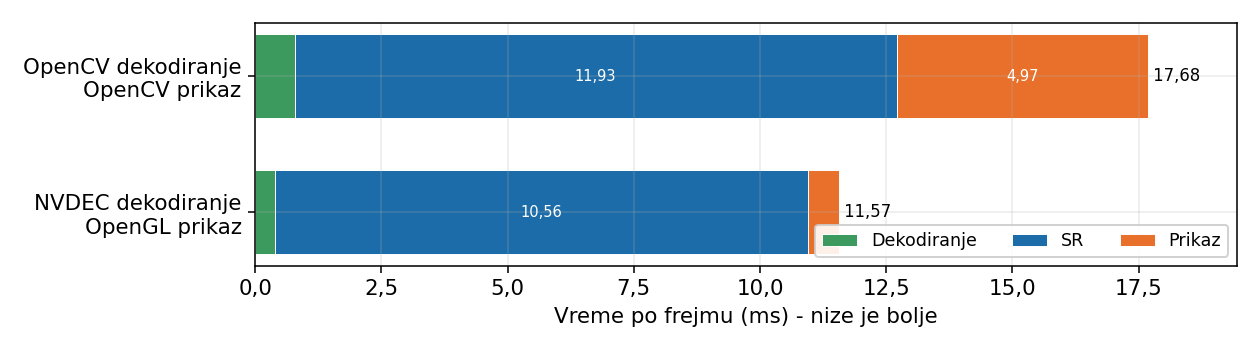
\includegraphics[width=\textwidth]{images/stages_FastEDSR_4_128.png}
\caption{Trajanje faza obrade frejma za model FastEDSR 4/128 (480p).}
\label{fig:stages}
\end{figure}

Hardversko dekodiranje skraćuje fazu dekodiranja sa $0{,}78$~ms na $0{,}48$~ms. Faza superrezolucije skraćuje se sa $11{,}93$~ms na $10{,}56$~ms, jer je dekodirani frejm već u memoriji grafičke kartice, pa izostaje njegov prenos, a izostaje i prenos rezultata nazad. Najveća razlika je u fazi prikaza: bikubno skaliranje i prikaz na centralnom procesoru traje $4{,}97$~ms, a skaliranje sa kopiranjem u teksturu samo $0{,}67$~ms. Ukupno vreme obrade frejma smanjuje se sa $17{,}68$~ms na $11{,}57$~ms. Ova razlika je izraženija kod manjih modela, kod kojih je vreme inferencije uporedivo sa vremenom dekodiranja i prenosa, dok kod većih modela inferencija čini najveći deo vremena obrade, pa je relativni dobitak manji.



%---------------------------------------------------------------
\section{Superrezolucija pomoću OpenGL šejdera}
\label{sec:gl_sejderi}

Prethodne varijante za inferenciju koriste neko izvršno okruženje za neuronske mreže i sopstveni plejer. Taj plejer je samo demonstracioni: služi za prikaz rada modela i merenje brzine, ali ne sadrži mogućnosti koje korisnici očekuju od video-plejera, kao što su podrška za titlove, plejliste ili podešavanje slike. Zato je implementiran i drugi pristup, u kome se model izvršava unutar postojećeg plejera \texttt{mpv} \cite{mpv}, video-plejera otvorenog koda (engl.\ \textit{open source}). Plejer \texttt{mpv} omogućava da se u postupak iscrtavanja frejma ubace korisnički šejderi, pa je implementiran generator koji istreniranu mrežu prevodi u niz šejdera fragmenata (engl.\ \textit{fragment shaders}), napisanih u jeziku GLSL (\textit{OpenGL Shading Language}) \cite{GLSL}. Mreža se tada izvršava na grafičkoj kartici bez ikakvog izvršnog okruženja za neuronske mreže, a za dekodiranje, skaliranje i prikaz brine sam plejer.

Šejderi (od engl.\ \textit{shading}, senčenje) su programi koji se izvršavaju na grafičkoj kartici. Pišu se u jeziku GLSL, a prevodi ih drajver grafičke kartice pri pokretanju programa. Šejder fragmenata računa vrednost jednog piksela izlazne teksture, a grafička kartica ga pokreće paralelno za svaki njen piksel. Pri tome dobija koordinate piksela koji računa i može da čita vrednosti sa proizvoljnih pozicija ulaznih tekstura, a kao rezultat vraća četiri vrednosti, koje odgovaraju komponentama RGBA. Šejder ne može da upisuje u druge piksele niti da čita rezultate koji se u istom izvršavanju računaju za druge piksele, pa se svi pikseli izlazne teksture računaju nezavisno jedni od drugih.

Na isti način radi i konvolucioni sloj, u kome se svaki izlazni piksel računa nezavisno od ostalih, iz okoline odgovarajućeg piksela ulazne mape obeležja. Osnovna ideja je zato da se svaki konvolucioni sloj mreže izvrši pomoću šejdera. Mape obeležja čuvaju se u teksturama. Šejder čita teksture prethodnog sloja i upisuje rezultat u novu teksturu, koju zatim čita sledeći sloj. Jedno takvo izvršavanje šejdera naziva se prolaz (engl.\ \textit{render pass}).

\subsection{Korisnički šejderi plejera mpv}

Korisnički šejderi učitavaju se opcijom \texttt{-{}-glsl-shaders} \cite{mpvManual}:
\begin{minted}{bash}
mpv --glsl-shaders="~~/shaders/FastEDSR.glsl" video.mp4
\end{minted}

Jedan fajl može da sadrži više šejdera. Svaki šejder počinje zaglavljem od direktiva oblika \texttt{//!NAZIV vrednost}, koje određuju kada se šejder izvršava, koje teksture čita i gde se upisuje rezultat. Iza zaglavlja sledi GLSL kod sa funkcijom \texttt{vec4 hook()}, čija se povratna vrednost upisuje u trenutni piksel izlazne teksture. Jednostavan šejder koji posvetljava sliku izgleda ovako:

\begin{minted}{glsl}
//!DESC Primer: posvetljavanje slike
//!HOOK MAIN
//!BIND MAIN
//!SAVE MAIN
vec4 hook() {
    vec4 color = MAIN_texOff(vec2(0.0, 0.0));
    return vec4(clamp(color.rgb * 1.2, 0.0, 1.0), color.a);
}
\end{minted}

Direktive imaju sledeću ulogu:
\begin{itemize}[itemsep=0pt, label=$\circ$]
	\item \texttt{//!DESC} - opis šejdera.
	\item \texttt{//!HOOK MAIN} - tačka u procesu iscrtavanja na koju se šejder „kači“. Dekodirani frejm je najčešće u formatu YUV, pa ga \texttt{mpv} najpre svodi na punu rezoluciju i pretvara u RGB. Tako dobijena slika, pre skaliranja na veličinu prozora, naziva se \texttt{MAIN}, pa šejderi dobijaju upravo sliku niske rezolucije u opsegu $[0,1]$.
	\item \texttt{//!BIND ime} - vezuje teksturu \texttt{ime} (slika \texttt{MAIN} ili tekstura koju je sačuvao neki raniji šejder) tako da šejder može da je čita.
	\item \texttt{//!SAVE ime} - rezultat šejdera se čuva u novu teksturu sa datim imenom, koju mogu da vežu kasniji šejderi. Bez ove direktive rezultat zamenjuje sliku na koju je šejder zakačen, kao u primeru iznad.
	\item \texttt{//!WIDTH} i \texttt{//!HEIGHT} - dimenzije izlazne teksture, zadate izrazom u postfiksnoj notaciji nad dimenzijama drugih tekstura. Bez njih izlazna tekstura ima dimenzije slike na koju je šejder zakačen.
	\item \texttt{//!COMPONENTS} - broj komponenti izlazne teksture, najviše četiri (RGBA).
	\item \texttt{//!WHEN} - uslov, takođe zadat izrazom u postfiksnoj notaciji, da li se šejder pokreće.
\end{itemize}

Za svaku teksturu \texttt{ime} koju šejder vezuje direktivom \texttt{//!BIND}, \texttt{mpv} automatski definiše pomoćne funkcije i promenljive: \texttt{ime\_tex(pos)} čita teksturu na normalizovanoj koordinati \texttt{pos} $\in[0,1]^2$, \texttt{ime\_texOff(off)} čita piksel pomeren za \texttt{off} piksela u odnosu na trenutni, \texttt{ime\_pos} je normalizovana koordinata trenutnog piksela u toj teksturi, a \texttt{ime\_size} dimenzije teksture u pikselima. Alokaciju tekstura i okvirnih bafera, prevođenje šejdera i njihovo izvršavanje takođe obavlja \texttt{mpv}.

Implementiran je generator šejdera za arhitekturu FastEDSR, čija je struktura dovoljno jednostavna da se svaki sloj direktno preslika u šejdere. Generator učitava težine iz sačuvanog modela, prolazi redom kroz slojeve i sve šejdere upisuje u jedan fajl sa ekstenzijom \texttt{.glsl}.

\subsection{Prevođenje konvolucija u šejdere}
\label{sec:gl_konvolucije}

Glavna ideja je čuvati mape obeležja u teksturama. Tekstura u formatu RGBA čuva četiri vrednosti po pikselu, pa jedna tekstura može da sadrži četiri mape obeležja. Izlaz sloja sa $C$ kanala se zato predstavlja sa $G = \lceil C/4 \rceil$ tekstura, koje ćemo nazivati grupama. Ove grupe ne treba mešati sa grupama kod grupisane konvolucije (engl.\ \textit{grouped convolution}), kod koje se kanali dele u grupe koje se obrađuju međusobno nezavisno. Ovde je podela na grupe samo način smeštanja kanala u teksture, a svaki izlazni kanal i dalje zavisi od svih ulaznih kanala. Ako $C$ nije deljivo sa 4, preostale komponente poslednje grupe popunjavaju se nulama.

Šejder fragmenata se izvršava nezavisno za svaki piksel izlazne teksture i računa vrednost samo tog piksela, pri čemu može da čita proizvoljne piksele ulaznih tekstura. Zato konvoluciju posmatramo iz ugla jednog izlaznog piksela $(i,j)$. Za konvoluciju $3\times3$ potrebno je izračunati težinsku sumu njegove $3\times3$ okoline preko svih ulaznih kanala, pa je vrednost izlaznog piksela:
\begin{equation}
	Y_{o,i,j} = b_o + \sum_{c=0}^{C_\text{in}-1}\ \sum_{i_k=-1}^{1}\ \sum_{j_k=-1}^{1} w_{o,c,i_k+1,j_k+1}\; X_{c,\,i+i_k,\,j+j_k},
	\label{eq:conv}
\end{equation}
gde su
\begin{itemize}[itemsep=0pt, label=$\circ$]
	\item $o \in \{0,\dots,C_\text{out}-1\}$ i $c \in \{0,\dots,C_\text{in}-1\}$ - indeksi izlaznog i ulaznog kanala
	\item $i_k, j_k \in \{-1,0,1\}$ - pomaci unutar $3\times3$ okoline piksela $(i,j)$.
	\item $Y_{o,i,j}$ - vrednost $o$-te izlazne mape obeležja na poziciji $(i,j)$
	\item $X_{c,i,j}$ - vrednost $c$-te ulazne mape obeležja na poziciji $(i,j)$, pri čemu je $X_{c,i,j} = 0$ za pozicije van slike (dopunjavanje nulama)
	\item $w_{o,c,i_k+1,j_k+1}$ - težina jezgra koje povezuje ulazni kanal $c$ sa izlaznim kanalom $o$, za pomak $(i_k,j_k)$ u odnosu na centar jezgra
	\item $b_o$ - pomeraj (engl.~\emph{bias}) izlaznog kanala $o$
\end{itemize}

Ako sve kanale jednog piksela posmatramo kao vektor, jednačina~\eqref{eq:conv} postaje
\begin{equation}
	\mathbf{y}_{i,j} = \mathbf{b} + \sum_{i_k=-1}^{1}\ \sum_{j_k=-1}^{1} \mathbf{W}_{i_k,j_k}\,\mathbf{x}_{i+i_k,\,j+j_k},
	\label{eq:conv-vec}
\end{equation}
gde su:
\begin{itemize}[itemsep=0pt, label=$\circ$]
	\item $\mathbf{y}_{i,j} \in \mathbb{R}^{C_\text{out}}$ vektor izlaznih kanala na poziciji $(i,j)$
	\item $\mathbf{x}_{i,j} \in \mathbb{R}^{C_\text{in}}$ vektor ulaznih kanala na poziciji $(i,j)$
	\item $\mathbf{b} \in \mathbb{R}^{C_\text{out}}$ vektor pomeraja
	\item $\mathbf{W}_{i_k,j_k} \in \mathbb{R}^{C_\text{out} \times C_\text{in}}$ matrica težina za jednu poziciju kernela, sa elementima $(\mathbf{W}_{i_k,j_k})_{o,c} = w_{o,c,i_k+1,j_k+1}$
\end{itemize}
 Konvolucija u jednom pikselu je, dakle, zbir devet proizvoda matrice i vektora.

Pošto šejder za svaki piksel upisuje samo jednu RGBA vrednost, jedan šejder računa samo jednu izlaznu grupu od 4 kanala, pa za izlaznu grupu $q$ važi
\begin{equation}
	\mathbf{y}^{(q)}_{i,j} = \mathbf{b}^{(q)} + \sum_{g=0}^{G_\text{in}-1}\ \sum_{i_k=-1}^{1}\ \sum_{j_k=-1}^{1} \mathbf{W}^{(q,g)}_{i_k,j_k}\,\mathbf{x}^{(g)}_{i+i_k,\,j+j_k},
	\label{eq:conv-group}
\end{equation}
gde su $\mathbf{y}^{(q)}_{i,j}, \mathbf{b}^{(q)} \in \mathbb{R}^4$ izlazni kanali, odnosno pomeraji sa indeksima $4q,4q+1,4q+2,4q+3$, a $\mathbf{W}^{(q,g)}_{i_k,j_k} \in \mathbb{R}^{4\times4}$ blok matrice $\mathbf{W}_{i_k,j_k}$ koji čine vrste $4q,4q+1,4q+2,4q+3$ i kolone $4g,4g+1,4g+2,4g+3$. 

Svaki sabirak u~\eqref{eq:conv-group} je proizvod $4\times4$ matrice i vektora dužine 4, što u jeziku GLSL odgovara jednoj operaciji \texttt{mat4 * vec4}. Sve tri sume u~\eqref{eq:conv-group} imaju unapred poznat broj članova, pa se petlje razmotavaju već pri generisanju šejdera, a težine se upisuju direktno u izvorni kod kao konstante. Za jednu ulaznu grupu ($g = 0$) dobija se:

\begin{minted}{glsl}
vec4 result = vec4(0.0);
result += mat4(0.1769, 0.1084, ...) * get_0(-1,-1);
result += mat4(...) * get_0(-1,0);
result += mat4(...) * get_0(-1,1);
result += mat4(...) * get_0(0,-1);
result += mat4(...) * get_0(0,0);
result += mat4(...) * get_0(0,1);
result += mat4(...) * get_0(1,-1);
result += mat4(...) * get_0(1,0);
result += mat4(...) * get_0(1,1);
result += vec4(-0.0151, -0.1706, -0.0361, -0.0863);
return result;
\end{minted}

Makro \texttt{get\_g(dx, dy)} čita piksel teksture grupe $g$ pomeren za \texttt{dx} kolona i \texttt{dy} vrsta u odnosu na trenutni piksel, tj.\ vraća $\mathbf{x}^{(g)}_{i+\texttt{dy},\,j+\texttt{dx}}$. Definiše se preko funkcije \texttt{\_texOff} koju obezbeđuje \texttt{mpv}, na primer \texttt{\#define get\_0(x, y) conv\_net\_0\_p0\_texOff(vec2(x, y))}. Kada sloj ima više ulaznih grupa, ovih devet redova se ponavlja za svaku od njih (\texttt{get\_1}, \texttt{get\_2}, \dots).

Za svaku izlaznu grupu generiše se poseban šejder, pa se jedan konvolucioni sloj sa $C_\text{in}$ ulaznih i $C_\text{out}$ izlaznih kanala prevodi u $G_\text{out} = \left\lceil \frac{C_\text{out}}{4} \right\rceil$ šejdera.

Teksture se imenuju po sloju mreže i grupi: izlazna grupa $q$ sloja \texttt{net.1.layers.0} čuva se u teksturi \texttt{conv\_net\_1\_layers\_0\_p}$q$. Na primer, drugi konvolucioni sloj prvog rezidualnog bloka sa $C_\text{in} = C_\text{out} = 32$ ima $G_\text{in} = 8$ ulaznih grupa, pa šejder za njegovu izlaznu grupu $q=0$ izgleda ovako:

\begin{minted}{glsl}
//!DESC net_1_layers_2 Conv3x3 part 0 chunk 0-8
//!HOOK MAIN
//!BIND conv_net_1_layers_0_p0
...
//!BIND conv_net_1_layers_0_p7
//!BIND conv_net_0_p0
//!SAVE conv_net_1_layers_2_p0
//!WIDTH conv_net_1_layers_0_p0.w
//!HEIGHT conv_net_1_layers_0_p0.h
//!COMPONENTS 4
//!WHEN OUTPUT.w MAIN.w / 1.2 > OUTPUT.h MAIN.h / 1.2 > +
#define get_0(x_off, y_off) conv_net_1_layers_0_p0_texOff(vec2(x_off, y_off))
...
#define get_7(x_off, y_off) conv_net_1_layers_0_p7_texOff(vec2(x_off, y_off))
vec4 hook() {
  vec4 result = vec4(0.0);
  result += mat4(0.0132, -0.0473, ...) * get_0(-1,-1);
  result += mat4(...) * get_0(-1,0);
  ... // 9 * 8 = 72 ovakva reda
  result += vec4(0.0021, ...);  // bias
  result += conv_net_0_p0_texOff(vec2(0.0, 0.0));   // rezidualna veza
  return result;
}
\end{minted}

Direktive \texttt{//!BIND} vezuju ulazne teksture \texttt{conv\_net\_1\_layers\_0\_p0}, \dots, \texttt{\_p7}, po jednu za svaku ulaznu grupu $\mathbf{x}^{(g)}$, i teksturu \texttt{conv\_net\_0\_p0} sa ulazom rezidualnog bloka (ovde izlaz početne konvolucije) za istu izlaznu grupu $q$, koja se na kraju dodaje rezultatu (rezidualna veza). Rezultat se direktivom \texttt{//!SAVE} čuva u teksturu \texttt{conv\_net\_1\_layers\_2\_p0}, koju vezuju šejderi narednog bloka. Sve mape obeležja imaju rezoluciju ulazne slike, pa se dimenzije izlazne teksture preuzimaju od ulazne teksture, a izlazna tekstura ima četiri komponente, jer čuva jednu grupu.

U prvom konvolucionom sloju rezidualnog bloka umesto rezidualne veze na kraju stoji aktivaciona funkcija ReLU, \texttt{result = max(result, 0.0);}. Početna konvolucija umesto tekstura sa međurezultatima vezuje samo sliku \texttt{MAIN}.

Jedan šejder može istovremeno da veže ograničen broj tekstura. Kod širih slojeva ulazne grupe se zato dele u delove od najviše $k = 8$ grupa. Svaki deo obrađuje poseban šejder, koji svoju delimičnu sumu čuva u pomoćnu teksturu (npr.\ \texttt{conv\_net\_1\_layers\_2\_p0\_c0}). Naredni deo tu teksturu vezuje, očitava je i na nju dodaje svoj doprinos.

\subsection{Završni prolaz: PixelShuffle i bilinearna osnova}
\label{sec:gl_pixelshuffle}

Završni prolaz radi u izlaznoj rezoluciji i objedinjuje operaciju PixelShuffle i sabiranje sa bilinearno uvećanim ulazom. Za piksel izlazne slike na položaju $(x,y)$ određuje se položaj unutar bloka $s\times s$, $\mathit{idx} = (x \bmod s) + s\,(y \bmod s)$, i odgovarajući piksel niske rezolucije $(\lfloor \frac{x}{s} \rfloor, \lfloor \frac{y}{s} \rfloor)$. Vrednost boje $c$ uzima se iz kanala $c\,s^2 + \mathit{idx}$ poslednje konvolucije, što je upravo preslikavanje koje obavlja PixelShuffle. Za uvećanje $\times2$ poslednja konvolucija ima $12$ kanala, odnosno tri teksture, pa je kanal $c\,s^2+\mathit{idx}$ upravo komponenta $\mathit{idx}$ teksture \texttt{p}$c$:

\begin{minted}{glsl}
//!DESC PixelShuffle x2
//!HOOK MAIN
//!BIND MAIN
//!BIND conv_upscale_block_2_0_p0
//!BIND conv_upscale_block_2_0_p1
//!BIND conv_upscale_block_2_0_p2
//!SAVE MAIN
//!WIDTH conv_upscale_block_2_0_p0.w 2 *
//!HEIGHT conv_upscale_block_2_0_p0.h 2 *
//!COMPONENTS 4
//!WHEN OUTPUT.w MAIN.w / 1.2 > OUTPUT.h MAIN.h / 1.2 > + OUTPUT.w MAIN.w / 2.2 < OUTPUT.h MAIN.h / 2.2 < + *
vec4 hook() {
  ivec2 pos = ivec2(gl_FragCoord.xy);
  ivec2 sub = pos & 1;                     // (x mod 2, y mod 2)
  int idx = sub.x + (sub.y << 1);          // polozaj u bloku 2x2

  vec2 source_pos = floor(pos / 2.0) + 0.5;   // centar LR piksela
  vec2 tex_coord = source_pos / conv_upscale_block_2_0_p0_size;

  vec4 p0 = conv_upscale_block_2_0_p0_tex(tex_coord);    // R
  vec4 p1 = conv_upscale_block_2_0_p1_tex(tex_coord);    // G
  vec4 p2 = conv_upscale_block_2_0_p2_tex(tex_coord);    // B

  vec3 res = vec3(p0[idx], p1[idx], p2[idx]);
  vec3 final_output = MAIN_tex(MAIN_pos).rgb + res; // bilinear + rezidual
  return vec4(clamp(final_output, 0.0, 1.0), 1.0);
}
\end{minted}

Promenljiva \texttt{gl\_FragCoord.xy} sadrži koordinate centra trenutnog piksela izlazne teksture. Koordinata odgovarajućeg piksela niske rezolucije deli se dimenzijama teksture (\texttt{\_size}), jer funkcija \texttt{\_tex} očekuje normalizovane koordinate. Slika \texttt{MAIN} je u ovom trenutku još uvek niske rezolucije, pa se čitanjem na koordinati \texttt{MAIN\_pos} trenutnog izlaznog piksela dobija bilinearno uvećan ulaz, koji se sabira sa rekonstruisanim rezidualom. Rezultat se ograničava na opseg $[0,1]$ i direktivom \texttt{//!SAVE MAIN} postaje nova slika \texttt{MAIN}, $s$ puta veće rezolucije. Za uvećanja $\times3$ i $\times4$ poslednja konvolucija ima $27$, odnosno $48$ kanala ($7$, odnosno $12$ tekstura), pa kanali boja više nisu poravnati sa teksturama. Završni šejder tada čita sve teksture i kanal $c\,s^2+\mathit{idx}$ bira kao komponentu $(c\,s^2+\mathit{idx}) \bmod 4$ teksture $\lfloor (c\,s^2+\mathit{idx})/4 \rfloor$.

Višeskalni model ima zajedničko telo i posebnu konvoluciju za uvećanje za svaki faktor $s\in\{2,3,4\}$. Generator zato u isti fajl upisuje šejdere tela i sve tri grane za uvećanje, a direktiva \texttt{//!WHEN} određuje koja se grana izvršava.

Posle šejdera, slika \texttt{MAIN} ima rezoluciju $s$ puta veću od frejma, ali ne nužno jednaku rezoluciji prozora. Preostalo prilagođavanje veličini prozora obavlja \texttt{mpv} svojim filtrom za skaliranje, pa se, kao i u demonstracionom plejeru, izlaz modela samo malo uvećava ili umanjuje do konačne veličine.

\subsection{Ograničenja}

Najveće ograničenje je broj prolaza, koji brzo raste sa veličinom mreže. Broj prolaza jednog sloja raste sa brojem izlaznih grupa i brojem delova na koje se dele ulazne grupe. Kada se broj kanala udvostruči, udvostručuju se obe vrednosti, pa se broj prolaza po sloju učetvorostručuje. Sloj sa $64$ ulazna i izlazna kanala zahteva $32$ prolaza, a sloj sa $128$ kanala već $128$ prolaza, pri čemu svaki novi sloj dodaje još toliko. Kod širokih i dubokih modela šejdera je zato toliko mnogo da njihovo izvršavanje u realnom vremenu praktično nije moguće.

I kod manjih modela izvršavanje pomoću šejdera je sporije nego pomoću TensorRT-a. Slika~\ref{fig:stages_shaders} prikazuje trajanje faza obrade frejma za model FastEDSR 4/32 na video-zapisu rezolucije 480p, u osnovnoj i zero-copy varijanti demonstracionog plejera i pri izvršavanju pomoću šejdera. Šejderi su za ovo merenje izvršavani u demonstracionom plejeru, uz NVDEC dekodiranje, a faza superrezolucije obuhvata i prenos ulaznog frejma u OpenGL teksturu. Superrezolucija pomoću šejdera traje $9{,}71$~ms, oko sedam puta duže nego u zero-copy varijanti ($1{,}40$~ms). Razlog je to što konvolucije u šejderima fragmenata ne koriste tenzorska jezgra, a svaki prolaz upisuje međurezultate u zasebnu teksturu u memoriji grafičke kartice i ponovo čita sve ulazne teksture. Ukupno vreme od $10{,}52$~ms je ipak dovoljno za reprodukciju u realnom vremenu, jer je i pri $60$ frejmova u sekundi na raspolaganju $16{,}7$~ms po frejmu.

\begin{figure}[H]
	\centering
	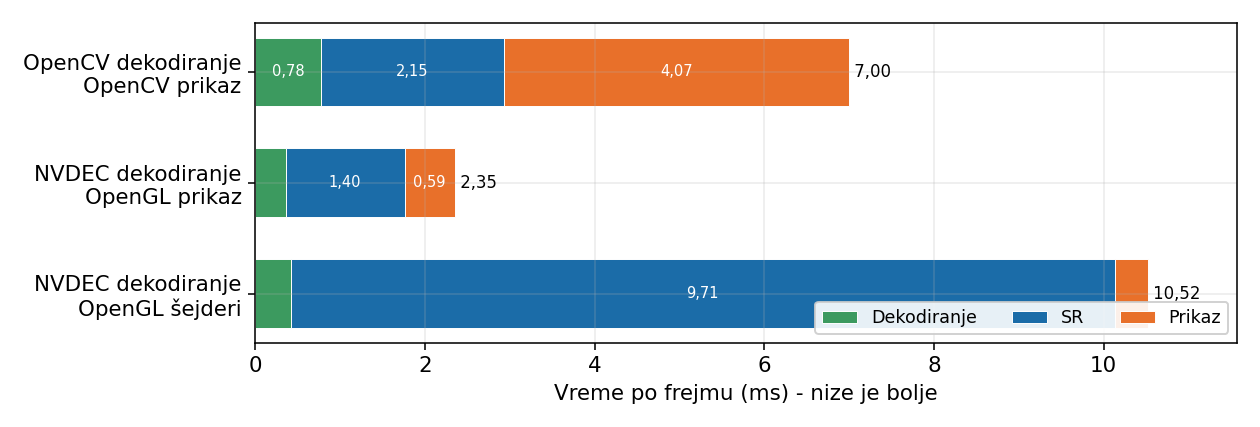
\includegraphics[width=\textwidth]{images/stages_FastEDSR_4_32_shaders.png}
	\caption{Trajanje faza obrade frejma za model FastEDSR 4/32 (480p).}
	\label{fig:stages_shaders}
\end{figure}

Prednost ovog pristupa je u tome što nije potrebno nikakvo izvršno okruženje za neuronske mreže, ni poseban plejer: dovoljan je jedan \texttt{.glsl} fajl i \texttt{mpv}, koji radi na praktično svakoj grafičkoj kartici i operativnom sistemu.

%---------------------------------------------------------------
\section{Zaključak}
\label{sec:zakljucak}

U radu je ispitana primena konvolucionih modela za superrezoluciju pojedinačne slike na uvećanje video-zapisa u realnom vremenu, gde se model primenjuje nezavisno nad svakim frejmom, pa se izbor modela ne zasniva na najboljem kvalitetu, već na kvalitetu koji se postiže unutar vremenskog budžeta jednog frejma. Šest arhitektura iz literature i predložena arhitektura FastEDSR trenirane su u velikom broju konfiguracija različite dubine i širine, a zatim primenjene u dva sistema za uvećanje video-zapisa.

Svi neuronski modeli nadmašuju klasične interpolacijske metode prema sve tri metrike. Najveće konfiguracije povećavaju PSNR za $2{,}9$ do $3{,}4$ dB u odnosu na bikubnu interpolaciju i približno dvostruko smanjuju LPIPS, dok su međusobne razlike arhitektura znatno manje od te prednosti.

Poređenje arhitektura pokazuje da efikasnost po broju parametara ne znači i efikasnost po vremenu izvršavanja. VDSR je najefikasniji po broju parametara, ali najsporiji, jer konvolucije izvršava nad $s^2$ puta više piksela. Destilacija i pažnja kod IMDN-a i RFDN-a smanjuju broj parametara, ali dodatne operacije produžavaju izvršavanje, pa ove arhitekture iznad približno $200$ FPS naglo gube kvalitet. Najbolji odnos kvaliteta i brzine imaju jednostavne mreže, ABPN i FastEDSR, koje rade u LR prostoru, sastavljene samo od konvolucija, aktivacija i sabiranja i predviđaju rezidual nad interpolacijom uvećanim ulazom.

Pokazano je i da se više faktora uvećanja može objediniti u jednom višeskalnom modelu bez gubitka kvaliteta, kao i da treniranje sa JPEG degradacijom povećava PSNR na kompresovanim ulazima u proseku za $1{,}02$ dB.

Izvršno okruženje i numerička preciznost utiču na brzinu podjednako kao i izbor arhitekture. FP16 je u proseku $2{,}13$ puta brži od FP32. Na NVIDIA grafičkim karticama najbrže je direktno izvršavanje TensorRT engine-a. TensorRT provajder ONNX Runtime-a je $1{,}5$ puta brži od DirectML-a, dok NCNN sa Vulkanom donosi prenosivost na druge operativne sisteme uz znatno manju brzinu.

Koraci van same inferencije čine značajan deo vremenskog budžeta. U osnovnoj varijanti plejera, za model FastEDSR 4/128 i video rezolucije 480p, bikubno skaliranje i prikaz na centralnom procesoru traju gotovo $5$ ms, odnosno više od četvrtine ukupnih $17{,}68$ ms. Zero-copy varijanta, sa hardverskim dekodiranjem i prikazom preko OpenGL-a, smanjuje ukupno vreme na $11{,}57$ ms, čime isti model ulazi u budžet od $16{,}7$ ms za $60$ FPS. Dobitak je relativno najveći kod malih modela, kod kojih inferencija čini manji deo ukupnog vremena.

Konačno, modeli su primenjeni u dva sistema. Prvi je demonstracioni plejer u Python-u, koji celu obradu frejma obavlja na grafičkoj kartici, a drugi generator GLSL šejdera, koji FastEDSR prevodi u šejdere za postojeći plejer \texttt{mpv}, pa se superrezolucija može koristiti bez ikakvog izvršnog okruženja za neuronske mreže i sa punim mogućnostima video-plejera.

\newpage

{\small
\let\oldthebibliography\thebibliography
\renewcommand{\thebibliography}[1]{\oldthebibliography{#1}\setlength{\itemsep}{0pt}\setlength{\parskip}{0pt}}
\bibliographystyle{ieeetr}
\bibliography{references}}


\end{document}
